%%%%%%%%%%%%%%%%%%%%%%%%%%HEADER%%%%%%%%%%%%%%%%%%%%%%%%%%%%
%%%%%%%%%%%%%%%%%%%%%%%%%%HEADER%%%%%%%%%%%%%%%%%%%%%%%%%%%%
%%%%%%%%%%%%%%%%%%%%%%%%%%HEADER%%%%%%%%%%%%%%%%%%%%%%%%%%%%
%Note: All the options like chapterprefix, pointednumbers, etc affect the way things are represented in the header of each page
\documentclass[a4paper,11pt,listof=nochaptergap,oneside,pointednumbers,bibtotoc,bigheadings,liststotoc]{scrbook}
% note that the option 'listof=nochaptergap' disables the chapter separation in listoffigures and listoftables!
% note that the expression "numbers=noenddot" remoes the dot after the number in figure captions
% for details see https://tex.stackexchange.com/questions/27250/remove-dot-after-number-in-figure-captions-while-keeping-the-dot-in-chapter-sect
\usepackage[utf8]{inputenc} %für Umlaute etc.
\usepackage[T1]{fontenc}
\usepackage[ngerman, english]{babel} %English titles (figure, table) und englische Silbentrennung
\usepackage{a4wide}
\usepackage{parskip} %see https://golatex.de/wiki/%5Cparskip to know what the package can do
\usepackage[pdftex]{color}
\usepackage{lmodern} \normalfont %to load T1lmr.fd  %weniger verpixelte Schrift; mehr Infos: http://www.namsu.de/Extra/pakete/Lmodern.html
%den genauen Trick für die untere Zeile kann ich hier nochmal nachlesen: http://tex.stackexchange.com/questions/22240/choosing-font-for-bold-small-caps-or-any-other-particular-familyseriesshape-c
\DeclareFontShape{T1}{lmr}{bx}{sc} { <-> ssub * cmr/bx/sc }{} 
\usepackage{a4} %anscheinend besser hier die Formatierung a4 wählen als als Option von documentclass
\usepackage[colorlinks = true,
		     bookmarks, 
		     linkcolor = red,
		     urlcolor = blue]{hyperref}
%\usepackage{fancyhdr}
\usepackage[right]{eurosym}
% the below two lines of code are necessary to make sure that the numbering of figures starts at 1 and then proceeds in steps of 1 instead of floating point numbers etc.
\usepackage{chngcntr}
% the below package is useful to be able to properly write down the indicator function!
\usepackage{bbm}
% lscape is to be able to put a table in landscape mode
\usepackage{lscape}
% the below is ncessary to let the footnote numbering continue over pages and chapters
\usepackage{chngcntr}
\counterwithout{footnote}{chapter}
% the below is necessary to be able to align a table by decimal points
\usepackage{dcolumn,booktabs}
\newcolumntype{d}[1]{D{.}{.}{#1}}
%\newcommand\mc[1]{\multicolumn{1}{c}{#1}} % handy shortcut macro
% the footmisc package allows multiple footnotes separated by a comma
\usepackage[multiple]{footmisc}
% the below package is necessary to be able to include in-table footnotes and make them
% show up at the bottom of the page instead of below the table
\usepackage{tablefootnote}
% package to be able to use 'bm' for boldface
\usepackage{bm}
% longtable is to be able to break a table across multiple pages
\usepackage{longtable}
\counterwithout{figure}{chapter}
\counterwithout{table}{chapter}
% the below code allows the adjustment 

\usepackage{amsmath, amssymb, amstext} %für Mathematik
\usepackage{mathstyle} %mehr Infos: http://www.ctan.org/pkg/mathstyle
\usepackage{blindtext} %to be able to place blindtext at certain locations
\usepackage[left=35mm, right=35mm, top=50mm, bottom=35mm]{geometry}%Seitenränder anpassen
\usepackage[onehalfspacing]{setspace} %1.5 Zeilgenabstand
\usepackage[round, comma]{natbib} %für die Bibliographie
%all four of the below packages are included for table creation
\usepackage{booktabs} 
\usepackage{array}
% we define new column types that take their width as argument and do
\newcolumntype{L}[1]{>{\raggedright\let\newline\\\arraybackslash\hspace{0pt}}m{#1}}
\newcolumntype{C}[1]{>{\centering\let\newline\\\arraybackslash\hspace{0pt}}m{#1}}
\newcolumntype{R}[1]{>{\raggedleft\let\newline\\\arraybackslash\hspace{0pt}}m{#1}}

\usepackage{multirow}
\usepackage{tabularx}
\usepackage{lscape}
\usepackage{mathstyle} %mehr Infos: http://www.ctan.org/pkg/mathstyle
\usepackage[pdftex]{graphicx} %to include graphics
\usepackage{microtype} % makes pdf look better
\usepackage{booktabs}
%the below package allows the modification of the enumeration symbols
\usepackage{enumerate}% http://ctan.org/pkg/enumerate
\usepackage{dcolumn} % Ausrichtung nach Dezimalpunkt in Tabellen
\newcolumntype{.}{D{.}{.}{-1}}
\usepackage{setspace}
\pagestyle{headings}
% the below code is necessary to be able to customize the font of the Figure caption for figures
\usepackage{caption} % see https://www.namsu.de/Extra/pakete/Caption.html for more information!
\captionsetup[table]{font=scriptsize,labelfont=footnotesize,labelfont=bf, singlelinecheck = false, format=hang, justification=justified, skip=10pt}
\captionsetup[figure]{font=scriptsize,labelfont=footnotesize,labelfont=bf, singlelinecheck = false, format=plain, justification=justified}%width=\dimexpr\textwidth-2cm\relax}
%\setlength{\textwidth}{15cm}
%\setlength{\textheight}{22.5cm}
%\setlength{\oddsidemargin}{1cm}
%\setlength{\evensidemargin}{0cm}
% \renewcommand{\baselinestretch}{1.2}
% \parskip1ex plus0.5ex minus0.5ex
%um die Überschriften im Inhaltsverzeichnis anzupassen
\usepackage{tocloft}
\renewcommand{\cftchapaftersnum}{.} %add period after the chapter number in ToC
% see https://tex.stackexchange.com/questions/411708/add-period-in-list-of-figures-list-of-tables
\renewcommand{\cftfigaftersnum}{.} %add period after figure number in list of figures
\renewcommand{\cfttabaftersnum}{.} %add period after table number in list of tables
\renewcommand\cftchapfont{\large\bfseries}%changes font and fontsize of chapters in toc
%\renewcommand\cftsecfont{\normalsize}
\renewcommand{\cfttoctitlefont}{\LARGE\bfseries}	%changes font of 'Content' header before toc
\renewcommand{\cftloftitlefont}{\LARGE\bfseries} %changes font of 'List of Figures'
\renewcommand{\cftlottitlefont}{\LARGE\bfseries} %changes font of 'List of Tables'
% the below commands move the beginning of toc, list of figures and list of tables further down 
% the page
\renewcommand\cftbeforetoctitleskip{2.7cm}
\renewcommand\cftbeforeloftitleskip{2.7cm}
\renewcommand\cftbeforelottitleskip{2.7cm}
%um die Überschriften im Text anzupassen
\usepackage{titlesec}
%der folgende Befehl ändert die Schriftart des "chapter"-Befehls
\titleformat{\chapter}{\large\bfseries\filright}{\LARGE\thechapter.}{15pt}{\LARGE}
\titleformat*{\section}{\large\bfseries}
\titleformat*{\subsection}{\normalsize\bfseries}
\titleformat*{\subsubsection}{\large\bfseries}
\titleformat*{\paragraph}{\small\bfseries}
% the below command is used to adjust the font-size of in-text block quotations
\usepackage{lipsum}% http://ctan.org/pkg/lipsum
\renewenvironment{quote}
               {\list{}{\rightmargin\leftmargin}%
                \item\relax\scriptsize\textquotedblleft\ignorespaces}
               {\unskip\unskip\textquotedblright\endlist}

%---------------------------------------------------------------------- Customizations ---------------------------------------------------------------------
%--------------------------------
%--------------------------------the entire below part is necessary to be able to have a 'Definition'-environment like in Math scripts.
%--------------------------------
\usepackage{amsthm}
\usepackage{amsthm}
\makeatletter
\newtheoremstyle{mysatz} %<name>
  {}% <Space above>
  {}% <Space below>
  {}% <Body font>
  {}% <Indent amount>
  {\bfseries}% <Theorem head font>
  {.}% <Punctuation after theorem head>
  {.5em}% <Space after theorem heading>
  {\thmname{#1}\thmnumber{\@ifnotempty{#1}{ }#2}%
   \thmnote{ {\the\thm@notefont(#3)}}}% <Theorem head spec (can be left empty, meaning `normal')>
\makeatother
%\theoremstyle{definition} %damit der Text innerhalb der Definition 
%nicht kursiv geschrieben wird
\makeatletter
\def\th@mysatz{%
  \thm@notefont{\bfseries}% same as heading font
}
\makeatother

\theoremstyle{mysatz}
\newtheorem{satz}{Satz}[chapter]

\newtheorem{lem}[satz]{Lemma}


\makeatletter
\newtheoremstyle{mydefinition} %<name>
  {}% <Space above>
  {}% <Space below>
  {}% <Body font>
  {}% <Indent amount>
  {\bfseries}% <Theorem head font>
  {.}% <Punctuation after theorem head>
  {.5em}% <Space after theorem heading>
  {\thmname{#1}\thmnumber{\@ifnotempty{#1}{ }#2}%
   \thmnote{ {\the\thm@notefont(#3)}}}% <Theorem head spec (can be left empty, meaning `normal')>
\makeatother
%\theoremstyle{definition} %damit der Text innerhalb der Definition 
%nicht kursiv geschrieben wird
\makeatletter
\def\th@mydefinition{%
  \thm@notefont{\bfseries}% same as heading font
}
\makeatother


\makeatletter
\newtheoremstyle{mytheorem} %<name>
  {}% <Space above>
  {}% <Space below>
  {}% <Body font>
  {}% <Indent amount>
  {\bfseries}% <Theorem head font>
  {.}% <Punctuation after theorem head>
  {.5em}% <Space after theorem heading>
  {\thmname{#1}\thmnumber{\@ifnotempty{#1}{ }#2}%
   \thmnote{ {\the\thm@notefont(#3)}}}% <Theorem head spec (can be left empty, meaning `normal')>
\makeatother
%\theoremstyle{definition} %damit der Text innerhalb der Definition 
%nicht kursiv geschrieben wird
\makeatletter
\def\th@mydefinition{%
  \thm@notefont{\bfseries}% same as heading font
}
\makeatother


\theoremstyle{mydefinition}
\newtheorem{defi}[satz]{Definition}

\theoremstyle{mytheorem}
\newtheorem{theo}[satz]{Theorem}

%\theoremstyle{remark} %damit der Text innerhalb der Bemerkung nicht
%kursiv geschrieben wird
\makeatletter
\newtheoremstyle{mybemerkung} %<name>
  {}% <Space above>
  {}% <Space below>
  {}% <Body font>
  {}% <Indent amount>
  {\itshape}% <Theorem head font>
  {.}% <Punctuation after theorem head>
  {.5em}% <Space after theorem heading>
  {\thmname{#1}\thmnumber{\@ifnotempty{#1}{ }#2}%
   \thmnote{ {\the\thm@notefont(#3)}}}% <Theorem head spec (can be left empty, meaning `normal')>
\makeatother

\theoremstyle{mybemerkung}
\newtheorem{bem}[satz]{Bemerkung}


\renewcommand{\labelitemi}{$\rhd$}



%--------------------------------
%--------------------------------the entire below part is necessary to be able to include an abstract with the books document class
%--------------------------------
\usepackage{lipsum}
\newcommand\abstractname{Abstract}  %%% here
\makeatletter
\if@titlepage
  \newenvironment{abstract}{%
      \titlepage
      \null\vfil
      \@beginparpenalty\@lowpenalty
      \begin{center}%
        \bfseries \abstractname
        \@endparpenalty\@M
      \end{center}}%
     {\par\vfil\null\endtitlepage}
\else
  \newenvironment{abstract}{%
      \if@twocolumn
        \section*{\abstractname}%
      \else
        \small
        \begin{center}%
          {\bfseries \abstractname\vspace{-.5em}\vspace{\z@}}%
        \end{center}%
        \quotation
      \fi}
      {\if@twocolumn\else\endquotation\fi}
\fi
\makeatother

%--------------------------------
%--------------------------------the entire below part is necessary to be able to customize the header
%--------------------------------

\usepackage{fancyhdr} %Paket für Kopf- und Fußzeile laden
\setlength{\headheight}{15.2pt}
\pagestyle{fancy} %wir aktivieren unseren eigenen Seitenstil
%der folgende Befehl ändert die Schriftart im Header:
\renewcommand{\chaptermark}[1]{\markboth{\chaptername\  
\thechapter. \textit{#1}}{}}
\fancyhf{} %alle Kopf- und Fußzeilenfelder bereinigen
\fancyhead[R]{\thepage}
\fancyhead[L]{\rightmark}
\renewcommand{\headrulewidth}{0.4pt} %customizing obere Trennlinie

%% a bunch of code to control the length of the headrule
%% Length to control the \fancyheadoffset and the calculation of \headline
%% simultaneously
%\newlength\FHoffset
%\setlength\FHoffset{0cm}
%
%\addtolength\headwidth{2\FHoffset}
%
%\fancyheadoffset{\FHoffset}
%
%% these lengths will control the headrule trimming to the left and right 
%\newlength\FHleft
%\newlength\FHright
%
%% here the trimmings are controlled by the user
%\setlength\FHleft{0cm}
%\setlength\FHright{0cm}
%
%% The new definition of headrule that will take into acount the trimming(s)
%\newbox\FHline
%\setbox\FHline=\hbox{\hsize=\paperwidth%
%  \hspace*{\FHleft}%
%  \rule{\dimexpr\headwidth-\FHleft-\FHright\relax}{\headrulewidth}\hspace*{\FHright}%
%}
%\renewcommand\headrule{\vskip-.7\baselineskip\copy\FHline}
%% above is a bunch of code to control the length of the headrule

% the below code creates the opportunity to include a quote at the beginning of a chapter
% customize chapter format:
\KOMAoption{headings}{twolinechapter}
\renewcommand*\chapterformat{\thechapter\autodot}

% add chapter quote to beginning of chatpers
% see https://tex.stackexchange.com/questions/53377/inspirational-quote-at-start-of-chapter
\makeatletter
\renewcommand{\@chapapp}{}% Not necessary...
\newenvironment{chapquote}[2][2em]
  {\setlength{\@tempdima}{#1}%
   \def\chapquote@author{#2}%
   \parshape 1 \@tempdima \dimexpr\textwidth-2\@tempdima\relax%
   \itshape}
  {\par\normalfont\hfill--\ \chapquote@author\hspace*{\@tempdima}\par\bigskip}
\makeatother

\newcommand\textbox[1]{%
  \parbox{.333\textwidth}{#1}%
}

%--------------------------------
%--------------------------------additional customizations
%--------------------------------
\setlength{\parindent}{0pt} %legt die Einrücktiefe der ersten Zeile für alle folgenden Absätze fest
% adds a command for exceptional paragraph identation!
\newcommand{\forceindent}{\leavevmode{\parindent=1em\indent}}
\setlength{\abovecaptionskip}{-15pt plus 3pt minus 2pt} %modify vertical space between figure and caption
\renewcommand*{\paragraph}[1]{\subsubsection*{#1} \vspace{-3mm}} %mit diesem Befehl kann man ganz einfach
%PARAGRAPH eingeben und latex macht sofort eine subsubsection ohne Nummerierung usw draus
%customizations für Vektoren (dass sie bold dargestellt werden anstatt mit einem Vektorpfeil)
\let\oldhat\hat
\renewcommand{\vec}[1]{\bm{#1}}
%\renewcommand{\hat}[1]{\oldhat{\bm{#1}}}

\newcommand{\vect}[1]{\boldsymbol{\mathbf{#1}}}
\newcommand{\hatt}[1]{\oldhat{\boldsymbol{\mathbf{#1}}}}
\newcommand{\hattnobf}[1]{\oldhat{#1}}






%%%%%%%%%%%%%%%%%%%BEGINNING OF THE DOCUMENT%%%%%%%%%%%%%%%%%%%%%%
%%%%%%%%%%%%%%%%%%%BEGINNING OF THE DOCUMENT%%%%%%%%%%%%%%%%%%%%%%
%%%%%%%%%%%%%%%%%%%BEGINNING OF THE DOCUMENT%%%%%%%%%%%%%%%%%%%%%%
\begin{document}
%----------------------------------------------------------- Beginn Titelseite -------------------------------------------------------------------------------
%\changefont{ppl}{m}{n} %mit diesem Befehl kann global ganz leicht die Schriftart geändert werden
\newgeometry{left=30mm, right=30mm, top=0mm, bottom=0mm}
\begin{titlepage}
    \begin{center}
        \hspace*{-0.27\textwidth}
\includegraphics[width=1.419\textwidth, trim = 5mm 250mm 0mm 0mm, clip = TRUE]{logo.pdf}\hspace*{-0.3\textwidth}
        \quad \\[0mm]
        \newcommand{\HRule}{\rule{\linewidth}{0.3mm}} %Befehl zum Erstellen der Linie
        \HRule \\[-1mm]
        \Huge{\scshape\bfseries Time-Varying Uncertainty and Business Cycles} \\[-5mm]
        \HRule \\[2mm]
        \Large {\scshape A Shock-Restricted Structural Vector \\
        				Autoregression Approach} \\[10mm]
        \Large Master's Thesis \\[10mm]
        \Large in partial fulfillment of the requirements \\for the degree of Master of Science (M.Sc.)\\
                  in Applied Economics \\[10mm]
                  
        submitted to\\
        Univ.-Prof. Dr. Johann Scharler \\[10mm]
        Department of Economics\\
        Faculty of Economics and Statistics\\
        Leopold-Franzens-Universität Innsbruck \\[10mm]
        by \\ Mag. Marcel A. Kropp \\[10mm]
        Innsbruck, July 2020
    \end{center}
\end{titlepage}

%----------------------------------------------------------- Ende Titelseite -------------------------------------------------------------------------------
\restoregeometry

%----------------------------------------------------------- Beginn Widmung Mum ---------------------------------------------------------------------
%Kurze Widmung an Mum.
\thispagestyle{empty} %bewirkt, dass die Striche oben wegfallen und, dass die Seitenzahl wegfällt.
\null\vspace{\stretch{1}}
    \begin{flushright}
       \large \textit{To my Mum.}\\
    \end{flushright}
\vspace{\stretch{2}}\null
%----------------------------------------------------------- Ende Widmung Mum ------------------------------------------------------------------------


%----------------------------------------------------------- Beginn Widmung Alle ------------------------------------------------------------------------
\newpage
\thispagestyle{empty} %bewirk, dass die Striche oben wegfallen und, dass die Seitenzahl wegfällt.


%\topskip0pt
\vspace*{60px}
I want to thank my supervisor, Prof. Dr. Johann Scharler (University of Innsbruck) who was incredibly supportive and patient throughout the entire writing process and subsequent finalization of this thesis which got delayed in the midst of switching between two full-time jobs.

I am indebted to Dr. Martin Geiger (Liechtenstein-Institut, University of Innsbruck) as well as Max Breitenlechner, PhD (University of Innsbruck) who have helped me kick-start my research into the world of uncertainty and business cycles in valuable and helpful sessions in their office at the University of Innsbruck. 

Having set up the shock-restricted SVAR-algorithm as proposed by \citet{ludvigsonetal:18} in R and having detected discrepancies between the author's IRFs and my own, Sai Ma, PhD (one of the co-authors of \citet{ludvigsonetal:18}; Federal Reserve Board of Governors) has kindly provided me with the Matlab-code of their Baseline-scenario which helped me to detect errors in my own implementation.\\

What I wrote when handing in the diploma thesis for my first degree still holds more than ever:

My family has been my strongest support in all my life. I especially want to express my gratitude to my dear uncle Dr. med. Farshid Mavaddat, my cousins Dr. Paik Saber and Neisan Saber and my aunt Mahshid Mavaddat.\\
Most of all I want to thank my Mum, Dorrie Mavaddat, who has always been there for me and supported and helped me in all my ventures. It is due to her that I stand where I am today.
    \begin{flushright}
         Innsbruck, July 2020\\
    \end{flushright}
\vspace*{\fill}
%
\pagestyle{headings}
%-------------------------------------------------------------- Ende Widmung Alle ------------------------------------------------------------------------

%\clearpage
%\setlength{\hoffset}{0mm}

%jetzt kommen die abstracts auf Englisch und Deutsch
\thispagestyle{empty} 
%\quad \\[2cm]
\selectlanguage{english}
\begin{abstract}
% \blindtext
Uncertainty is a latent and generally unobservable stochastic process. Insofar, the uncertainty literature which experienced a renaissance with the publication of \citet{bloom:09} is largely trying to solve both, questions related to the measurement and \textit{types} of uncertainty and, most prominently, the role of time-varying uncertainty on and in business cycles, respectively. In the meantime a voluminous amount of both theoretical and empirical work has produced various uncertainty measures that, in various empirical VAR-settings, largely suggests that uncertainty exerts a negative influence on the business cycle. Departing from usual recursive schemes in VARs which don't allow for the link between uncertainty and business cycles to contemporaneously go vice-versa by construction, \citet{ludvigsonetal:18} suggest a novel shock-restricted SVAR-approach whose technicalities we discuss and replicate/implement in R for this thesis. The results indicate that, first, the uncertainty literature has to distinguish between macroeconomic and financial uncertainty and, second, that higher macroeconomic uncertainty is an endogenous \textit{response} to shocks to aggregate output while financial uncertainty can be seen as a likely source for protracted declines in aggregate output.
\end{abstract}

%\quad \\[10mm]
\begin{otherlanguage}{ngerman}
\begin{abstract}
% \blindtext
Unsicherheit ist ein latenter und im Allgemeinen nicht beobachtbarer stochastischer Prozess. Insofern versucht die Literatur, die mit der Veröffentlichung von \citet{bloom:09} eine Art Renaissance erfuhr, weitgehend sowohl Fragen zur Messung und den \textit{Arten} von Unsicherheit als auch, vor allem, zur Rolle zeitlich variierender Unsicherheit auf bzw. in Konjunkturzyklen zu beantworten. In der Zwischenzeit hat eine umfangreiche Zahl von sowohl theoretischen als auch empirischen Arbeiten verschiedene Unsicherheitsmaße vorgeschlagen, die in verschiedenen empirischen VAR-Anwendungen weitgehend darauf hindeuten, dass Unsicherheit einen negativen Einfluss auf den Konjunkturzyklus ausübt. Abweichend von den üblichen rekursiven Ansätzen in VAR-Modellen bei denen der Zusammenhang zwischen Unsicherheit und der Konjunktur bereits per Konstruktion nicht gleichzeitig einen umgekehrten Impuls geben kann, schlagen \citet{ludvigsonetal:18} einen neuartigen Schock-beschränkten SVAR-Ansatz vor dessen technischen Details wir in dieser Arbeit darstellen und in R replizieren/implementieren. Die Ergebnisse deuten darauf hin, dass, Erstens, in der Unsicherheits-Literatur zwischen makroökonomischer und finanzieller Unsicherheit unterschieden werden muss und, Zweitens, dass eine höhere makroökonomische Unsicherheit eine endogene Reaktion auf Konjunktur-Schocks ist, während finanzielle Unsicherheit eine wahrscheinliche Quelle für langwierige Konjunktureinbrüche darstellt.
\end{abstract}
\end{otherlanguage}






\restoregeometry

\thispagestyle{empty}
\pagestyle{fancy} %bewirkt, dass die Striche oben wieder dazukommen
\pagenumbering{roman} %bewirkt, dass LateX i, ii, usw zählt
\setcounter{page}{7} %und aber schon bei 7 anfängt zu zählen
%\renewcommand{\contentsname}{Table of Contents}
%\renewcommand{\cftdot}{\ensuremath{\ast}} %\ensuremath{\ast} does sth funny to the dots in the toc
\tableofcontents
\newpage
\listoffigures

\newpage
\listoftables

\newpage

%%%%%%%%%%%%%%%%AB HIER BEGINNT DER INHALT DER ARBEIT%%%%%%%%%%%%%%%%%%%%%
%%%%%%%%%%%%%%%%AB HIER BEGINNT DER INHALT DER ARBEIT%%%%%%%%%%%%%%%%%%%%%
%%%%%%%%%%%%%%%%AB HIER BEGINNT DER INHALT DER ARBEIT%%%%%%%%%%%%%%%%%%%%%
\pagenumbering{arabic} %mit diesem Befehl wechseln wir auf 1, 2, 3, usw. zum zählen.


%%%%%%%%%%%%%%%%%%%%%%%%%%INTRODUCTION%%%%%%%%%%%%%%%%%%%%%%%%%
%%%%%%%%%%%%%%%%%%%%%%%%%%INTRODUCTION%%%%%%%%%%%%%%%%%%%%%%%%%
%%%%%%%%%%%%%%%%%%%%%%%%%%INTRODUCTION%%%%%%%%%%%%%%%%%%%%%%%%%
\chapter{Introduction}
\label{introduction}
% the below code making use of "begingroup" etc. is only necessary if I want to customize the font for a particular part of the thesis
%\begingroup
%\fontsize{10pt}{12pt}\selectfont
It can be commonly postulated that being faced with uncertainty is a state inherent to life's existence and in every aspect a natural part of our complex world.

Focussing on \textit{economic} uncertainty, \href{http://citeseerx.ist.psu.edu/viewdoc/download?doi=10.1.1.334.4248&rep=rep1&type=pdf}{an investor being concerned about the performance of her assets, an employee being worried about future income streams during retirement or at all still having a job one year from now or a business continuously defending its position on the market are just a few examples} of individuals or a collective being exposed to uncertainty in every-day life. Many of these risks/uncertainties\footnote{Note that we are currently still using these terms interchangeably but will give a brief overview of the discussion and their subtle differences in the literature below.} have given rise to institutions and entire industries as an integral part of today's modern economies: sophisticated financial markets (with their risk-transformation-function being a pivotal element besides the purpose to raise capital) and the finance and insurance industry would not exist (or albeit in a different form) if it was not for the existence of uncertainty. On the academic front, ever more complex models promise remedy to make exposures to uncertainty and foresight calculable and/or manageable.

Going beyond these exemplary scenarios where economic agents seem to take into account some sort of probabilistic assessment of the future turn of events, on an aggregate (macro) level specific (tail) events can cause (economic or political) uncertainty to ultimately feed into the micro-level (firms and households) in a potentially damaging way, being rather perceived as exogenous shocks (i.e., outside of one's own area of influence) than part of a known probabilistic state space.

\href{https://site.stanford.edu/2018/session-6}{As aptly formulated by Nicholas Bloom}\footnote{Bloom is part of a larger group of contributors to the most recent macroeconomic literature that has started to systematically disentangle the effects of uncertainty both theoretically and empirically.}, after the Great Recession, the subsequent turmoil in the Eurozone's sovereign debt markets and the Arab Spring being just a few examples, the most recent major political events\footnote{One could potentially also call them 'shocks'.} of Brexit, Trump's election in the US,  the trade war with China and a seeming worsening of the relationship between forces of the West and East have intensified concerns about uncertainty. Assessments from the 
\citet{FOMC:09}\footnote{``Widespread reports from business contacts noted that uncertainties about health-care, tax, and environmental policies were adding to businesses' reluctance to commit to higher capital spending'' \citep{FOMC:09}.} and the International Monetary Fund \citep{IMF:12, IMF:13}\footnote{``More seems to be at work, however [...] - namely, a general feeling of uncertainty'. Assessing the precise nature and effects of this uncertainty is essential, but [...] not easy. [...] Uncertainty appears more diffus, more Knightian in nature.'' \citep{IMF:12}. In \citet{IMF:13} the authors dedicated a whole section (pp. 70-67) to the study of the effects of uncertainty, stating that ``[a] common view is that high uncertainty in general, and high policy uncertainty more specifically, has held back global investment and output growth in the past two years.'' \citep[p. 70]{IMF:13}.}, for example, suggest how multilayered uncertainty can be by referring to how factors such as ``[...] U.S. and European fiscal, regulatory, and monetary policies [have] contributed to a steep economic decline in 2008-2009 and slow recoveries afterward.'' \citep[p.1594]{bakeretal:15}\\
\\
On a high level, \citet{dequesh:00} identifies four basic social practices in today's societies that have a stabilizing effect on the coexistence in our (as  he calls it) \textit{economic reality}: (1) legal contracts (that reduce the uncertainty of future values of nominal variables), (2) the 'State' which enforces legal contracts in case one party to a contract would decide to not fulfill its obligations, (3) Market-Makers (a very prominent example being central banks in their roles as lenders of last resort), and lastly, (4) informal institutions including conventions like 'socially shared and/or prescribed standards of thought and behavior'. \\
Together these features improve subjective and objective uncertainty but can obviously not completely eliminate it.\\
\\
And whoever analyses \textit{uncertainty} and its underlying meaning in the literature hoping to clearly differentiate it from related concepts such as \textit{risk} or \textit{ambiguity}, will quickly realize that an unambiguous definition is not straightforward. Confining ourselves to economics only, there is a vast array of literature starting at the beginning of the 20th century that refers to these concepts in different schools of thought that at their core do have a philosophical component to them. Different parlance within the profession which \href{http://www.economics-ejournal.org/economics/discussionpapers/2015-36/file}{even causes similar concepts to be named differently} or the same term being used with a different meaning additionally complicates matters.\\
\\
While a thorough discussion of every aspect of the related concepts is beyond the scope of this work, we still want to give a brief overview of a few insights by referring to a few selecting writings:

\citet{dow:16} tries to clarify the difference between the mainstream and Keynesian\footnote{Keynes and Knight are often-times regarded as the two prominent figures that introduced the concept of \textit{fundamental uncertainty} into the economic sciences.} understanding of \textit{uncertainty}\footnote{\citet{dow:16} also makes account to von Mises, Hayek and Shackle who have also dealt with uncertainty in their works but focusses on Keynes's views on fundamental uncertainty arguing for it to be the most developed and philosophically-grounded counterpoint to the mainstream theory.}, its distinction from \textit{risk} and the resulting theoretical implications\footnote{Note that there are also schools that reject the distinction between \textit{uncertainty} and \textit{risk} altogether (e.g., \citealp{savage:54}).}. According to her assessment, in the traditional mainstream analysis within a Bayesian framework most knowledge is viewed as known or known to be stochastic in some form (called \textit{risk}), meaning that the state space is known and numerical probabilities can be assigned. Under this approach, mainstream traditional macroeconomic models give only very limited room, if any, to \textit{uncertainty} as a state of absence of such probabilities in the form of exogenous sources of shocks\footnote{\citet[p. 43]{dequesh:00} refers to some economists partly neglecting fundamental uncertainty following the argument that it might lead to 'theoretical nihilism' (see e.g., \citealp{coddington:82}).}.

Read from this dualistic mainstream perspective, \citet{dow:16} asserts that Keynes' standpoint was also for a long time interpreted in a dualistic way, albeit flipped in the sense that only in special circumstances, knowledge (here referred to as \textit{risk}) could be treated as certain and (fundamental) uncertainty was regarded as the general case (see the introduction in \citealp{keynes:21}). This dualistic interpretation was seemingly reinforced by Keynes's reflections on long-term expectations: ``About [uncertainty] there is no scientific basis on which to form any calculable probability whatever. We simply do not know'' \citep[p. 214/214]{keynes:37}.

But \citet{dow:16} clarifies that in the meantime it is well-established that Keynes did not give up on scientific knowledge (i.e., did not advocate nihilism) by giving so much weight to uncertainty but that his view on uncertainty is rather multidimensional and consists of various degrees. As an advocate of this view, \citet{dequesh:00} argues that Keynes referred to both ambiguity in his early writings (\citealp{keynes:21})\footnote{According to interpreters, in terms of \citet{keynes:21}, for both ambiguity and fundamental uncertainty there is no basis for the assignment of point, numerical probabilities \citep{dequesh:00}.} and fundamental uncertainty in his later ones (\citealp{keynes:37}) and that simply speaking of Keynesian uncertainty may actually be too vague in most circumstances.

\citet[p. 330]{camererandweber:92} describe ambiguity as ``uncertainty about probability, created by missing information that is relevant and could be known''. \citet[p. 623]{dequech:14} states that while usually the decision-maker under ambiguity cannot reliably assess the probability of each event, she usually knows all possible events (or it is at least ``predetermined or knowable ex ante``) while the case of fundamental uncertainty ``[...] is characterized by the possibility of creativity and non-predetermined structural change''. So under this concept and ``[w]ithin the bounds imposed by natural laws, the list of possible events is not predetermined or knowable ex ante [...] as \textit{the future is yet to be created}\footnote{Italics added.}'' \citep[p. 623]{dequech:14}.\footnote{\citet{dequesh:00} sees the work of \citet{shackle:72} as advocating this argument.}

With regard to fundamental uncertainty, \citet{dequesh:00} mentions technological or managerial innovations as examples of human creativity that can disrupt our realities which is closely connected to the process of creative destruction of \citet{schumpeter:42}. Unpredictable structural changes (e.g. historical changes) to our economic reality on the other hand are more typically political, social or cultural disruptions where institutions and technological change play a key-role. Interestingly, the capitalist system as we know it is regarded as endogenously causing uncertainty due to competing economic actors and decision-makers innovating in search for extra profits (see \citealp{kregel:87})\footnote{Despite of the above remarks, Keynes' notion of uncertainty as described in \citet{keynes:21} and its connection to \citet{keynes:37} has been subject to much controversy due to differing interpretations \citep{dequesh:00}.}.

Coming back to the mainstream view, while the crisis and subsequent Great Recession has triggered a rethinking of the mainstream approach to uncertainty by emphasizing ``institutional impediments to information access (asymmetric information)'' \citep[p. 8]{dow:16}, degrees of uncertainty were only gradually added to the picture: the term 'ambiguity' was acquired as well (also following \citealp[p. 330]{camererandweber:92}) to account for these various degrees of uncertainty while 'unknown unknowns' (i.e. unimaginable events or 'black swans' as dubbed by \citealp{taleb:08}) would have to be seen as \textit{'knowable unknowns'} to still be consistent with the Bayesian framework. The term 'ambiguity' is thereby introduced as falling either into the category of risk or uncertainty depending on the ability to quantify higher-order probabilities.\\
\\
Trying to establish a typology within the introduced terms, \citet{dequech:14}  sets up three dimensions along which he classifies relevant concepts\footnote{Apart from this classification we do not discuss any further interrelationships between the various concepts.}: 
\begin{enumerate}
	\item between substantive and procedural uncertainty:\footnote{Proposed by \citet[p. 145]{dosiandegidi:91} whereby substantive uncertainty results from the ``lack of all the information which would be necessary to make decisions with certain outcomes'' and procedural uncertainty from ``limitations on the computational cognitive capabilities of the [respective] agents to pursue unambiguously their objectives, given [...] available information'' in a complex decision problem. }
	\item between weak and strong uncertainty:\footnote{Whereby under weak uncertainty ``[...] an agent can form [...] a unique, additive and fully reliable probability distribution'' based on relevant and good-quality information and strong uncertainty consequently ``[...] by the absence of such a distribution'' \citep[p. 622/623]{dequech:14}.} \\
	weak uncertainty is then further subdivided into \textit{Knightian risk} (see \citet{knight:21}; often simply called 'situations of risk' where agents are faced with objective probabilities, either a priori or statistical probabilities (i.e., relative frequencies) and \textit{Savage's uncertainty} (see \citet{savage:54}; who introduced a full theory of 'personal probability' where \textit{personal} belief governs probabilities, based on prior \href{https://archive.org/stream/in.ernet.dli.2015.223806/2015.223806.The-Foundations#page/n289/mode/2up}{groundbreaking work of} \href{http://www.brunodefinetti.it/Link/Subjective%20Expected%20Utility%20-%20Intro.htm}{\citet{ramsey:26}\footnote{Written ``in opposition'' to \citet{keynes:21}.} and \citet{finetti:37}});
	\item between ambiguity and fundamental uncertainty.\footnote{Which are two types of strong and substantive uncertainty \citep{dequesh:00}.}
\end{enumerate}
\vspace{1cm}


Abstracting from the (in parts philosophical) considerations above, the question arises as to whether there is any consent in the literature about whether uncertainty can be quantified and, if so, how this could be achieved? And once having a meaningful measure of unertainty, what \textit{real} effect, if any, does it exert on business cycles?\\

Within the past ten years and largely triggered by a seminal work by \citet{bloom:09}\footnote{Bloom's contribution triggered a wave of studies that challenged the effects that he had reported in his initial publication in \citet{bloom:09}. We will come back to his study in Section~\ref{sec:selectedworkindetail}.}, macroeconomists have started studying these questions more intensively than ever before. At a first glance, as summarized by \citet[p. 1177]{juradoetal:15}, partial equilibrium analyses to date suggest that increased levels of uncertainty ``[...] can depress hiring, investment, or consumption if agents are subject to fixed costs or partial irreversibilities (a 'real options' effect), if agents are risk averse (a 'precautionary savings' effect), or if financial constraints tighten in response to higher uncertainty (a 'financial frictions' effect).''

But as aptly formulated by \citet[p. 24]{bontempietal:16}, the results found in the literature to date are not unambiguous and, among others, raise the following \textit{key}\footnote{Italics added.} questions:\footnote{We have slightly adapted/extended \citet{bontempietal:16}'s objections.}
\begin{enumerate}
	\item Are uncertainty shocks temporary or more persistent?
	\item Is the degree of persistence of identified negative uncertainty effects related to the econometric specification and/or the particular (type of) uncertainty measure used? 
	\item Does the time span over which a model is estimated play any role? \\
	And finally:
	\item Are uncertainty shocks an exogenous impulse or an endogenous response to macroeconomic fluctuations (as posed by \citealp{ludvigsonetal:18})? In other words, is uncertainty a decisive factor contributing to business cycles or does the causation go vice versa?
\end{enumerate}

The remainder of this thesis is organized as follows. Section~\ref{UncertaintyandBusinessCyclesRelatedLiterature} reviews a selection of the related literature triggered by the seminal work of \citet{bloom:09} and thereby elaborates on potential shortcomings of the popularized econometric approaches, Section~\ref{EconometricModel} hence introduces the econometric framework of \citet{ludvigsonetal:18} that tries to alleviate the identified shortcomings by shedding light on the question of whether uncertainty shocks are an exogenous impulse (as frequently postulated in the literature) or an endogenous response to uncertainty shocks and whether the particular \textit{type} of uncertainty matters by utilizing a novel shock restricted structural vector autoregression (SVAR) approach. Section~\ref{sec:Data} gives an overview of the data used and Section~\ref{Results} presents the results of their Baseline-model which we have implemented in R. Section~\ref{Conclusion} finally summarizes and concludes. Additional information and results are deferred to Appendix~\ref{VARAndLocalProjection} and Appendix~\ref{DataAndCode}, respectively.



%%%%%%%%%%%%%%%%%%%%%LITERATURELITERATURE%%%%%%%%%%%%%%%%%%%%%%%%
%%%%%%%%%%%%%%%%%%%%%LITERATURELITERATURE%%%%%%%%%%%%%%%%%%%%%%%%
%%%%%%%%%%%%%%%%%%%%%LITERATURELITERATURE%%%%%%%%%%%%%%%%%%%%%%%%
\chapter{Related Literature}
\label{UncertaintyandBusinessCyclesRelatedLiterature}

While uncertainty in theoretical and empirical applications has been dealt with already long before the Great Recession, it is safe to say that research in the field surged in the past decade to understand the relationship between uncertainty and business cycles and to put, among others, arguments that point at increased uncertainty as a possibly compounding factor to the Great Recession and subsequent slow recovery on steadier grounds. 

This growing body of literature covers the entire spectrum including studies examining the matter from (i) a solely theoretical, (ii) purely empirical or (iii) both perspectives in both micro- and macroeconomic analyses. In our review below we will refer to works falling into either of the three categories whereby contributions having both an empirical and theoretical component are in a slight majority.  Note, however that also purely theoretical or empirical works often pick up previous theoretical or empirical results that have been reported in the literature and thereby all the more establish a theory-empirics-nexus. Further, while the Great Recession is frequently mentioned as a reference, the implications of the results are often-times generalized without specific attribution to the Great Recession. At most, key economic features (e.g. zero lower bounds, etc.) are considered in model extensions.\footnote{An exception is \citet{schaal:17} that investigates the fit of his model to the data  ...} 

Empirically, various analyses have produced seemingly unambiguous results in various identification schemes predominantly in a VAR-framework thereby deploying different uncertainty proxies in an attempt to measure the underlying latent stochastic process (since uncertainty is an intrinsically unobservable concept as formulated by \citep{bloom:14}. But as we will discuss in the following, these empirical findings result from the econometric specifications which might be problematic. Theoretically, most models stress contractionary effects of uncertainty although diametrical effects might be at work as well. Abstracting from problems revolving around the \textit{measurement} of uncertainty and empirical analyses and deferring them to Sections~\ref{sec:uncertaintymeasuresandstylizedfacts} and \ref{sec:selectedworkindetail} first, Section~\ref{sec:studiedeffectsinrelatedliterature} below starts with an overview of the theoretical behavioural channels that have been identified in the literature, Section~\ref{sec:selectedworkindetail} subsequently presents a few contributions in greater detail including an analysis of their econometric frameworks in VAR-settings.\footnote{Besides theoretical approaches, one part of the empirical literature uses micro-data (mostly firm-level data) in an attempt to extract uncertainty effects.} Section~\ref{sec:robustnessofeconspecs} looks at the robustness of the VAR-results while Section~\ref{sec:uncertaintymeasuresandstylizedfacts} takes a brief look at the ambiguous definition of uncertainty in the literature and stylized facts of a few selected and popular uncertainty measures. Section~\ref{sec:exoEndoJuradoetal} finally concludes the discussion and presents the main research question which is whether uncertainty can be seen as the source of economic fluctuations or itself endogenously responds to business cycles.


\section[Theoretical Behavioural Channels, \textit{or}: The Micro-Macro-Nexus]{Theoretical Behavioural Channels, \textit{or}: The Micro-Macro-Nexus}
\label{sec:studiedeffectsinrelatedliterature}

In the microeconomics literature, there is no single uncertainty theory and various mechanisms have been identified through which aggregate uncertainty suggests to play a role in altering economic agent's behavior which in turn adversely (and in some cases positively) affects economic activity. In particular, the literature largely evolves around \textit{real-options-} (on which a large part of the literature has focussed so far), \textit{risk-aversion-},\footnote{\textit{Precautionary savings} effects are classified somewhere in-between. See below for details.} \textit{risk premia-} and \textit{Oi-Hartman-Abel effects} that help forming a better understanding of the forces at work.\footnote{This taxonomy is based on \citet{bloom:14}.} While the mentioned effects are partial equilibrium effects (PE; ceteris paribus effects) with generally unambiguous signs in isolation, together in one combination or another in general equilibrium (GE) analyses the net effects on investment, consumption unemployment and the access to finance might be less explicit due to equilibrating price and quantity changes.\\

The \textit{real-options-effect} primarily applies to firms (investment and hiring decisions) but has also been expanded to households (consumption and thus savings decisions). 

In the case of firms the real-options effect gave rise to the analysis of business cycle dynamics within the traditional framework of irreversible investment: when being faced with uncertainty firms become more cautious about investment and hiring if those decisions cannot easily be reversed (so-called 'investment adjustment costs') which is summarized under the \textit{delay effect}.\footnote{These option-effects are alleviated, however, if, on the other hand, delays would be so costly as to hamper firm's ability to wait.} More specifically, a company acquiring capital for a purchase price that will differ from the resale price essentially buys a put option and through an investment today forgoes a call option (i.e., the chance to buy later). In an environment of higher uncertainty the value of a call option increases (an incentive to postpone investment to avoid costly mistakes) while with respect to partial reversibility the value of a put option that is being obtained by investing today increases with uncertainty, leaving the overall effect ambiguous. These (partial) irreversibilities have been introduced as an answer to the \textit{Oi-Hartman-Abeld}-effect (which we introduce below), among others, by \citet{dixitandpindyck:94}, \citet{bernanke:83}, \citet{abelandeberly:96} and \citet{siegel:86}.\footnote{\citet{dixitandpindyck:94}, primarily looking at investment, introduce the ``option value for better (but never complete) information'' when it comes to investment decisions.\footnote{In fact, the term 'options-effect' in this context borrows from an analogy of option theory in finance.} \citet{bernanke:83} investigates optimal investment decisions under uncertainty in an oil cartel and finds that high uncertainty causes firms to postpone investments and hiring in an environment where investment projects cannot easily be undone and labor market laws cause changes to the labor force (either hires or fires) to be costly.} For effects on hiring see e.g. \citet{bentoliliaandbertola:90} . In the more recent uncertainty literature, \citet{bloom:09}, \citet{bloometal:12} and \citet{schaal:17} study the real-options effect (see Section~\ref{sec:selectedworkindetail} below for more details).

Besides uncertainty affecting the \textit{levels} of investment and hiring (the \textit{delay effect}), economic agents might also become \textit{less sensitive} to changes in external conditions in an uncertain environment (the \textit{caution effect}; see e.g. \citealp{bloom:09}).\footnote{This result, among others, increases pressure on authorities to put forth monetary and fiscal interventions strong enough to outweigh these effects.} In this, \citet{bloom:14} also sees an explanation for uncertainty stalling productivity growth due to an impediment to the productivity-enhancing reallocation of resources across firms (see also \citealp{bloometal:12}).\\

On the consumption side, equivalent patterns arise (delay and caution effects) and lead to precautionary spending cutbacks: uncertainty causes households to reduce the consumption of durable goods (items with a high real option value under uncertainty) like houses, cars, etc. (see e.g., \citealp{eberly:94}; \citealp{romer:90}). \textit{Risk aversion} might turn this precautionary spending effect into precautionary \textit{savings} effect which is defined as the ``[...] additional saving that results from the knowledge that the future is uncertain'' \citep[p. 2]{carrollandkimball:06}. Causing economic agents to cut back on consumption and increase labor supply to self-insure against future shocks is associated with a likely aggregate contractionary effect in the short run but an ambiguous effect in the long-run due to differing effects on consumption (-) and investment (+). While in theory (as mentioned by \citealp{bloom:14}), consumption cutbacks and a higher saving rate may induce investment and growth in the longer term, \citet{villaverdeetal:11} suggest that for a small open economy also potential positive long-run effects are impeded due to money fleeing the country. Likewise, in New Keynesian models they show that for large but more closed economies no positive savings (investment)-effects apply because through interactions between sticky prices (nominal rigidities) and search frictions missing market adjustments of interest rates and output prices might cause uncertainty shocks to translate into 'aggregate demand shocks' (see in particular \citealp{leducandliu:16} and \citealp{basuandbundick:17} and our summary of their findings in Section~\ref{sec:selectedworkindetail} below).

Turning to financial markets, triggered by asset price volatility and the explosion of credit spreads throughout 2007-2009, another branch of the literature points to financial frictions (i.e., agency and/or moral hazard problems; for both equity and debt) as an additional channel through which uncertainty affects macroeconomic outcomes. First, it puts upward pressures on the cost of finance by increasing risk premia (\textit{risk premia effect}) due to investors' demand for an adequate risk-compensation (equity). In addition, creditors might drive up interest rates (i.e., rising credit spreads) increasing the user cost of capital and retract lending activity overall which further hampers firms' ability to borrow (debt) and in effect decreases investment spending and subsequently output (see e.g., \citealp{gilchristetal:14}; \citealp{christianoetal:14}; \citealp{arenalloetal:11}; \citealp{arellanoetal:16}).\footnote{A potential additional precautionary effect related to \textit{risk aversion} studied in the literature is 'managerial risk aversion' whereby under uncertainty investment decreases in particular for firms where the managers themselves hold a considerable amount of shares (see e.g. \citealp{panousiandpananikolaou:12}).}\\

Besides the above mentioned detrimental effects of uncertainty, as noted by \citet{bloom:14}, within the framework of real options the effects are not universal insofar as they are strongly subject to the condition of (ir)reversibility: if firms can easily adjust their behavior to allow for more flexibility under deteriorating circumstances the expected detrimental effects might be alleviated (see, e.g., \citealp{vallettaandbengali:13}).\\

Two potential effects through which uncertainty can potentially have a positive effect on growth in the long run entered the literature as \textit{growth options} and the \textit{Oi-Hartman-Abel} - effect. For \textit{growth options} the argument goes that uncertainty can encourage investment in the race for a potential price (see e.g. \citealp{ilhanstrange:96}). In other words, uncertainty may stimulate reserach and development, meaning that firms appear more willing to innovate when faced with a more uncertain future. The \textit{Oi-Hartman-Abel} - effect (\citealp{oi:61}; \citealp{hartman:72}; \citealp{abel:83}) is based on the impact of uncertainty on revenue. As outlined in \citet{saltarietal:00}, the intuition goes as follows: an increase in uncertainty about the output price raises the investment of a risk-neutral competitive firm with constant returns to scale technology due to the convexity of the marginal product of capital with respect to the output price (or, in general, the stochastic variable). By Jensen’s inequality, larger uncertainty about these variables implies a higher expected value of the marginal product of capital, and so a higher investment. This result, however, follows under the assumption of labor being a fully flexible input so that after observing a price shock, a firm can adjust labor so that the marginal product of capital increases more than proportionally relative to price. While these effects might typically not be very strong in the short run, they can unfold better in the medium to long run \citep{bloom:14}.\\

In the more detailed discussion of a few selected works below, \textit{search frictions} play a prominent role and are linked to the presented \textit{option-value} channel by producing similar effects. As aptly described by \citet{leducandliu:16}, search frictions alone already suffice to cause uncertainty shocks to be contractionary (in comparison to RBC models featuring a spot labor market). This is because they ``provide an additional mechanism for uncertainty shocks to generate large increases in unemployment via [...]'' the option-value channel. ``With search frictions, a job match represents a long-term employment relationship that is irreversible. When times are uncertain, the option value of waiting increases and the match value declines [...]'' and firms correspondingly respond by reducing hiring.'' According to \citet{leducandliu:16}, this option-value effect in their model with search frictions originates for similar reasons that are generally described in the literature about irreversible investment decisions under uncertainty (e.g., \citealp{bernanke:83}; \citealp{bloom:09}; \citealp{bloometal:12}).

\textit{Nominal rigidities/sticky prices} are also a key ingredient of many uncertainty studies because they help aggravating the effect of uncertainty shocks on unemployment through reductions in aggregate demand. Further, in such model constellations, inflation decreases due to the fall in demand.


\section[Close-Up: Selected Works in More Detail]{Close-Up: Selected Works in More Detail}
\label{sec:selectedworkindetail}

\citet{bloom:09} was among the first to propose uncertainty shocks as a 'new' driver of business cycles and triggered much of the literature in subsequent years by building his argument particularly around the adverse effect of real-options on investment.\footnote{\citet{bloom:09} himself links his work to the work of \citet{bernanke:83} and \citet{hassler:96}.} In the theoretical model, uncertainty is added as a stochastic process into a (large-scale) standard model of the firm (as in e.g., \citealp{abelandeberly:96}) together with a mix of labor and capital adjustment costs\footnote{Adjustment costs make it hiring/firing and investment/disinvestment decisions costly.} which, under the assumption of nonconvexity, produce a central region where firms temporarily pause their investment and hiring if business conditions are sufficiently bad (and consequently only hire and invest when the business conditions are sufficiently good). The interaction of the time-varying uncertainty (represented by the time-series constructed from realized volatility in the S\&P 500 and the VXO) with the nonconvex adjustment costs feeds into time-varying real-option effects that generate fluctuations in hiring and investment. A simulated large temporary uncertainty shock in the model (in the form of a rise in the variance of productivity and demand growth) moves the hiring/firing and investment/disinvestment thresholds outward accordingly which expands the region of inaction (the real-option value of waiting is worth more than the returns to investment and/or hiring) and leads to a rapid drop in hiring, investment, productivity and output triggered by the high real-option value to waiting. The rapid drop is, however, followed by a corresponding rebound and even an eventual overshoot in the 6-8 months into the shock as firms start to work off their piled up demand for labor and capital once the impact of the uncertainty shock subdued.\footnote{\citet{bloom:09} finds productivity growth to react similarly due to the temporary halt slowing down the reallocation of labor and capital between low and high productivity firms.}\footnote{\citet[p. 646]{bloom:09} notes that pure real-options effects should actually only lead to a convergence back to trend in the \textit{levels} without an overshoot. This medium-term overshoot occurs due to a burst of net hiring/investment promoted through more firms clustered around the hiring/investment than the firing/disinvestment threshold and only subdues in the long run (a phenomenon \citet{bloom:09} calls ``volatility overshoot''.}\footnote{A more traditional stand-alone first-moment shock conversely produces a long and persistent drop over several quarters.} 

\citet{bloom:09} finds these partial equilibrium effects to be entirely consistent with empirical evidence as shown in hise impulse response functions of vector autoregressions (VARs) on actual data. In particular, using 17 identified 'exogenous shocks', in support of his theoretical model, \citet{bloom:09} estimates VARs showing that an uncertainty shock in the data (the VXO-measure) produces a short-run drop in industrial production of 1\% which lasts for about 6 months (a confirmation for the ’wait-and-see approach’) and subsequently creates a longer-run overshoot. Details regarding the variables and ordering are summarized in Appendix~\ref{sec:VAREquations}. In Bloom's setting, these results are robust to the effect of an uncertainty shock on employment and a range of alternative approaches (including variable ordering, variable inclusion, shock definitions, shock timing, and detrending). \\


\citet{gilchristetal:14} question the sole significance of the traditional ``wait-and-see'' effect to investment caused by capital adjustment frictions (as popularized by e.g. \citealp{bloom:09}) and rather see the main mechanism through which changes in uncertainty impact the macroeconomy in financial distortions. Backed by empirical micro- and macro-evidence, their quantitative general equilibrium model investigates investment dynamics for firms exposed to time-varying idiosyncratic uncertainty, two forms of adjustment frictions (partial irreversibility and nonconvex fixed capital adjustment costs) and frictions in both the debt and equity markets. Including this set of features allows them to individually address and isolate the adverse real-option effects and financial friction effects. 

Being able to turn financial distortions on and off in their model, the key variable affected throughout the transmission mechanism under financial frictions is the supply of credit: increased uncertainty amplifies the already adverse response of investment to heightened volatility triggered through a sharp and persistent increase in corporate bond credit spreads due to which firms, confronted with higher user cost of capital, radically bring down investment outlays even further and delever. Specifically, the authors attribute more than three-quarters of the adverse effect of an uncertainty shock on investment to the presence of financial distortions.\footnote{\citet{gilchristetal:14} see the dynamics in their model to be consistent with the empirical evidence developed in \citet{stockandwatson:12} who see the combination of uncertainty and credit supply shocks as the primary drivers of the slowdown during the Great Recession.}\footnote{Through the combination of partial irreversibilities and financial frictions, in their model \citet{gilchristetal:14} also identify ``capital liquidity'' shocks as a new potential source of shocks: in this scenario adverse shocks to the liquidation value of capital affect the debt capacity of firms (through haircuts on collateral).}


As part of their macro-evidence the authors subsume their idiosyncratic uncertainty measure to an aggregate uncertainty measure and use VARs over the period 1963:Q3 - 2012:Q3 examining the impact of two different shocks: innovations to the idiosyncratic uncertainty measure and to the credit spreads (i.e., a financial shock). Details regarding the variables and ordering (i.e. their identification schemes I + II) are summarized in Appendix~\ref{sec:VAREquations}. For their 'identification scheme I', the corresponding impulse response functions upon an uncertainty shock show a widening of credit spreads consistent with their micro-estimations. This influence aside, the investment component of aggregate output (business expenditures on fixed capital and consumer spending on durable goods) falls strongest with a maximum 1.5\% decline reached six quarters after the shock. A credit-spread shock (an increase of almost 30 basis points in the BBB-Treasury spread) also points at significant and long lasting economic contractions (depressing the investment component of aggregated demand \textit{and} nondurable goods consumption) while the effect on uncertainty is negligible. Alternatively, 'identification scheme II' (ordering credit spreads before the uncertainty proxy), however, shows far less adverse effects of uncertainty shocks on the macroeconomy whereas credit spread shocks (a financial shock) show a protracted and long-lasting effect on economic activity (GDP, business fixed investment and major categories of consumer spending) and an immediate jump in uncertainty. Interestingly, \citet[p. 14]{gilchristetal:14} see the immediate response of uncertainty to innovation in credit spreads to suggest that ``[...] fluctuations in uncertainty may arise endogenously in response to changes in broader financial conditions [..]'' which touches upon an issue we will pick up again in Section~\ref{sec:exoEndoJuradoetal}.\\


%%%%%basuandbundick:17 
%%%--> leducandliu:16 refer to both villaverdeetal:11 and basuandbundick:17 by writing: ``First, nominal rigidities 
%%%      help amplify the the effect of uncertainty shocks on the unemployment rate through declines in aggregate demand, as in the
%%%      standard DSGE model without search frictions (villaverdeetal:11, basuandbundick:17).
Based on the empirical evidence of a VAR, \citet{basuandbundick:17} argue for the resulting co-movement of output, consumption, investment, and hours worked to be a key empirical feature of an economy's (i.e., the data's) response following an uncertainty shock and hence also as a ``[...] key minimum condition that business-cycle models driven by uncertainty fluctuations should satisfy'' \citep[p. 937]{basuandbundick:17}.\footnote{At the same time, they see this feature as missing from the related work of \citet{bloom:09}, \citet{bachmannandbayer:13} or \citet{gilchristetal:14}. } With their particular ordering (details regarding the variables and ordering are summarized in Appendix~\ref{sec:VAREquations}), their VAR generates statistically significant co-moving declines in output, consumption, investment, and hours worked with a peak response after approximately one year whereby their key stylized fact is robust to several modifications.\footnote{These modifications include: inclusions of stock prices in the VAR (as is done e.g., by \citet{bloom:09}), measurement of uncertainty using the VIX instead of the VXO, a re-ordering of the VAR placing uncertainty last or an adjustment of the sample period to exclude the Great Recession.} These insights are subsequently brought into a New Keynesian DSGE model (monopolistic, one-sector closed-economy model) where they calibrate their uncertainty shock process using fluctuations in the VXO and add nominal price rigidities (sticky prices) to replicate the transmission mechanism which was identified in the data. According to \citet{basuandbundick:17}, the resulting dynamics due to the incorporated price rigidity in a model where output is demand-determined are able to support the intuition that an increase in uncertainty which induces precautionary savings, reduces household expenditures, output and labor input and eventually the demand for capital and investment as suggested by their VAR-model.\footnote{Before introducing their model's features, \citet{basuandbundick:17} show that uncertainty shocks in standard closed economy real business cycle (RBC) (i.e., competitive, flexible prices) models produce a counterintuitive aggregate expansion. Monopolistic competition under sufficiently sticky prices changes the dynamics.}\\

%%%%%leducandliu:16
%%%%leducandliu:16 referring to several works:
%Stating their relation to the literature, \citet{leducandliu:16} refer to \citet{bloom:09}, \citet{bloometal:12}, \citet{juradoetal:15}, \citet{scotti:16}, \citet{bachmannetal:13} and \citet{villaverdeetal:13} when they write: ``On the empirical side, we document a new stylized fact that uncertainty acts like a negative aggregate demand shock that raises unemployment and lowers inflation. [...] Our empirical approach thus complements those in the literature, where uncertainty is measured using cross-sectional dispersions of earnings or productivity at the firm or industry levels (\citet{bloom:09}; \citet{bloometal:12}), the conditional variance of the unforecastable component in statistical models (\citet{juradoetal:15}; \citet{scotti:16}), forecast disagreements (\citet{bloom:09}; \citet{bachmannetal:13}) or the volatility of fiscal instruments estimated under time-varying volatilites (\citet{villaverdeetal:13}--> will not read!).
Complementing the existing literature\footnote{The empirical results in, among others, \citet{bloom:09}, \citet{bloometal:12}, \citet{juradoetal:15}, \citet{scotti:16}, \citet{bachmannetal:13} and the theoretical results in \citet{bloom:09}, \citet{gilchristetal:14}, \citet{arenalloetal:11}, \citet{basuandbundick:17}, \citet{bloometal:12}, \citet{bornandpfeifer:14}.}, \citet{leducandliu:16} add to this literature by finding that uncertainty shocks produce effects similar to aggregate demand shocks. While \citet{bornandpfeifer:14} don't find convincing evidence for large real effects of policy uncertainty shocks in a standard DSGE model, to highlight aggregate demand effects (and abstracting from additional features that would also shed light on effects on investment), \citet{leducandliu:16}'s theoretical New-Keynesian DSGE framework that incorporates both search frictions (an extension vis-a-vis \citealp{basuandbundick:17}) and nominal rigidities as key ingredients where the interplay of the reciprocal amplification of an option-value channel arising from search frictions in the labor market and decreases in aggregate demand stemming from sticky prices in the goods market produces a transmission mechanism of uncertainty on unemployment and inflation that is consistent with their empirical observation.\footnote{This interaction considerably amplifies the fall in aggregate demand in response to uncertainty shocks in comparison to standard DSGE models that solely consider nominal rigidities and go without search frictions as in e.g. \citet{basuandbundick:17}.} 

Specifically, their theoretical model is guided by the empirical evidence derived from a four-variable Bayesian VAR (BVAR) on US data. Details regarding the variables and ordering are summarized in Appendix~\ref{sec:VAREquations}. In this setting, the authors declare the observed joint dynamics of sharply rising unemployment and decreasing inflation following an uncertainty shock to resemble features of a negative aggregate demand shock.\footnote{Adding habit formation to their model, their calibrated DSGE model comes closest to the empirical results from the VAR-model.} Contrary to the sole usage of the VIX as an uncertainty measure, \citet{leducandliu:16} report the dynamics to be robust to their alternative uncertainty measure of consumers' perceived uncertainty. The resulting IRFs at impact of an uncertainty shock show a strongly persistent unemployment increase, peaking after approx. 18 months and significantly lasting for about three years. Inflation shoots in the opposite direction with a peak effect after around 20 months and staying significant for almost two years.\footnote{To accomodate the zero lower bound (ZLB) in U.S. monetary policy after 2008, \citet{leducandliu:16} report their VAR to also be robust to the usage of the two-year Treasury bond yield (that did not reach the ZLB) as an alternative indicator of the monetary policy stance. To accomodate the possibility of survey respondents' perceptions of bad economic times instead of uncertainty about the future, \citet{leducandliu:16} follow a similar approach like \citet{bakeretal:15} and add a variable for consumer sentiment as an additional control to their BVAR. The results suggest that uncertainty is indeed forward-looking.}

Commenting on the theoretical results of Section \ref{sec:studiedeffectsinrelatedliterature} in combination with the empirical VARs of the selected contributions described above, \citet[p. 4]{ludvigsonetal:18} argue that while the theoretical literature which proposes uncertainty as a source of lower economic growth ``[...] almost always presumes that uncertainty is an exogenous shock to the volatility of some economic fundamental'', the empirical literature, however, typically used uncertainty proxies which are strongly correlated with financial markets. According to \citet{ludvigsonetal:18} this practice makes it necessary to distinguish between the two in empirical applications to understand the nexus between real economic/financial market uncertainty and recessions. We will come back to this issue in Section~\ref{sec:exoEndoJuradoetal}.



\section[Robustness of Econometric Specifications in VAR-Settings]{Robustness of Econometric Specifications in VAR-
Settings}
\label{sec:robustnessofeconspecs}


%%%%bloometal:12
%%%%--> bornandpfeifer:14 write: Empirical studies using different proxies and identification schemes to uncover the effects of uncertainty have produced a variety of results. One group of studies reports a large impact of uncertainty about productivity on aggregate variables like GDP and employment (bloom:09, bloometal:12; alexopoulosandcohen:09); A one-standard deviation shock to uncertainty in these studies typically leads to a 1-2% drop in GDP, followed by a recovery with a considerable overshooting.

Various models have been suggested/studied in the literature each of them suggesting a slightly different set of variables to include, a different specification overall and/or ordering with which the variables enter the VAR. We will start with a replication of the baseline VAR($12$)-8 that \citet{bloom:09} estimated as a support of his theoretical model of the firm to disentangle responses of output and employment to heightened uncertainty in Section~\ref{sec:VAR8}
\\
The growing body of recent empirical literature on the \textit{potential} causal effects of time-varying economic uncertainty on macroeconomic activity (aggregates) qualitatively largely has one thing in common: in a VAR context, uncertainty shocks seem to have a negative effect on output (or proxies thereof such as industrial production or employment). But as summarized by \citet[p. 23]{bontempietal:16}, ``[...] this key finding is only robust in regard to the uncertainty impact in the short run, whereas in the long run different works [using different uncertainty proxies and slight modifications in the econometric specifications] have pointed to somewhat heterogeneous output responses.''\\
\\
--> ADD HERE SOME PARTS FROM \citet{ludvigsonetal:18} where they very pointedly explain some of the flaws of current structural models.\\
\\
\citet{bontempietal:16} write: ``Findings in the literature suggest that every time uncertainty is modelled within the macroeconomic VAR context, it [largely] displays a significant negative relationship with economic activity, as uncertainty shocks are broadly found to exert a negative impact on output and employment.[...] \\
	However, this key finding is only robust with regard to the uncertainty impact in the short run, whereas in the long run different works have pointed to somewhat heterogeneous output responses:\\
	For example, the results in \citet{bloom:09} sustain the over-shooting effect of a VIX uncertainty shock on real activity: following the shock, the economy suffers in the short term, but in the long run the initial level of output is surpassed. The evidence in Figure 6 of Bachmann et al (2013) suggests that Bloom's over-shooting is more due to the use of the finance-based measure rather than to any genuine uncertainty effect. (\citet{juradoetal:15} argue that Bloom's over-shooting is an artefact in the data mainly due to his HP filtering, since with raw data the over-shooting dynamics vanish.) The latter fact reinforces our caveats about the reliability of measures of macroeconomic uncertainty based solely on financial information, and suggests that researchers need to be careful when proxying uncertainty with these finance-based measures, as they may label certain transitory financial crises as uncertainty shocks.\\
	\citet{juradoetal:15} and \citet{bachmannetal:13} instead utilize forecast-based measures. Their VAR models reveal that the dynamic response of output to uncertainty shocks sharply reduces the level of production with effects that persist well beyond the horizons considered in their exercise (i.e., more than 4-5 years after the shock).\\
	\citet{bakeretal:15} model the economy by slightly reducing the number of variables in Bloom's VAR (from 8 to 5 macroeconomic variables, uncertainty included), and use their news-based economic policy uncertainty index. They report a negative dynamics response of manufacturing production to a shock. However, unlike \citet{juradoetal:15} and \citet{bachmannetal:13}, these output responses are significantly negative for only the first 15-18 months after the shock, before gradually declining to zero, i.e. without overshooting.''
\\
\citet[p. 651]{bloom:09} writes: ``What is striking about Figure 12 is the similarity of the size, duration, and time profile of the simulated response to an uncertainty shock compared to the VAR results on actual data shown in Figure 2.''
\\
as written in the Appendix of \citet[p. 5]{basuandbundick:17}: ``As we discuss in the main text, the Federal Reserve hit the zero lower bound on nominal interest rates at the end of 2008. While we model this outcome rigorously using our theoretical model, it is less clear how to model the stance of monetary policy during our 1986-2014 sample period econometrically. [...] If we use the 1962-2008 sample of Bloom (2009) with the federal funds rate as the measure of monetary policy, our stylized fact remains: Higher uncertainty generates declines in output, consumption, investment, and hours worked.
\\
%%%%bachmannetal:13
%%%%-->bornandpfeifer:14 write: In contrast, a second group of studies reports little to no impact a atll (bachmannnandbayer:13; bachmannetal:13)

Contrary to Bloom's findings, for example, \citet{juradoetal:15} and \citet{bachmannetal:13} using their own forecast-based measures (see Section~\ref{sec:macrouncertainty}) find a rather different response-pattern: their VARs show a sharp reduction in output at impact whose effect is far more persistent lasting for a couple of years after the shock with no signs of the overshooting effect as in \citet{bloom:09}.\\
\\
\citet{bachmannetal:13} take the same line of reasoning as \citet{bloom:09} by looking at investment adjustment costs.......
\\
\\





%%%%bakeretal:15
%%% --> mentioned in \citet{leducandliu:16}: ``For this purpose, we follow an approach similar to Baker et al (2015) and estimate 
%%% a five-variable BVAR model that includes a consumer sentiment index as an additional variable to control for potential effects
%%% from movements in consumer confidence.
\citet{bakeretal:15} ..........
\citet[p. 1595]{bakeretal:15} write: ``In Section IV we provide evidence of how firm-level and aggregate outcomes evolve in the wake of policy uncertainty movements. Causal inference is challenging, because policy responds to economic conditions and is likely to be forward looking. To make progress we follow a micro and a macro estimation approach. [...] Our second approach fits vector autoregressive (VAR) models to U.S. data. [...] The U.S. VAR results indicate that a policy uncertainty innovation equivalent to the actual EPU increase from 2005-2006 to 2011-2012 foreshadows declines of about 6\% in gross investment, 1.1\% in industrial production, and 0.35\% in employment. 


%%%%juradoetal:15
\citet{juradoetal:15} replicate \citet{bloom:09}'s VARs in their contribution, renounce to detrend the variables however, arguing that the HP filter uses information over the entire sample which makes it difficult to interpret the timing of an observation and report results using \citet{bloom:09}'s original detrended variables in their Appendix.







\section{Measuring Uncertainty: Overview and Some Stylized Facts}
\label{sec:uncertaintymeasuresandstylizedfacts}

\citet[p. 1178]{juradoetal:15} argue that ``[a] challenge in empirically examining the behavior of uncertainty, and its relation to macroeconomic activity, is that no objective measure of uncertainty exists'' and that ``[w]hile most of the measures have the advantage of being directly observable, their adequacy as proxies for uncertainty depends on how strongly they are correlated with this latent stochastic process [i.e., with unobservable uncertainty]''.

While (as formulated by \citealp{joetsetal:17}), in a broad sense uncertainty is being regarded as the \textit{conditional volatility of an unforecastable disturbance}, the empirical literature so far as relied on various measures as proxies for uncertainty, some of which have been already mentioned in Section~\ref{sec:selectedworkindetail}. Among others, these are the implied (e.g., the market volatility indices VIX/VXO) or realized volatility of stock market returns (see e.g. \citealp{bloom:09}), the cross-sectional dispersion of various variables such as profits, stock returns, (total factor) productivity, credit spreads (see e.g. \citealp{bloom:09}, \citet{gilchristetal:14}, \citet{bloometal:12}, etc.)\footnote{\citet[p. 1]{gilchristetal:14} write that ``[m]acroeconomists have made a convincing argument that the well-documented countercyclical behavior of the cross-sectional dispersion of economic variables such as labor income, business profits, productivity, and stock returns reflects fluctuations in the volatility of the underlying economic shocks - that is, swings in economic uncertainty.''}, the cross-sectional dispersion of subjective (survey-based) forecasts or business/consumer confidence\footnote{These measures assume that an impeded predictability or a large dispersion between forecasts, respectively, points at a more uncertain economy. Examples are e.g. future GDP calculated from the Livingstone half-yearly survey of professional forecasters.} (see e.g. \citet{bachmannetal:13}, \citet{leducandliu:16}, etc.), or various 'news-based' measures that want to measures the degree of uncertainty by extracting the frequency with which specific words appear in newspaper articles (e.g. \citet{alexopoulosandcohen:09}, \citet{bakeretal:15}, \citet{moore:17}, \citet{bontempietal:16}, \citet{castelnuovoandtran:17}, etc.)\footnote{Note that this approach is similar to the narrative analysis used by \citet{romerandromer:04}, \citet{romandrom:17} or \citet{ramey:09}.}. These measures largely have in common that 

A fundamental issue in this respect is that while measures that try to serve as some sort of proxy of a \textit{conditional volatility} are arguably intuitive, \citet{juradoetal:15} argue that uncertainty measures should rather capture whether an economy has become more or less \textit{predictable}. In the course of the construction of their own macro uncertainty measure (see Section~\ref{sec:Data}) and its difference in comparison to other uncertainty measures, \citet{juradoetal:15} criticize that, in their view, most movements in widely used uncertainty proxies such as the VXO/stock market volatility (as the most commonly used) or measures of cross-sectional dispersion measures are \textit{not} associated with a broad-based movement in economic uncertainty. According to their analysis, the ``[...] conditions under which common proxies are likely to be tightly linked to the typical theoretical notion of uncertainty may be quite special'' \citep[p. 1178]{juradoetal:15} and attribute this argument to episodes where stock market volatility changes even if there is no change in uncertainty about economic fundamentals. This can happen if leverage changes, or if movements in risk aversion or sentiment are important drivers of asset market fluctuations (see also \citet{bekaertetal:13}, \citet{moore:17} or \citet{IMF:17}). Further, ``[c]ross-sectional dispersion in individual stock returns can fluctuate without any change in uncertainty if there is heterogeneity in the loadings on common risk factors. Similarly, cross-sectional dispersion in firm-level profits, sales and productivity can fluctuate over the business cycle merely because there is heterogeneity in the cyclicality of firms' business activity'' \citep[p. 1178]{juradoetal:15}. Hence, \citet{juradoetal:15} argue that predictable fluctuations in frequently used proxies are erroneously attributed to uncertainty and speak for a distinction between \textit{uncertainty} (with respect to \textit{predictability}) of a series and its \textit{conditional volatility}, which is seldomly made in the literature. The construction of their statistical uncertainty measure will be discussed in Section~\ref{sec:Data}.\\


Figures \ref{fig:comparison_plot} (on different scales) and \ref{fig:comparison_plot_combined} (normalized to the same scale) exemplarily show three uncertainty proxies including NBER recessions for the U.S that have been used in the literature. These are the financial market volatility index VXO/realized volatility of stock market returns popularized by \citet{bloom:09}, the macro uncertainty index introduced by \citet{juradoetal:15} and the economic policy uncertainty index (EPU) following \citet{bakeretal:15}.

A first preliminary visual comparison highlights that similar to \citet{bachmannetal:13}'s assessment in their own comparison, almost all recession periods correspond to elevated uncertainty across all measures. Apart from this commonality, the VXO and EPU are affected by much noisier fluctuations over time than e.g., the macro uncertainty index. The VXO and EPU often move together prior to the crisis with distinct variations due to pronounced reactions of the VXO series to events with a connection to financial markets (e.g., the Asian financial crisis, the WorldCOM fraud, the Lehman Brothers failure, etc.). On the other hand, the EPU shows stronger spikes related to e.g., the Gulf Wars, presidential elections, and fiscal uncertainties due to tax or spending debates which causes the EPU to be elevated during most of the recovery period showing more variation including several spikes. This suggests that the EPU, by construction, indeed reacts much stronger to the political turmoil in the past decade than financial markets themselves.\footnote{Specifically being aware of these differences between the VXO and their EPU measure, \citet{bakeretal:15} construct a variation of their original EPU to be more strongly geared towards uncertainty on equity markets. Naturally, they report this financed-based EPU to correlate more strongly with the VXO/volatility series. For \citet{bakeretal:15} this exercise serves as a proof-of-concept in so far that a reasonable proxy for a specific \textit{type} of economic uncertainty can indeed be constructed using text-search techniques and that the variations between the VXO/volatility series and the original EPU are important and justified by construction.} 

\begin{figure}[!ht]
   \centering
   \setlength\fboxsep{0pt}
   \setlength\fboxrule{0pt}
   \fbox{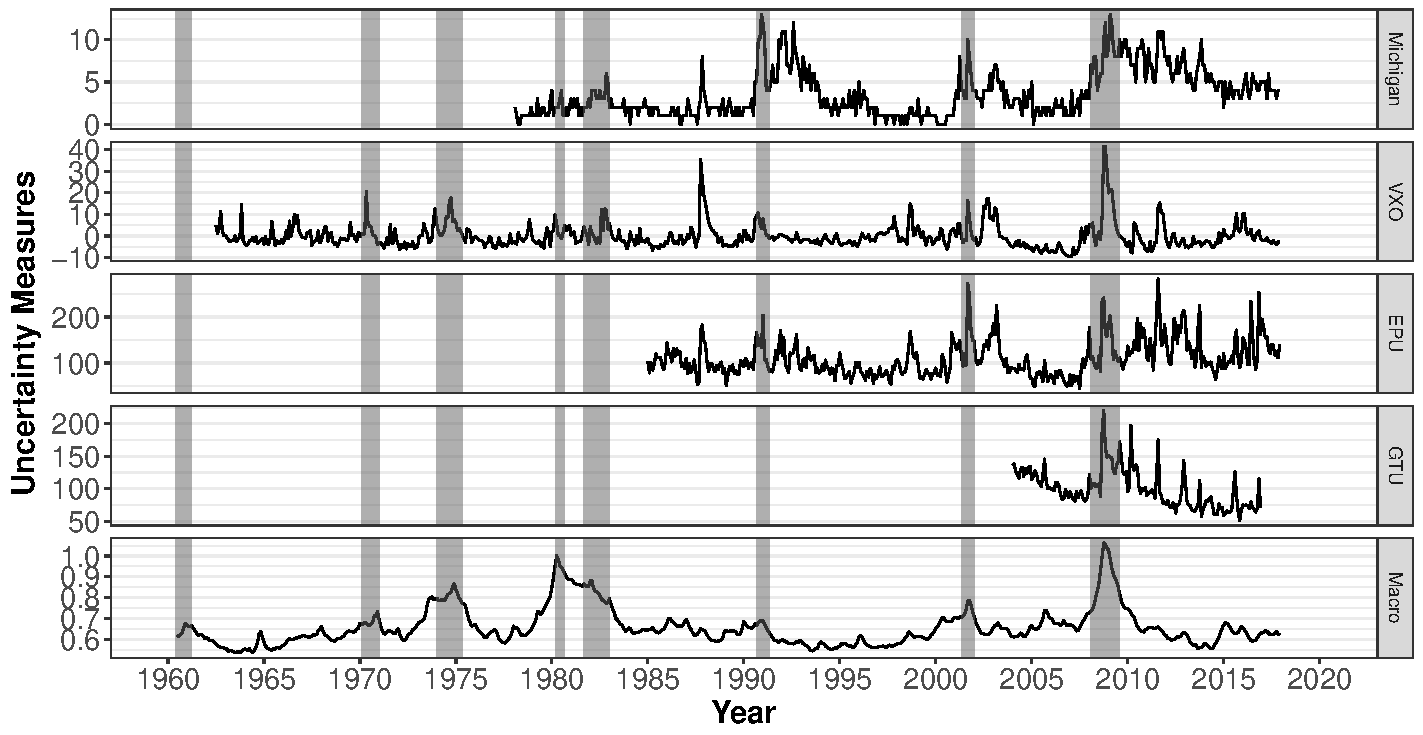
\includegraphics[trim=1cm -1.5cm 0.8cm -0cm, width=0.95\textwidth]{comparison_plot.pdf}}
      \caption[Comparison of uncertainty measures (facetted).]{Comparison of uncertainty measures (facetted).
      \textit{Note:} Shaded areas denote NBER recession dates. Data frequencies are monthly. The macro uncertainty series starts in July 1960, the EPU in January 1960 and the VXO in July 1962.}   \label{fig:comparison_plot}
\end{figure}


The macro uncertainty index overall stands out with an overall smoother trajectory and marked spikes that correspond to recessions but also, as aptly formulated by \citet{juradoetal:15} themselves, significant independent variation as compared to the other commonly used uncertainty measures suggesting that ``[...] quantitatively important uncertainty episodes occur far more \textit{in}frequently\footnote{Italics added.} than what is indicated from common uncertainty proxies, but that when they \textit{do} occur, they display larger and more persistent correlations with real activity'' \citep[p. 1181]{juradoetal:15}. This observation can be confirmed by looking at Figures \ref{fig:comparison_plot} and \ref{fig:comparison_plot_combined}\footnote{And also Table~\ref{tab:summary_stats1} which we will discuss below.} where increases in the macro uncertainty estimates are mostly associated with protracted recessions whereas more modest recessions are accompanied with smaller spikes. A period where the macro uncertainty index stands out is the recessionary period from 1980-1982: throughout this episode the index is highly elevated while other measures are comparatively low. The VXO on the other hand also shows spikes outside of recession periods that correspond to events exclusively related to stock-markets (most notably the large spike commonly to as 'Black Monday' (October, 19th 1987) when stock markets experienced their largest single-day percentage decline ever recorded). The macro uncertainty index, however, barely moves around that time. Interestingly, the EPU shows the largest spike surrounding the years 2001-2001 (the dot-com bubble). 

\begin{table}[t]
\centering
\caption[Correlation matrix of uncertainty measures.]{Correlation matrix of uncertainty measures. [check correlation between EPU and Macro! \citet{bakeretal:15}] report a value of 0.42 while we get 0.15!; also, after re-estimation the correlation between VXO and MACRO decreased from 0.63 to 0.53 --> check again!}
\scalebox{1}{ 
	\begin{tabular}{@{\extracolsep{5pt}} lcccc} 
	\toprule
 	& VXO & Macro & EPU \\ 
	\midrule \\[-1.8ex] 
	VXO & $1$ & $0.490$ & $0.530$ \\ 
	Macro & $0.490$ & $1$ & $0.300$ \\ 
	EPU & $0.530$ & $0.300$ & $1$ \\
	\bottomrule
	\end{tabular} 
}
\label{tab:correlations}
\end{table}


Despite an overall co-movement between the series, the identified episodes of substantial variation in the processes' dynamics suggest that ``[t]hese [time series] are clearly not measures of the same [latent] stochastic process [...]'' \citep[p. 31]{orlikandveldkamp:14}.\\

To shed some light on the above statement, we will comparatively discuss a few univariate and multivariate properties of the various uncertainty measures in turn.

\begin{table}[!h]
\tiny
\centering
\caption[Summary Statistics on the Dynamics of Uncertainty Proxies.]{Summary Statistics on the Dynamics of Uncertainty Proxies.\\
\textit{Note:} IP-corr(k) and EMP-corr(k) are the absolute cross-correlation coefficients between a measure of uncertainty and the 12 month moving average of industrial production or employment in manufacturing growth in period $t+k$, i.e., $\text{IP-corr(k)} = |corr(u_t, \Delta \% IP_{t+k}|$ and $\text{EMP-corr(k)} = |corr(u_t, \Delta \% EMP_{t+k}|$. A positive $k$ means uncertainty is correlated with future IP/EMP. Half-lifes are based on estimates from a univariate AR(1) model for each series and calculated as $HL = ln(2)/ln(AR(1).coef)$. The sample for each uncertainty measure is the largest available, starting in July 1962 in the case of VXO, EPU, Macro1 and Macro12.}
\scalebox{1}{  % blows up or reduces the table in its entirety
\renewcommand{\arraystretch}{1.5} % stretches vertically
\resizebox{\textwidth}{!}{%
    \begin{tabular}{l *{6}{d{3.3}} }
        \toprule
        %below multicolumn is necessary so that the effect of dcolumn is not also applied on the column headers!
         &  \multicolumn{1}{c}{VXO} &  \multicolumn{1}{c}{EPU} &  \multicolumn{1}{c}{Macro1} &  \multicolumn{1}{c}{Macro12} &  \multicolumn{1}{c}{Uf} \\ 
         \midrule
         \multicolumn{6}{l}{\textit{Distribution}}\\
         Coeff. of Variation & 0.38 & 0.37 & 0.14 & 0.08 & 0.19 \\
        Skewness (Levels) & 2.02 & 0.77 & 1.67 & 1.61 & 0.69 \\
        Excess Kurtosis (Levels) & 4.17 & -1.21 & 0.23 & -0.08 & -2.57 \\
        Skewness (Change) & 2.07 & 0.48 & 0.75 & -0.9 & 0.13 \\
        Excess Kurtosis (Change) & 12.9 & 3.33 & 0.35 & 0.6 & 2.12 \\
        Shapiro-Wilk (p-value) & 0 & 0 & 0 & 0 & 0 \\
        \midrule
        \multicolumn{6}{l}{\textit{Cyclicality}}\\
        Downturn/Upturn ratios & 1.5 & 1.14 & 1.25 & 1.13 & 1.25 \\
        Downturn/Upturn ratios & 1.59 & 1.33 & 1.72 & 1.58 & 1.15 \\
        IP-corr(0) & -0.42 & -0.33 & -0.65 & -0.62 & -0.51 \\
        IP-corr(-12) & -0.17 & -0.22 & -0.37 & -0.32 & -0.23 \\
        IP-corr(12) & -0.06 & -0.11 & -0.2 & -0.27 & -0.15 \\
        EMP-corr(0) & -0.51 & -0.34 & -0.64 & -0.58 & -0.53 \\
        EMP-corr(-12) & -0.23 & -0.25 & -0.23 & -0.18 & -0.17 \\
        EMP-corr(12) & -0.24 & -0.17 & -0.34 & -0.39 & -0.31 \\
        \midrule
        \multicolumn{6}{l}{\textit{Persistence}}\\
        AR(1) & 0.84 & 0.81 & 0.99 & 0.99 & 0.99 \\
        Half Life & 4.05  & 3.26 & 57.8 & 129 & 129 \\
        \midrule
        \multicolumn{6}{l}{\textit{Stationarity Tests}}\\
        Level Stationary (p-value)\tablefootnote{KPSS-test with $H_0 = \text{(trend/level) stationary}$.} & 0.05 & 0.01 & 0.09 & 0.03 & 0.03 \\        
        Trend Stationary & 0.01 & 0.01 & 0.01 & 0.01 & 0.01 \\
        \bottomrule
    \end{tabular}
    }
}
\label{tab:summary_stats1}
\end{table}



Table~\ref{tab:summary_stats1} reports several summary statistics including key figures regarding the \textit{distribution} of the uncertainty measures, their \textit{cyclicality} and its nexus to the business cycle, \textit{persistence} and whether we have any evidence for non-\textit{stationarity}. The results point at a few stylized facts:

First, none of the measures passes the Shapiro-Wilk test, meaning that their respective distributions are significantly different from the normal distribution. This is in line with the figures on skewness and kurtosis: the distribution of changes in the measures are positively skewed and show excess kurtosis (fat tails), most pronounced for VXO and EPU indicating that there are more extreme values in these series as compared to Macro1 and Macro12. Together, these observations point at tails on the right side of the distribution being longer than the ones on the left (meaning that the majority of the density's mass and the median lies to the left of the means). Similarly to the dynamics of business cycles, the above findings suggest that increases in the uncertainty measures tend to be larger than decreases. In other words, uncertainty increases faster than it decreases \citep{moore:17}. Further, across all uncertainty measures, the VXO and EPU suggest a higher variability (according to the variation coefficients) which is also visible from the visual inspection of Figures \ref{fig:comparison_plot} and \ref{fig:comparison_plot_combined}.

Second, uncertainty appears to be countercyclical. The measures largely show means and variances that are higher during recessions versus expansions. This is further supported by negative contemporaneous correlations of the uncertainty measures with key economic indicators like industrial production and employment in manufacturing. The figures are strongest for the macro uncertainty series (Macro1 and Macro12) while VXO and EPU are more weakly associated with the business cycle. In line with \citet{bloom:14}, uncertainty seems to be higher during recessions.\footnote{The unconditional negative correlations are, of course, uninformative about causation between real activity and uncertainty.}


Third, as persistence seems to be a relevant ingredient of the impact of uncertainty on business cycles (as shown by, among others, \citet{schaal:17} or \citet{juradoetal:15}), the estimated half-life shocks (derived from the AR(1)-coefficients) of Macro1 and Macro12 with 57 and 129 months, respectively, show a much higher persistency than the other uncertainty proxies with approx. 4 months which is ``[...] a finding relevant for theories where uncertainty is a driving force of economic downturns, including those with more prolonged periods of below-trend economic growth'' \citep[p. 1193]{juradoetal:15}.


\section{Exogenous Impulse vs. Endogenous Response}
\label{sec:exoEndoJuradoetal}
Already \citet{bloom:14} mentions that while uncertainty seems to influence business cycles, it also appears to be endogenously increasing during recessions. This issue plays a crucial role in attempts to disentangle the real effects of uncertainty, meaning that uncertainty itself may be a function of the business cycle. In this respect, popularized VARs employed in the literature might not be capable of adequately separating cause and effect.

 \citet{ludvigsonetal:18} identify two issues in the empirical modeling of uncertainty and point at the following shortcomings: First, in a VAR context (results of which in the literature we have reported in Sections~\ref{sec:selectedworkindetail} and \ref{sec:robustnessofeconspecs}; see also Appendix~\ref{sec:VAREquations} for details), the deployed models primarily rely on recursive schemes as an identification strategy which impacts questions of causality and whose justification in terms of ordering due to contemporaneous movement of the variables seems sometimes arbitrary and not well grounded.\footnote{\citet{ludvigsonetal:18} also discuss other commonly used identification schemes: sign restrictions, long-run restrictions, IV estimations, etc. Because of partly ambiguous theoretical signs of the relationships between uncertainty and real activity, the authors conclude that sign restrictions are inappropriate. Similarly they reject IV analysis, stating that it is very difficult to find truly exogenous instruments.} And because of the wide spectrum of uncertainty theories and non-existence of an all-encompassing structural model which do not provide identifying restrictions for empirical work, for \citet[p. 5]{ludvigsonetal:18} the ``[...] question of cause and effect is fundamentally an empirical'' one. Second, picking up the critique mentioned already in Section~\ref{sec:selectedworkindetail}, uncertainty stemming from financial markets might play a different role in business cycles than real economic uncertainty, referring to \citet{ngandwright:13} who find that all the post-1982 recessions have their origins in financial market disturbances and that these recessions come along with distinctly different features as recessions where financial uncertainty plays a subordinate role.\\

To account for these identified issues, \citet{ludvigsonetal:18} suggest a novel identification strategy within an SVAR framework which differentiates between macro and financial uncertainty and which we will present next the context of the empirical analysis in Section~\ref{EconometricModel}.



%%%%%%%%%%%%%%%%%%%%%%%EMPIRICALANALYSIS%%%%%%%%%%%%%%%%%%%%%%%%
%%%%%%%%%%%%%%%%%%%%%%%EMPIRICALANALYSIS%%%%%%%%%%%%%%%%%%%%%%%%
%%%%%%%%%%%%%%%%%%%%%%%EMPIRICALANALYSIS%%%%%%%%%%%%%%%%%%%%%%%%

\chapter{Econometric Model}
\label{EconometricModel}
\citet{ludvigsonetal:18} suggest a novel identification scheme in an SVAR-context in an attempt to empirically solve the ruled out simultaneous feedback of variables inherent to widely used VAR-analyses in the uncertainty-literature. Instead of a point identification the authors formulate economically reasoned restrictions on the shocks generated by the SVAR-system to adequately shrink the set of possible solutions. This chapter hence first sets the stage by discussing the theoretical background regarding (S)VARs and the so-called identification problem in Section~\ref{sec:TheoreticalBackgroundSVARs} followed by a presentation of the econometric framework of \citet{ludvigsonetal:18} which in combination with their selected shock-restrictions leverages the global identification approach of SVARs by means of the structure of orthogonal matrices following \citet{rubioetal:10}  in Section~\ref{sec:econometricframeworkLMN}.

While the authors first considered shock-restricted structural VAR-approach in \citet{ludvigsonetal:18} in the context of an applicatino to the analysis of uncertainty and business cycles (with its first draft from March 2015; latest draft at the time of writing: August 2019; forthcoming in the American Economic Journal: Macroeconomics), the approach itself is generalized in \citet{ludvigsonetal:17} (first draft: December 2016; latest draft at the time of writing: January 2020).

\section[Preliminaries: Theoretical Background on (S)VARs]{Preliminaries: Theoretical Background on (S)VARs\footnote{This entire section draws heavily from various sources including \citet{hamilton:94}, \citet{lutkepohl:05}, \citet{stockwatson:01}, \citet{villaramirez:10}, \citet{kunst:07}, \citet{whelan:16}, \citet{zivot:00}, \citet{foroni:14}.}}
With the seminal work of \citet{sims:80} and his introduction of VARs, they are widely adopted in practice as an alternative to large scale macroeconometric models despite initial controversies with regard to their usage and interpretation \citep{canova:95, canova:95b}. Because VARs can be ``[...] consistent with many causal structures'' \citep[p. 1]{ludvigsonetal:17}, SVARs offer a richer framework by allowing the model to be fully endogenous but need additional assumptions for point identification of the parameters.

\label{sec:TheoreticalBackgroundSVARs}

\subsection{(S)VARs and the Derivation of Impulse Responses}
\label{sec:SVARsDerviationIRFs}
We consider a stable (which implies stationarity) bivariate\footnote{Note that we start with a bivariate, i.e., two-equations-VAR for ease of exposition. As soon as we switch to matrix notation, the case of $n=2$ versus $n>2$ (for a multivariate VAR-system) is negligible.} dynamic stochastic simultaneous equations model in a \textit{structural} VAR (SVAR) representation for the two time series $y_{1t}$ and $y_{2t}$\footnote{In all our following notation we abstract from deterministic regressors (i.e., trend or constant) and exogenous regressors, meaning that we only consider the stochastic part of a DGP.} whereby the time paths of the two time series depend on one lag of each variable and also influence each other contemporaneously (i.e., the two variables are endogenous)\footnote{Hence, the example we start with is a bivariate SVAR($1$).} so that
\begin{equation} \label{eq:svar1}
\begin{split}
	y_{1t} & = a_{01}y_{2t} + a_{11}y_{1t-1} + a_{12}y_{2t-1} + \epsilon_{1t} \\
	y_{2t} & = a_{02}y_{1t} + a_{21}y_{1t-1} + a_{22}y_{2t-1} + \epsilon_{2t}
\end{split}								
\end{equation}
with 
\begin{equation}
\begin{split}
	\vect{\epsilon_t} \thicksim i.i.d \left (  \begin{bmatrix}
    							0 \\
    							0
 							 \end{bmatrix}, \begin{bmatrix}
    							\sigma_{1}^2 & 0  \\
    							0 & \sigma_{2}^2
 							 \end{bmatrix} \right ),
\end{split}								
\end{equation}
meaning that the error terms $\vect{\epsilon_t}$ are exogenous and independent and identically distributed  for $t = 1, \dots, T$, i.e., white noise.\footnote{Note that for the moment we do not yet impose normality of the errors.} A slight rearrangement of Equation~\ref{eq:svar1} gives 
\begin{equation} \label{eq:svar2}
\begin{split}
	y_{1t} - a_{01}y_{2t} + & = a_{11}y_{1t-1} + a_{12}y_{2t-1} + \epsilon_{1t} \\
	y_{2t} - a_{02}y_{1t} +  & = a_{21}y_{1t-1} + a_{22}y_{2t-1} + \epsilon_{2t}
\end{split}								
\end{equation}
or 
\begin{equation} \label{eq:svar3}
\begin{split}
	\begin{bmatrix}
    	1 & -a_{01} \\
    	-a_{02} & 1
 	\end{bmatrix}
	\begin{bmatrix}
    	y_{1t} \\
    	y_{2t}
 	\end{bmatrix} = 
	\begin{bmatrix}
    	a_{11} & a_{12} \\
    	a_{21} & a_{22}
 	\end{bmatrix} 
	\begin{bmatrix}
    	y_{1t-1} \\
    	y_{2t-1}
 	\end{bmatrix} +
	\begin{bmatrix}
    	\epsilon_{1t} \\
    	\epsilon_{2t}
 	\end{bmatrix} 
\end{split}								
\end{equation}
which, in matrix notation, compactly reduces to 
\begin{equation} \label{eq:svar4}
\begin{split}
	\vect{A_0 y_t} = \vect{A_1}\vect{y_{t-1}} + \vect{\epsilon_t}
\end{split}								
\end{equation}
with $\vect{A_0}$ being called the \textit{impact matrix} containing the contemporaneous effects of an increase of each endogenous variable on the other variable, respectively and $\vect{\epsilon_t}$ is a white noise process with
\begin{equation}
\begin{split}
	\mathbb{E}(\vect{\epsilon_t}) &  = \vect{0}  \\
	\mathbb{E}[\vect{\epsilon_t}\vect{\epsilon_{\tau}^'}]  & =     \begin{cases}
      												\vect{\Sigma_\epsilon}, & \text{for}\ t = \tau \\
      												\vect{0}, & \text{otherwise.}
   								  \end{cases}
\end{split}								
\end{equation}

Hence, the elements off the main diagonal are zero, i.e., structural shocks are assumed to be uncorrelated. A VAR in such a structural representation can be translated into its \textit{reduced form} representation, i.e., a standard VAR model (in this case a VAR(1) because we are considering only one lag at the moment), by premultiplying \ref{eq:svar4} with the inverse of the impact matrix $\vect{A_0}$ (assuming that it exists) which gives
\begin{equation} \label{eq:svar5}
\begin{split}
	          \vect{A_0^{-1}}\vect{A_0}\vect{y_t} & = \vect{A_0^{-1}}\vect{A_1}\vect{y_{t-1}} + \vect{A_0^{-1}}\vect{\epsilon_t}     \iff \\
	\iff 						\vect{y_t} & = \vect{B_1}\vect{y_{t-1}} + \vect{u_t}
\end{split}								
\end{equation}
and which eliminates the previous complication due to contemporaneous relationships with $\vect{B_1} = \vect{A_0^{-1}}\vect{A_1} \iff \vect{A_1} = \vect{A_0}\vect{B_1}$ and $\vect{u_t} = \vect{A_0^{-1}}\vect{\epsilon_t} \iff \vect{\epsilon_t} = \vect{A_0}\vect{u_t}$.\footnote{Note that here we are still deriving all results for a bivariate vector autoregression of order 1, i.e., a VAR($1$). For a multivariate system with $n>2$, accordingly, the relationship between each coefficient matrix in reduced form $\vect{B}_j$ and structural form $\vect{A}_j$ is governed by $\vect{B}_j = \vect{A}_0^{-1}\vect{A}_j$.}\\
The reduced form errors $\vect{u_t}$ are linear combinations of the structural errors $\vect{\epsilon_t}$ with the following reduced-form variance-covariance matrix\footnote{Note that in the bivariate case, $\vect{\Sigma_u}$ is a diagonal matrix only if $-a_{01} = -a_{02} = 0$, i.e., only if there is no contemporaneous correlation.}
\begin{equation} \label{eq:svar6}
\begin{split}
 		\vect{\Sigma_u} \equiv \mathbb{E}[\vect{u_t}\vect{u_t^'}] & = \mathbb{E}[(\vect{A_0^{-1}}\vect{\epsilon_t}) (\vect{A_0^{-1}}\vect{\epsilon_t})' ] = \\
								& = \mathbb{E}[\vect{A_0^{-1}}\vect{\epsilon_t} \vect{\epsilon_t}'\vect{A_0^{-1}}'] = \\
								& = \vect{A_0^{-1}}\mathbb{E}[\vect{\epsilon_t} \vect{\epsilon_t}']\vect{A_0^{-1}}' = \\
								& = \vect{A_0^{-1}}\vect{\Sigma_\epsilon}\vect{A_0^{-1}}'
\end{split}								
\end{equation}
The variance-covariance matrix $\vect{\Sigma_u}$ of the reduced-form VAR is assumed to be a symmetric positive definite matrix which, however, may not be a diagonal matrix due to instantaneous correlations between the error-terms. As a consequence, isolated shocks in the components of $\vect{u}_t$ may not be likely. This reduced form VAR (1) is covariance stationary \textit{if and only if} the eigenvalues of $\vect{A_1}$ have modulus less than 1.\\

Abstracting from possible identification schemes for $\vect{A_0^{-1}}$ for the moment (to which we will come back in Section~\ref{sec:strcuturalVARsIdentification}), under the assumption of covariance stationarity (i.e., if neither the mean nor the autocovariance of the process depend on time $t$) of the vector process $\vect{y_t}$, \vect{y_t} (i.e., the reduced form VAR) can be transformed into its vector moving average (VMA($\infty$); also called Wold MA) representation according to the Wold decomposition theorem\footnote{In words, the Wold Theorem states that any covariance stationary process has an infinite order, moving-average representation.} (i.e., there exists a unique mapping) whereby all past values of $\vect{y_t}$ are substituted out which translates Equation~\ref{eq:svar5} into a linear combination of all $\vect{u_t}$'s (reduced-form innovations) over time (whereby the corresponding MA-weights do not depend on time $t$ but only on $j$, i.e., how long ago the shock $\vect{u}$ occurred):
\begin{equation} \label{eq:svar7}
\begin{split}
 			\vect{y_t} & = \vect{\Psi_0}\vect{u_t} + \vect{\Psi_1}\vect{u_{t-1}} + \vect{\Psi_{2}}\vect{u_{t-2}} + \vect{\Psi_{3}}\vect{u_{t-3}} + \cdots = \\
			& = \sum\limits_{k=0}^\infty \vect{\Psi_k}\vect{u_{t-k}}
\end{split}								
\end{equation}
with $\vect{\Psi_0} =\vect{\mathbf{I_2}}$ and $\vect{\Psi_k}$ can be computed recursively via $\vect{\Psi_k} = \sum\limits_{j=1}^k \vect{\Psi_{k-j}\vect{B_j}}$ for $k=1, 2, \dots$.\footnote{The MA representation of a stable (S)VAR($p$) process is not necessarily of infinite order since that coefficients may turn zero as of a certain lag.}

The corresponding \textit{structural} moving average (SMA($\infty$); structural Wold MA) representation of $\vect{y_t}$ is based on an infinite moving average of the \textit{structural} innovations $\vect{\epsilon_t}$ and is obtained by substituting the mapping between structural and reduced form shocks $\vect{u_t} = \vect{A_0^{-1}}\vect{\epsilon_t}$ for all $t$ into Equation~\ref{eq:svar7} so that
\begin{equation} \label{eq:svar8}
\begin{split}
 			\vect{y_t} & = \vect{\Psi_0}\vect{A_0^{-1}}\vect{\epsilon_t} + \vect{\Psi_1}\vect{A_0^{-1}}\vect{\epsilon_{t-1}} + \vect{\Psi_{2}}\vect{A_0^{-2}}\vect{\epsilon_{t-2}} + \vect{\Psi_{3}}\vect{A_0^{-1}}\vect{\epsilon_{t-3}} + \cdots = \\
			& = \sum\limits_{k=0}^\infty \vect{\Psi_k}\vect{A_0^{-1}}\vect{\epsilon_{t-k}} \\
			& = \sum\limits_{k=0}^\infty \vect{\Theta_k}\vect{\epsilon_{t-k}}
\end{split}								
\end{equation}
which means that $\vect{\Theta_k} = \vect{\Psi_k}\vect{A_0^{-1}}$ for $k = 0, 1, \dots$. In particular, it holds that $\vect{\Theta_0}=\vect{A_0^{-1}} \neq \vect{I_2}$ (in contrast to the VAR-coefficient $\vect{\Psi_0}$ shown above).\\

Looking at the SMA($\infty$) representation of our bivariate system 
\begin{equation} \label{eq:svar9}
\begin{split}
	\begin{bmatrix}
    	y_{1t} \\
    	y_{2t}
 	\end{bmatrix} 
	=
%	\begin{bmatrix}
%    	\mu_1 \\
%    	\mu_2
% 	\end{bmatrix} + 
	\begin{bmatrix}
    	\theta_{11}^{(0)} & \theta_{12}^{(0)}\\
    	\theta_{21}^{(0)} & \theta_{22}^{(0)}
 	\end{bmatrix} 
	\begin{bmatrix}
    	\epsilon_{1t} \\
	\epsilon_{2t}
 	\end{bmatrix} + 
	\begin{bmatrix}
    	\theta_{11}^{(1)} & \theta_{12}^{(1)}\\
    	\theta_{21}^{(1)} & \theta_{22}^{(1)}
 	\end{bmatrix} 
	\begin{bmatrix}
    	\epsilon_{1t-1} \\
	\epsilon_{2t-1}
 	\end{bmatrix} + \cdots 
\end{split}								
\end{equation}
shows that the elements of the $\vect{\Theta_k}$ matrices, $\theta_{ij}^{(k)}$, are the dynamic multipliers/impulse responses of $y_{1t}$ and $y_{2t}$ to changes in $\epsilon_{1t}$ and $\epsilon_{2t}$.\\

Generalizing the above SMA($\infty$) representation to time $t+s$
\begin{equation} \label{eq:svar10}
\begin{split}
	\begin{bmatrix}
    	y_{1t+s} \\
    	y_{2t+s}
 	\end{bmatrix} 
	=
%	\begin{bmatrix}
%    	\mu_1 \\
%    	\mu_2
% 	\end{bmatrix} + 
	\begin{bmatrix}
    	\theta_{11}^{(0)} & \theta_{12}^{(0)}\\
    	\theta_{21}^{(0)} & \theta_{22}^{(0)}
 	\end{bmatrix} 
	\begin{bmatrix}
    	\epsilon_{1t + s} \\
	\epsilon_{2t+s}
 	\end{bmatrix} + \cdots +
	\begin{bmatrix}
    	\theta_{11}^{(s)} & \theta_{12}^{(s)}\\
    	\theta_{21}^{(s)} & \theta_{22}^{(s)}
 	\end{bmatrix} 
	\begin{bmatrix}
    	\epsilon_{1t} \\
	\epsilon_{2t}
 	\end{bmatrix} + \cdots 
\end{split}								
\end{equation}
or more compactly to 
\begin{equation} \label{eq:svar8_1}
\begin{split}
 		\vect{y_{t+s}} = 
%		\vect{\mu} + 
		\vect{\Theta_0}\vect{\epsilon_{t+s}} + \cdots + \vect{\Theta_s}\vect{\epsilon_{t}} + \cdots
\end{split}								
\end{equation}
shows that the $\vect{\Theta}$ - matrices consisting of the MA-coefficients hold the structural dynamic multipliers (the impulse responses). In our bivariate example, these impulse responses are
\begin{equation} \label{eq:svar9}
\begin{split}
 		\frac{\partial y_{1t+s}}{\partial \epsilon_{1t}} = \theta_{11}^{(s)}, \frac{\partial y_{1t+s}}{\partial \epsilon_{2t}} = \theta_{12}^{(s)} \\
		\frac{\partial y_{2t+s}}{\partial \epsilon_{1t}} = \theta_{21}^{(s)}, \frac{\partial y_{2t+s}}{\partial \epsilon_{2t}} = \theta_{22}^{(s)}
\end{split}								
\end{equation}
or more compactly 
\begin{equation} \label{eq:svar10}
\begin{split}
 		\frac{\partial \vect{y_{t+s}}}{\partial \vect{\epsilon_{t}}} =  \vect{\Theta_s}
\end{split}								
\end{equation}
meaning that in matrix $\vect{\Theta_s}$ the entry $(i, j)$ shows the impact of a one-unit increase in the $j$th variable's innovation at date $t$ ($\epsilon_{jt}$) on the value of the $i$th variable at time $t+s$ $(y_{i, t + s})$.\\
Subsequently, a plot of the elements $(i, j)$ of the respective structural MA matrices $\{\vect{\Theta_s}\}_{i, j}$ as a function of $s$, i.e., 
\begin{equation} \label{eq:svar10}
\begin{split}
 		\frac{\partial y_{t+s}}{\partial \epsilon_{t}}
\end{split}								
\end{equation}
is the \textit{impulse-response function} that describes the response of $y_{i, t+s}$ to a one-time one-unit impulse in $y_{jt}$ with all other variables dated $t$ or earlier held constant.\\

If we assume contemporaneous relationships among the endogenous variables, the regressors in the SVAR representation are correlated with the error term and hence would result in biased OLS estimates.\footnote{If $\vect{A_0} = \vect{I_n}$ then this is not the case.} Therefore, in econometric applications the VAR in its reduced form representation is being estimated from the data. While the reduced-form VAR is the one being estimated, it is a purely econometric model without any theoretical component and does not say anything about the structure of the economy and hence the reduced-form error terms $\vect{u_t}$ cannot be interpreted as structural shocks.\footnote{Note that in the estimated covariance matrix for $\vect{\hat{\Sigma}_u}$ the respective errors are usually correlated so that shocks to one variable are usually accompanied with a response to other variables.} Rather, the goal is to get back to the structural representation with a diagonal covariance matrix and economic meaning.\footnote{In practice, the error series in reduced-form VARs are usually correlated while in a structural setting correlated reduced-form shocks are broken down into uncorrelated structural shocks that allow a clearer assessment of effects within a model.} Without imposing any further restrictions, however, the parameters in the SVAR, i.e., models with contemporaneous relationships,\footnote{In a model without contemporaneous relationship no identification issues would emerge.} are not identified, i.e., given values of the reduced form parameters $\vect{B_1}$ and $\vect{\Sigma_u}$, it is not possible to uniquely solve for the structural parameters $\vect{A_0}$, $\vect{A_1}$ and $\vect{\Sigma_\epsilon}$. In particular, the knowledge of the impact matrix $\vect{A_0^{-1}}$ would allow to recover $\vect{A_1}$ via $\vect{A_1} = \vect{A_0}\vect{B_1}$ and the structural errors via $\vect{\epsilon_t} = \vect{A_0}\vect{u_t}$ and subsequently the variance covariance matrix of the structural errors $\vect{\Sigma_\epsilon}$.\footnote{In the bivariate case we consider here, at least 1 restriction on the parameters of the SVAR is required to enable the identification of all structural parameters. }


\subsection[Forecast Error Variance Decomposition]{Forecast Error Variance Decomposition\footnote{This chapter draws from, among others, \citet{lutkepohl:10}, \citet{lutkepohl:05}, \citet{lutkepohlkilian:17}, \citet{zivot:00} and \citet{sims:11}.}}
\label{sec:FEVDTheory}
Besides the impulse response analysis, 'variance decomposition' (more precisely: 'forecast error variance decomposition'; FEVD) is another frequently used tool in the analysis-toolkit of (S)VARs. As aptly formulated by \citet{zivot:00}, the idea behind this decomposition is to derive the proportion of variability of the forecast errors for the $h$-step-ahead prediction of the (S)VARs variables (based on information at time $t$) that can be attributed to the respective structural shocks. In other words, the analysis allows to quantify the importance of each shock in a system in explaining the variation in each of the system's variables.  The computation of the FEVD can be directly derived from the $\vect{\Theta_k}$ matrices, $\theta_{ij}^{(k)}$, which are the dynamic multipliers/impulse responses of the SVARs variables to changes in the respective shocks (and which were derived in Section~\ref{sec:SVARsDerviationIRFs}).

In particular, the following holds:\\
For an (S)VAR-process as outlined in Section~\ref{sec:SVARsDerviationIRFs}, the error of the optimal $h$-step-ahead forecast computed at time $t$ for the time $t+h$ for the system is given by 
\begin{equation} \label{eq:FVED1}
\begin{split}
 		\vect{y}_{t+h} - \vect{y}_t(h) = \sum\limits_{k=0}^{h-1} \vect{\Theta}_k\vect{\epsilon}_{t+h-k}
\end{split}								
\end{equation}
With the elements of the $\vect{\Theta_k}$ matrices denoted as $\theta_{ij}^{(k)}$, the $h$-step-ahead forecast error for the $n$-th component (i.e., the $n$-th variable) of the system $\vect{y}_{t}$ is given by 
\begin{equation} \label{eq:FVED2}
\begin{split}
 		y_{n, t+h} - y_{n, t}(h) & = \sum\limits_{k=0}^{h-1} (\theta_{n1}^{(k)}\epsilon_{1, t+h-k} + \cdots + \theta_{nM}^{(k)}\epsilon_{M, t+h-k})\\
						& = \sum\limits_{m=1}^{M} (\theta_{nm}^{(0)}\epsilon_{m, t+h} + \cdots + \theta_{nm}^{(h-1)}\epsilon_{m, t+1}),
\end{split}								
\end{equation}
meaning that the forecast error of the $n$-th component potentially can consist of all innovations. With the innovations $\epsilon_{m,t}$ being uncorrelated and having unit variances, the MSE of $y_{n, t}(h)$ can be conveniently expressed as
\begin{equation} \label{eq:FVED3}
\begin{split}
 		\mathbb{E}(y_{n, t+h} - y_{n, t}(h))^2 & =  \sum\limits_{m=1}^{M} \left((\theta_{nm}^{(0)} )^2+ \cdots + (\theta_{nm}^{(h-1)})^2\right) \\
		& =  \sum\limits_{k=0}^{h-1} (\vect{e}_n^'\vect{\Theta_k}\vect{e}_m)^2
\end{split}								
\end{equation}
where the last expression is said to be the contribution of innovations in variable $m$ to the forecast error variance (or MSE) of the $h$-step-ahead forecast of variable $n$ and the vector $\vect{e}_m$ is the $k$-the column of the identity matrix.

Defining the $h$-step-ahead forecast MSE matrix as
\begin{equation} \label{eq:FVED4}
\begin{split}
 		\text{MSE}[\vect{y}_t(h)] = \sum\limits_{k=0}^{h-1} \vect{\Theta}_k\vect{\Theta}_k^',
\end{split}								
\end{equation}
the diagonal elements are
\begin{equation} \label{eq:FVED5}
\begin{split}
 		\text{MSE}[y_{n,t}(h)] = \sum\limits_{k=0}^{h-1}\sum\limits_{m=1}^{M}\left(\theta_{nm}^{(0)}\right)^2
\end{split}								
\end{equation}
The respective proportions $\rho_{nm,h}$ of the $h$-step-ahead forecast error variance of variable $n$ which is accounted for by the $\epsilon_{mt}$ innovations in the variable $k$ is the ratio
\begin{equation} \label{eq:FVED6}
\begin{split}
 		\rho_{nm,h} = \frac{\sum\limits_{k=0}^{h-1} (\vect{e}_n^'\vect{\Theta_k}\vect{e}_m)^2}{\text{MSE}[y_{n,t}(h)]}
\end{split}								
\end{equation}

Further, in a stationary model, the limit of the FEVD (i.e., as $h \rightarrow \infty$) is the FVED of $y_t$ because the forecast error covariance matrix (or MSPE) converges to the unconditional covariance matrix of $y_t$ \citep{lutkepohlkilian:17}. 


\subsection{SVARs and the Identification Problem}
\label{sec:strcuturalVARsIdentification}
As explained in Section~\ref{sec:TheoreticalBackgroundSVARs}, the identification of $\vect{A_0^{-1}}$ is needed to seamlessly connect the estimated reduced-form VAR with the structural VAR that is of actual interest.

The usual strategy is to first estimate the reduced-form system as in Equation~\ref{eq:svar5}. In the most simple setting of a VAR($1$)-model this amounts to estimating $n^2 + \frac{n(n+1)}{2}$ parameters ($n^2$ for the coefficient matrix $\vect{B_1}$ and $\frac{n(n+1)}{2}$ for the variance covariance-matrix of the reduced-form errors). 

In our bivariate case above, we concluded that we need at least one restriction on the parameters of Equation~\ref{eq:svar4} so that the system of equations becomes solvable since the estimated variance-covariance matrix alone is not enough \citep{ludvigsonetal:17}. Identification schemes include, among others, zero short-run restrictions (known as Choleski identification), sign restrictions, zero long-run restrictions (also called Blanchard-Quah following \citealp{blanchardandquah:89}), etc.

For example, imposing a short-run restriction by assuming that the impact matrix $\vect{A_0}$ is lower triangular with
\begin{equation} \label{eq:svar11}
\begin{split}
 		\vect{A_0} = 	\begin{bmatrix}
    					1 & 0 \\
					-a_{02} & 1
 					\end{bmatrix}
\end{split}								
\end{equation}
i.e., the restriction that $-a_{01}=0$, is sufficient to just identify $-a_{02}$ (from the reduced form covariance matrix $\vect{\Sigma_u}$; shown below) and subsequently results in 
\begin{equation} \label{eq:svar12}
\begin{split}
 		\vect{A_0^{-1}} = \vect{\Theta_0} = 	
					\begin{bmatrix}
    					1 & 0 \\
					a_{02} & 1
 					\end{bmatrix} = 
						\begin{bmatrix}
    						1 & 0 \\
						\theta_{21}^{(0)} & 1
 						\end{bmatrix}
\end{split}								
\end{equation}
for the SMA representation imposing the restriction that the value $y_{2t}$ does not have a contemporaneous effects on $y_{1t}$ while due to $-a_{02} \neq 0$ we would allow for the reverse.\footnote{Triangulization was also originally proposed by \citet{sims:80} as an identification strategy.} The reasoning behind such an identification strategy usually stems from arguments that declare certain variable to be sticky, meaning that they do not respond immediately to certain shocks. Further, we see that the restriction $a_{01}=0$ in the SVAR representation is equivalent to assuming $\theta_{12}^{(0)}=0$ in the SMA, meaning that $\epsilon_{1t}$ has no contemporaneous impact on $y_{2t}$.

With $\vect{A_0}$ being a lower triangular matrix of the above form, further the reduced form VAR errors $\vect{u_t} = \vect{A_0^{-1}}\vect{\epsilon_t}$ become
\begin{equation} \label{eq:svar13}
\begin{split}
 		\vect{u_t} = \begin{bmatrix}
    					u_{1t} \\
					u_{2t} 
 					\end{bmatrix} = 
						\begin{bmatrix}
    						1 & 0 \\
						a_{02} & 1  
 						\end{bmatrix} 
							\begin{bmatrix}
    							\epsilon_{1t} \\
							\epsilon_{2t} 
 							\end{bmatrix} = 
								\begin{bmatrix}
    								\epsilon_{1t} \\
								\epsilon_{2t}+a_{01}\epsilon_{1t} 
 								\end{bmatrix} 			
\end{split}								
\end{equation}
The SVAR representation derived under the above assumption hence establishes a recursive causal ordering (i.e., a cascading causal chain of shocks) which may be computed using the Choleski factorization of the reduced form covariance matrix $\vect{\Sigma_u}$ (the Choleski identification is hence also called recursive identification). In this identification scheme hence the \textit{order} of the variables entering the VAR matters because the variable placed on top is assumed to be the most exogenous and is only affected by a shock to itself. The actual ordering depends on the researcher's own thinking about the most likely propagation chain a shock will adhere to. Further note that establishing that certain shocks having effects only on some variables at a certain point in time is identical to certain \textit{variables} having effects only on some variable at a certain point in time.

Writing down the Choleski factorization of the positive semi-definite matrix $\vect{\Sigma_u}$ gives
\begin{equation} \label{eq:svar14}
\begin{split}
 		\vect{\Sigma_u} & = \vect{P}\vect{P'} \quad \text{with} \\
		\vect{P} & = \begin{bmatrix}
    							p_{11} & 0 \\
							p_{21} & p_{22}
 							\end{bmatrix}
\end{split}								
\end{equation}
with $\vect{P}$ being a lower triangular matrix with $p_{ii} \leq 0, i = 1, 2$\footnote{The distinction between the application of a Choleski decomposition and the triangular factorization, which we will discuss in turn, in the context of VARs is very subtle and is related to whether a (reduced-form) VAR is estimated and the resulting $\vect{\Theta}_j$ impulse responses are simply mechanically orthogonalized which results in the orthogonalized impulses having unit variance or whether, in the context of an SVAR, a triangular factorization as described next is established and $\vect{A}_0$ is chosen in a way which implies a Wold causal ordering which, qualitatively, establishes the same orthogonalized impulse responses as well without, however, necessarily having unit variances for the $\vect{\epsilon}_t$s.}. A closely related variant of the this classical representation of the Cholesky decomposition is the L$\Lambda$L decomposition (triangular factorization) in the form of 
\begin{equation} \label{eq:svar15}
\begin{split}
 		\vect{\Sigma_u} & = \vect{L}\vect{\Lambda}\vect{L'}
\end{split}								
\end{equation}
where $\vect{L}$ is a lower triangular matrix with $1$s along the diagonal and $\vect{\Lambda}$ is a diagonal matrix with non-negative elements
\begin{equation} \label{eq:svar16}
\begin{split}
	\vect{L} =  \begin{bmatrix}
    				1 & 0 \\
				l_{21} & 1 
 				\end{bmatrix}, 
				\vect{\Lambda} = 
					\begin{bmatrix}
    					\lambda_1 & 0 \\
					0 & \lambda_2 
 					\end{bmatrix},
					\lambda_i \leq 0, i = 1, 2
\end{split}								
\end{equation}
whereby the representation of this decomposition is related to the classical notation of the Cholesky decomposition of the form $\vect{PP'}$ via
\begin{equation} \label{eq:svar17}
\begin{split}
	\vect{\Sigma_u} & = \vect{L}\vect{\Lambda}\vect{L}' = \vect{L}\vect{\Lambda}^{1/2}(\vect{\Lambda}^{1/2})'\vect{L}' = (\vect{L}\vect{\Lambda})^{1/2}\left ( (\vect{L}\vect{\Lambda})^{1/2}\right )' \\
				& = \vect{P}\vect{P'}.
\end{split}								
\end{equation}
In other words, the triangular decomposition $\vect{\Sigma_u} = \vect{L}\vect{\Lambda}\vect{L'}$ is obtained from the Choleski decomposition $\vect{\Sigma_u} = \vect{P}\vect{P'}$ by defining a diagonal matrix $\vect{D}$ which has the same main diagonal as $\vect{P}$ and by specifying $\vect{L} = \vect{P}\vect{D^{-1}}$ and $\vect{\Lambda} = \vect{D}\vect{D'}$.

Starting from a reduced from VAR,
\begin{equation} \label{eq:svar18}
\begin{split}
	\vect{y_t} & = \vect{A_1}\vect{y_{t-1}} + \vect{u_t} \\
	\vect{\Sigma_u} & = \mathbb{E}[\vect{u_t}\vect{u_t}']
\end{split}								
\end{equation}
performing the triangular factorization on the covariance matrix $\vect{\Sigma_u}$ and constructing a pseudo SVAR model by premultiplying the reduced form VAR by $\vect{L}^{-1}$ gives
\begin{equation} \label{eq:svar19}
\begin{split}
	\vect{L}^{-1}\vect{y_t} & = \vect{L}^{-1}\vect{B_1}\vect{y_{t-1}} + \vect{L}^{-1}\vect{u_t}
\end{split}								
\end{equation}
which can be rewritten to
\begin{equation} \label{eq:svar21}
\begin{split}
	\vect{A_0}\vect{y_t} & = \vect{A_1}\vect{y_{t-1}} + \vect{\epsilon_t}
\end{split}								
\end{equation}
with $\vect{A_0} = \vect{L^{-1}}$, $\vect{A_1} = \vect{L}^{-1}\vect{B_1}$, $\vect{\epsilon_t} = \vect{L}^{-1}\vect{u_t}$.

Hence, with a proper choice of $\vect{A}_0$, the pseudo structural errors $\vect{\epsilon_t}$ have a diagonal covariance matrix $\vect{\Lambda}$ resulting from 
\begin{equation} \label{eq:svar22}
\begin{split}
	\mathbb{E}[\vect{\epsilon_t}\vect{\epsilon_t}'] & = \vect{L}^{-1} \mathbb{E}[\vect{u_t}\vect{u_t}']\vect{L^{-1}}' = \\
										& = \vect{L}^{-1} \vect{\Sigma_u} \vect{L^{-1}}' = \\
										& = \vect{L}^{-1} \vect{L \Lambda L}' \vect{L^{-1}}' = \\
										& = \vect{\Lambda},
\end{split}								
\end{equation}
meaning that the matrix $\vect{L}^{-1}$ rescales the reduced-form errors to norm $\lambda$ and accounts for (eliminates) the correlation between the reduced-form errors. The $(i, j)$ element of $\vect{\Lambda}$ gives the variance of $u_{ji}$. Ultimately the structural $\vect{A_0}$ - matrix is
\begin{equation} \label{eq:svar23}
\begin{split}
	\vect{A_0} = \begin{bmatrix}
    					1 & 0 \\
					-a_{02} & 1
 					\end{bmatrix} = 
					\vect{L}^{-1} = 
						\begin{bmatrix}
    						1 & 0 \\
						t_{21} & 1
 						\end{bmatrix}
\end{split}								
\end{equation}

The above result can also be seen by the following:\\
Knowing that one way to orthogonalize impulse-responses in a reduced-form VAR with possibly correlated errors in $\vect{\Sigma}_u$ is the Choleski decomposition (which gives rise to the Wold causal ordering), when the reduced-form variance-covariance matrix instead is decomposed in its triangular factorization as $\vect{\Sigma}_u = \vect{L}\vect{\Lambda}\vect{L}'$ and knowing that $\vect{\Sigma_u}  \equiv \mathbb{E}[\vect{u_t}\vect{u_t^'}]= \vect{A_0^{-1}}\vect{\Sigma_\epsilon}\vect{A_0^{-1}}'$ (which is equivalent to $\vect{\Sigma_\epsilon} = \vect{A_0}\vect{\Sigma_u}\vect{A_0}'$), establishes that $\vect{L} = \vect{A}_0^{-1}$ and $\vect{\Sigma_\epsilon} = \vect{\Lambda}$. 
\\
\\
The Wold causal ordering (as one example of restrictions) implied in $\vect{A}_0^{-1}$ being a lower triangular matrix with $diag(\vect{A}_0^{-1}) = 1$ causes the system of equations $\vect{\Sigma}_\epsilon  = \vect{A_0^{-1}}\vect{\Sigma_u}\vect{A_0^{-1}}'$ having a unique solution (at least locally).
\\
\\
It is particularly this mechanical standard Wold-causal ordering of the elements of $\vect{y_t}$ on which the VAR literature often relies to establish the triangular factorization of the reduced-form variance-covariance matrix $\vect{\Sigma_u}$ which, for example, \citet{jorda:05} criticizes. At the same time, \citet[p. 4]{jorda:05} finds that the ``statistical-based structural identification of contemporaneous causal links'' is a difficult venture. The framework of \citet{ludvigsonetal:18} makes a suggestion for this issue where the $\vect{P}$-matrix to orthogonalize the reduced-form disturbances is not mechanically constructed as the Cholesky decomposition of the error covariance matrix (zero short-run restrictions; recursive identification) but rather is obtained from contemporaneous and theory-based restrictions placed on the $\vect{P}$-matrix.


\section[Econometric Framework of \citet{ludvigsonetal:18}]{Econometric Framework of \citet{ludvigsonetal:18}\footnote{Note that the exposition in \citet{ludvigsonetal:18} is based on general work on shock-restricted SVARs in \citet{ludvigsonetal:17}.}}
\label{sec:econometricframeworkLMN}

As outlined in Section~\ref{sec:exoEndoJuradoetal}, \citet[p. 2]{ludvigsonetal:18} ask, first, whether uncertainty is ``primarily a source of business cycle fluctuations or a consequence of them'' and, second, whether models of uncertainty should distinguish between financial and 'real' macroeconomic uncertainty. Their suggested model hence accounts for the distinction between both types of uncertainty and introduces a novel identification strategy that ``allows for simultaneous feedback between uncertainty and real activity'' which the authors achieve by means of two types of \textit{shock-based} restrictions consisting of (as they call them) ``event constraints'' and ``correlation constraints'' within the class of SVAR models. 

\citet{ludvigsonetal:18} point out that the usage of specific events and/or external variables in an attempt to identify shocks is not new. The rationale goes that constructing shock series from the historical reading of political and economic events (the narrative approach) allows the generation of exogenous and accurately measured shocks. \citet{ramey:16}, however, questions both of these assumptions (exogeneity and accurate measurement). The usage of instruments under the assumption of a zero correlation with some shocks and a non-zero correlation with others promises remedy and allows point identification in SVAR-settings. The approach of \citet{ludvigsonetal:18}, however, gets by without any such exogeneity assumptions and without point identification and rather leverages the properties of the model's shocks to adhere to certain a-priori (inequality) conditions to decide whether a solution is permissible or not. Thereby, the authors build on findings of \citet{rubioetal:10} which we will discuss next.

	
	
\subsection{Identification of SVARs: \citet{rubioetal:10}}
\label{sec:observationalEquivalence}
As formulated in \citet{rubioetal:10}, the identification of structural vector autoregressions (i.e., drawing inference from the reduced-form representation back to the underlying structural parameters in SVARs) is at the root of the 'identification problem' which forces researches to come up with additional '\textit{a priori} restrictions'\footnote{Author's italics.}, so-called ``identifying restrictions''\footnote{Author's quotes.}.

In this setting due to the symmetry of the variance covariance matrix $\vect{\Sigma}_u$ and as outlined in Section~\ref{sec:strcuturalVARsIdentification}, only $\frac{n(n+1)}{2}$ different equations are specified and a necessary condition (as a standard criterion for identification) is that further $\frac{n(n-1)}{2}$ restrictions are needed to identify all $n^2$ elements of $\vect{A}_0^{-1}$ with $n$ being the number of endogenoues variables (called the necessary ``order condition'' by \citealp{rothenberg:71}).\footnote{The case of $n=3$ illustrates the problem: $\vect{\Sigma}_u = \vect{A_{0}^{-1}} \vect{A_{0}^{-1}}^'$ results in $$		
		\underbrace{%
		\begin{bmatrix}
    		\sigma_{11} & \sigma_{12} & \sigma_{13} \\
		\sigma_{21} & \sigma_{22} & \sigma_{23} \\
		\sigma_{31} & \sigma_{32} & \sigma_{33}
 		\end{bmatrix}
		%
}_{\text{6 values}} = \underbrace{%
		\begin{bmatrix}
    		a_{11}^0 & a_{12}^0 & a_{13}^0 \\
		a_{21}^0 & a_{22}^0 & a_{23}^0 \\
		a_{31}^0 & a_{32}^0 & a_{33}^0
 		\end{bmatrix}^{-1}
		%
}_{\text{9 unknowns}}
\begin{bmatrix}
    		a_{11}^0 & a_{12}^0 & a_{13}^0 \\
		a_{21}^0 & a_{22}^0 & a_{23}^0 \\
		a_{31}^0 & a_{32}^0 & a_{33}^0
 		\end{bmatrix}^{{-1}'}$$ 
		where 6 equations are not sufficient to solve the system of linear equations consisting of 9 unknowns.}
		
Referring to \citet{rothenberg:71} and the fact that the ``order condition'' is only a necessary condition, \citet{rubioetal:10} investigate under which conditions such models are globally identified and introduce a novel approach to global identification by exploiting the structure of orthogonal matrices. Central to their paper is the following: \\
\\
In line with our own notation, the class of SVARs that \citet{rubioetal:10} study have the general form
\begin{equation} \label{eq:svar_1}
\begin{split}
	\vect{A}_0 \vect{y}_t = \sum\limits_{j=0}^\infty \vect{A}_j\vect{y}_{t-j} + \vect{\epsilon}_t
\end{split}								
\end{equation}
where they assume 
\begin{equation}\label{eq:svar_2}
\begin{split}
	\mathbb{E}(\vect{\epsilon_t}) &  = \vect{0}  \\
	\mathbb{E}[\vect{\epsilon_t}\vect{\epsilon_{\tau}^'}] & = \vect{\Sigma}_\epsilon = \vect{I}_n.
\end{split}								
\end{equation}
Compactly writing $\vect{A}_{+}^' = [\vect{A}_1^', \vect{A}_2^', \dots, \vect{A}_p^']$ and $\vect{x}_{t}^' = [\vect{y}_{t-1}^', \vect{y}_{t-2}^', \dots, \vect{y}_{t-p}^']$, they rewrite their model as
\begin{equation}\label{eq:svar_3}
\begin{split}
	\vect{A}_0 \vect{y}_t =  \vect{x}_t \vect{A}_+ + \vect{\epsilon}_t
\end{split}								
\end{equation}
with the reduced-form representation implied by the structural model being
\begin{equation}\label{eq:svar_4}
\begin{split}
	 \vect{y}_t =  \vect{x}_t \vect{B} + \vect{u}_t
\end{split}								
\end{equation}
with $\vect{B} = \vect{A}_0^{-1}\vect{A}_+$ and $\vect{u}_t = \vect{A}_0^{-1}\vect{\epsilon}_t$ and
	\begin{equation} \label{eq:svar_5}
	\begin{split}
		\mathbb{E}[\vect{u_t}\vect{u_{\tau}^'}] & = 
      												\vect{\Sigma_u} = (\vect{A}_0^{-1}\vect{A}_0^{-1'})
	\end{split}								
	\end{equation}	
The parameters of the structural model being $(\vect{A}_0, \vect{A}_+)$ and of the reduced-form model $(\vect{B}, \vect{\Sigma}_u)$, \citet{rubioetal:10} denote the set of all structural parameters by $\mathbb{P}^S$ and the set of all reduced-form parameters by $\mathbb{P}^R$ and define the function $g: \mathbb{P}^S \to \mathbb{P}^R: g(\vect{A}_0, \vect{A}_+) = (\vect{A}_0^{-1}\vect{A}_+, \vect{A}_0^{-1}\vect{A}_0^{-1'})$ for the relationship between structural and reduced-form parameters.\\
\\
Equipped with this notation, \citet{rubioetal:10} define the important concept of 'observational equivalence' as follows: \\
Following \citet{rothenberg:71}, two parameter points, $(\vect{A}_0, \vect{A}_+)$ and $(\widetilde{\vect{A}_0}, \widetilde{\vect{A}_+})$, are considered \textit{observationally equivalent} $iff$ they both imply the same probability distribution of the data $\vect{y}_t$. For linear Gaussian models as studied by \citet{rubioetal:10}, this turns out to be equivalent to postulating that two parameter points are \textit{observationally equivalent} $iff$ they both have the same reduced-form representation $(\vect{B}, \vect{\Sigma}_u)$. Based on this, \citet{rubioetal:10} revert back to their function $g$ and conclude that it shows that two parameter points $(\vect{A}_0, \vect{A}_+)$ and $(\widetilde{\vect{A}_0}, \widetilde{\vect{A}_+})$ have the same reduced-form representation $iff$ ``there is an orthogonal matrix $\vect{Q}$ such that $\vect{A}_0 = \vect{\widetilde{\vect{A}_0}}\vect{Q}$ and $\vect{A}_+ = \widetilde{\vect{A}_+} \vect{Q}$''. In this context, \citet{rubioetal:10} write down two definitions:
\begin{defi}
A parameter point $(\vect{A}_0, \vect{A}_+)$ is globally identified if and only if there is no other parameter point that is observationally equivalent.
\end{defi}
\begin{defi}
A parameter point $(\vect{A}_0, \vect{A}_+)$ is locally identified if and only if there is an open neighborhood about $(\vect{A}_0, \vect{A}_+)$ containing no other observationally equivalent parameter point.
\end{defi}

Observational equivalence is inherently linked to the identification problem in SVARs which, with respect to the definitions above and \citet{rubioetal:10}'s formulation are ``neither globally nor locally identified''. This situation calls for adequate restrictions on the part of the structural parameters to make a model identifiable. And because observational equivalence is identical to finding an orthogonal matrix $\vect{Q}$ as described above, the set of all $(n \times n)$ orthogonal matrices $\mathbb{Q}_n$ plays a central role in the derivation of the econometric framework of \citet{ludvigsonetal:18} (see Section~\ref{sec:modelSetup}).
	
Besides the concept of 'observational equivalence', \citet{rubioetal:10} introduce a computationally efficient theorem for the generation of random orthogonal matrices which the authors leverage in the context of the imposition of sign restrictions of an estimated SVAR's impulse response functions. While \citet{ludvigsonetal:18} do not impose any sign restrictions on the part of the impulse responses themselves (but introduce constraints on the shocks; see the details in Section~\ref{sec:modelSetup}), they leverage the theorem for the generation of random orthonormal matrices:

\begin{theo}
Let $\widetilde{\vect{M}}$ be an $n\times n$ matrix with each element having an independent standard normal distribution. Let $\widetilde{\vect{M}} = \widetilde{\vect{Q}}\widetilde{\vect{R}}$ be the $QR$-decomposition of $\widetilde{\vect{M}}$ with the diagonal of $\widetilde{\vect{R}}$ normalized to be positive. Then $\widetilde{\vect{Q}}$ has the uniform (or Haar) distribution.
\end{theo}

\citet{ludvigsonetal:18} make use of this theorem\footnote{This is not immediately obvious from the outline in \citet{ludvigsonetal:18}. We became aware of this due to the Matlab-code of their baseline specification (see footnote \ref{ftn:MatlabCodeFootnote}).} because typically the $\vect{QR}$-decomposition of a Gaussian Matrix $\vect{M}$ does not guarantee to result in a uniformly distributed orthogonal matrix if the diagonal elements of $\vect{R}$ are not positive (see e.g. \citealp{edelman:05}).

\subsection{Baseline Model}
\label{sec:modelSetup}
\citet{ludvigsonetal:18} assume the following reduced-form finite order VAR representation and corresponding infinite MA representation given by\footnote{Note that we adapt the notation of \citet{ludvigsonetal:18} in their original contribution to be consistent with our own notation so far.} 
	\begin{equation} \label{eq:svar_ludvig1}
	\begin{split}
		\vect{y_t} & = \sum_{j=1}^{p} \vect{B_j}\vect{y_{t-j}} + \vect{u_t}\\
		\vect{y_t} & = \sum\limits_{k=0}^\infty \vect{\Psi_k}\vect{u_{t-k}},\\
				\vect{u}_t & \thicksim (\vect{0}, \vect{\Sigma}_u), \vect{\Sigma_u} = \mathbb{E}[\vect{u_t}\vect{u_{\tau}^'}] = \vect{P}\vect{\Sigma}_\epsilon\vect{P'} = \vect{P}\vect{I}_n\vect{P'} = \vect{P}\vect{P'}
	\end{split}								
	\end{equation}	
where $\vect{P}$ is the unique lower-triangular Cholesky factor with non-negative diagonal elements. The authors collect the reduced-form parameters into 
	\begin{equation} \label{eq:svar_ludvig21}
	\begin{split}
		\phi = \Big(\text{vec}(\vect{A}_1)', \text{vec}(\vect{A}_2)', \dots, \text{vec}(\vect{A}_p)', \text{vech}(\vect{\Sigma}_u)'\Big)
	\end{split}								
	\end{equation}	
by making use of the $\text{vec}$\footnote{The $vec$-operator takes an $(n \times n$) matrix and stacks the columns into a single vector of length $n^2$.} and $\text{vech}$\footnote{The $vech$ (vector half) - operator takes a symmetric $(n \times n)$ matrix and stacks the lower triangular half into a single vector of length $\frac{d(d+1)}{2}$.} operator.
\citet{ludvigsonetal:18} formulate the innovations $\vect{u}_t$ to be related to the structural-form SVAR shock $\vect{\epsilon}_t$ via an invertible $(n \times n)$ - matrix $\vect{H}$
	\begin{equation} \label{eq:svar_ludvig2}
	\begin{split}
		\vect{u}_t & = \vect{H}\vect{\Omega}\vect{\epsilon}_t \equiv \vect{A}_0^{-1}\vect{\epsilon}_t
	\end{split}								
	\end{equation}	
with
	\begin{equation} \label{eq:svar_ludvig3}
	\begin{split}
		\vect{\epsilon}_t & \thicksim (\vect{0}, \vect{\Sigma}_\epsilon), \vect{\Sigma}_\epsilon = \mathbb{E}[\vect{\epsilon}_t\vect{\epsilon}_\tau^'] = \vect{I}_n
	\end{split}								
	\end{equation}	
meaning that the structural shocks are mean zero with unit variance, serially and mutually uncorrelated, and the matrix $\vect{\Omega}$ is a diagonal matrix with the variance of the shocks in the diagonal entries and the unit effect normalization that $H_{jj} = 1$ for all $j$.
	\begin{equation} \label{eq:svar_ludvi4}
	\begin{split}
		\text{diag}(\vect{H}) = 1, \vect{\Omega} = \begin{bmatrix}
    		\sigma_{11} & 0 & \dots & 0 \\
		0 & \sigma_{22} & 0 & 0 \\
		0 & \vdots & \dots & 0\\
		0 & 0 & \dots & \sigma_{kk}
 		\end{bmatrix}, 
		\sigma_{kk} \geq 0 \forall j
	\end{split}								
	\end{equation}	
Ultimately, the goal is to study the dynamic effects of the structural shocks (the impulse response functions) as given by
\begin{equation} \label{eq:svar_ludvi5}
\begin{split}
 			\sum\limits_{k=0}^\infty \vect{\Theta_k} = \sum\limits_{k=0}^\infty \vect{\Psi_k}\vect{A_0^{-1}}
\end{split}								
\end{equation}
on $\vect{y_t}$. The authors point out that with autoregressive parameters $\vect{B_j}$ being consistently estimated under regularity conditions, the sample residuals $\hatt{\vect{u_t}}(\hatt{\phi})$  are consistent estimates of the reduced-form errors $\vect{u_t}$ and the estimation problem reduces to uniquely identify the impact matrix $\vect{A_0^{-1}}$ from $\hatt{\phi}$. However, at this stage, the model is under-identified because there are nine parameters to be estimated in $\vect{A_0^{-1}}$ while the covariance structure only provides six restrictions.

Central to the framework of \citet{ludvigsonetal:18} is then the following: \\
By definition they have set $\vect{\Sigma}_u = \vect{P}\vect{P}^'$ with $\vect{P}$ being the unique lower-triangular Cholesky factor. By introducing a set $\mathbb{Q}_n$ of $(n \times n)$ orthonormal matrices,\footnote{Note that \citet{rubioetal:10} were referring only to \textit{orthogonal}, not \textit{orthonormal} matrices. Orthonormality implies orthogonality, i.e., orthonormality is stronger by demanding for each basis vector spanning the respective space to have length 1.} any $\vect{A}_0^{-1} = \vect{P}\vect{Q}$ is 'observationally equivalent' (see the explanations in Section~\ref{sec:observationalEquivalence}) given $\vect{\Sigma}_u$ and hence consistent with the reduced form variance-covariance matrix $\vect{\Sigma}_u = \vect{A}_0^{-1}\vect{A}_0^{-1'}$ for any given $\vect{Q} = (q_1, q_2, \dots, q_n) \in \mathbb{Q}_n$. \citet{ludvigsonetal:18} define this set of observationally equivalent $\vect{A}_0^{-1}$ as 
\begin{equation} \label{eq:svar_ludvi6}
\begin{split}
 			\mathcal{A}_0 = \{\vect{A}_0^{-1} = \vect{P}\vect{Q}: \vect{Q} \in \mathbb{Q}_n\}
\end{split}								
\end{equation}
whereby the only restriction that can be imposed at this stage follows from combining the unit effect normalization on $\vect{H}$ with $\sigma_{jj} \leq 0$ so that a unit change in the structural shock $j$ may be interpreated as a standard deviation increase in variable $j$. Taking this into account, $\mathcal{A}_0$ becomes
\begin{equation} \label{eq:svar_ludvi7}
\begin{split}
 			\vect{\mathcal{A}}_0 = \{\vect{A}_0^{-1} = \vect{P}\vect{Q}: \vect{Q} \in \mathbb{Q}_n, \quad \text{diag}(\vect{A}_0^{-1}) \geq 0\}.
\end{split}								
\end{equation}
By collecting the reduced form innovations $\vect{u}_t$ into $\phi$, \ref{eq:svar_ludvi7} can be written as 
\begin{equation} \label{eq:svar_ludvi8}
\begin{split}
 			\hatt{\mathcal{A}}_0(\phi) = \{\vect{A}_0^{-1} = \vect{P}\vect{Q}: \vect{Q} \in \mathbb{Q}_n, \quad \text{diag}(\vect{A}_0^{-1}) \geq 0\}.
\end{split}								
\end{equation}
Without any further restrictions, $\hatt{\mathcal{A}}_0(\phi)$ contains infinitely many solutions. \citet{ludvigsonetal:18} hence introduce additional restrictions that go beyond classical sign restrictions, or more generally inequality restrictions (which tend to place these restrictions on the impulse response functions and/or $\vect{A}_0^{-1}$ itself) in an attempt to yield a smaller solution set denoted as $\overline{\mathcal{A}_0}(\phi)$.\\
\\
Denoting the collection of zero restrictions imposed on the model as $FZ(\vect{Q}; \phi)$ as in \citet{rubioetal:10}, the novel restrictions that \citet{ludvigsonetal:18} define to create a credible identification scheme involve the \textit{identified structural shocks} $\vect{\epsilon}_t$ either on their own by defining event constraints $FE(\vect{Q}; \phi; \vect{y}_t, \tau^*, \overline{k})$ or in combination with external variables as component correlation constraints denoted $FC(\vect{Q}; \phi, \vect{y}_t, \vect{S}, \overline{\lambda})$. Thereby the set $\hatt{\mathcal{A}}_0(\phi)$ is diminished accordingly.

\citet{ludvigsonetal:18} also contrast their non-Bayesian approach to work which has been done on sign-restricted SVARs in a Bayesian context that also draws random orthogonal matrices $\vect{Q}$ in the course of the $\vect{QR}$-decomposition (see Sections~\ref{sec:solutionAlgorithm} and \ref{sec:observationalEquivalence}) and clarify that these approaches focus on restrictions placed on the sign of IRFs while their approach concentrates on restrictions on the generated shocks. In addition, the authors explain that their approach is frequentist and follows the moment inequality framework of \citet{andrewsandsoares:10} where moment conditions are given by the ``[...] inequalities from the event and correlation constraints, and equalities provided by the covariance structure'' \citet[p. 11]{ludvigsonetal:18}. The $\vect{QR}$-decomposition in their approach is rather of technical nature to generate possible candidates for $\vect{A_0}$.

We will outline these two set of constraints in turn.

\subsubsection{Shock-Based Constraints}
\citet{ludvigsonetal:18} point out that in their setting real activity shocks are considered 'first moment' shocks (which could potentially come from technology, monetary policy, preferences, or fiscal policy innovations). The other two series in the SVAR, financial and macro uncertainty are types of 'second moment' - shocks that could be caused by expected volatility in financial markets or the macro economy, respectively. In this sense, the SVAR-system allows to understand whether shifts on first or second moments (or both) are drivers of business cycles.

\textbf{\textit{Event constraints}}\footnote{Alternatively also called \textit{event inequality constraints}. Concurrent work is \citet{diazramirez:18} where they also suggest shock-restrictions during historical episodes in a Bayesian setting. \citet{ludvigsonetal:17} also reference works by e.g. \citet{cieslakschrimpf:19} and \citet{zeev:18}.} require that identified financial uncertainty shocks have plausible properties during two episodes of heightened financial uncertainty: the 1987 stock market crash and the 2007-09 financial crisis. \citet{ludvigsonetal:18} decide for this constraint because ``a credible identifiation scheme should produce estimates of $\vect{\epsilon}_t$ with features that accord with our ex-post understanding of historical events, at least during episodes of special interest'' \citep[p. 7]{ludvigsonetal:18}.  In particular, event constraints put the bounds $\overline{k}$ on the sign and magnitude of $\vect{\epsilon}_t = \vect{A}_0\vect{u}_t$ during particular episodes which are collected into $\tau^*$. \\
\\
The reason why such special events turn out to be helpful for identification is that, despite the fact that two observationally equivalent structural models $\vect{A}_0^{-1}$ and $\widetilde{\vect{A}}_0^{-1}$ will produce the corresponding shock-processes $\big\{\vect{\epsilon}_t\big\}_{t=1}^T$ and $\big\{\widetilde{\vect{\epsilon}}_t\big\}_{t=1}^T$ where the first and second moments are equivalent, the individual elements of $\vect{\epsilon}_t$ and $\widetilde{\vect{\epsilon}}_t$ are not necessarily equal at each point in time. This can be easily seen because for $\widetilde{\vect{Q}} \neq \vect{Q}$ we get 
\begin{equation} \label{eq:svar_ludvi9}
\begin{split}
\vect{\epsilon}_t & = \vect{A}_0\hatt{\vect{u}}_t = \\
[\vect{A}_0^{-1} & = \vect{P}\vect{Q} \iff \vect{A}_0 = \vect{Q}^{-1}\vect{P}^{-1} \iff \\
\vect{A}_0 & = \vect{Q}^{'}\vect{P}^{-1}] = \\
	& \vect{Q}^'\vect{P}^{-1}\hatt{\vect{u}}_t 
\end{split}								
\end{equation}
and 
\begin{equation} \label{eq:svar_ludvi10}
\begin{split}
\widetilde{\vect{\epsilon}}_t = \widetilde{\vect{A}}_0\hatt{\vect{u}}_t = \widetilde{\vect{Q}}'\vect{P}^{-1}\hatt{\vect{u}}_t = \widetilde{\vect{Q}}\vect{u}_t \neq \vect{\epsilon}_t
\end{split}								
\end{equation}
at any given $t$ which shows that event constraints could be used to reduce the number of solutions in $\hatt{\mathcal{A}}_0(\phi)$ to a smaller set $\overline{\vect{\mathcal{A}}}_0(\phi)$. \\
\\
To show this, \citet{ludvigsonetal:18} consider the bivariate case $n=2$:\\
Writing down
\begin{equation} \label{eq:svar_ludvi11}
\begin{split}
	\begin{bmatrix}
    		u_{1t} \\
		u_{2t}
 		\end{bmatrix} & = 
		\begin{bmatrix}
    			a_{11}^0 &  a_{12}^0 \\
			a_{21}^0 &  a_{22}^0
 			\end{bmatrix}^{-1}
			\begin{bmatrix}
    				\epsilon_{1t} \\
				\epsilon_{2t}
 				\end{bmatrix}  \iff \\
	\begin{bmatrix}
    		\epsilon_{1t} \\
		\epsilon_{2t}
 		\end{bmatrix} & = 
		\begin{bmatrix}
    			a_{11}^0 &  a_{12}^0 \\
			a_{21}^0 &  a_{22}^0
 			\end{bmatrix}
			\begin{bmatrix}
    				u_{1t} \\
				u_{2t}
 				\end{bmatrix} \implies \\
				\epsilon_{1t} & = a_{11}u_{1t} + a_{12}u_{2t}
\end{split}								
\end{equation}
where the values of $u_{1t}$ and $u_{2t}$ are given since data is given for time $t$ in the span $[\tau_1, \tau_2]$. The above example shows that a restriction on the behavior of $\epsilon_{1t}$ at a specific time $t$ results in a non-linear restriction on $\vect{A}_0^{-1}$ and, equivalently, on $\vect{Q}$.
\\
\\
With the stage set according to the above explanations, \citet{ludvigsonetal:18} require $\vect{\epsilon}_t$ to satisfy three event constraints which they parameterize by $\overline{\vect{k}} = (\overline{k}_1, \overline{k}_2, \overline{k}_3)'$\footnote{The bounds will be set below.}, $\overline{\vect{\tau}} = (\overline{\tau}_1, \overline{\tau}_2, \overline{\tau}_3)' = (1987:10, [2007:12, 2009:06], [2007:12, 2009:06])$ and $\vect{y}_t = (U_{Mt}, IPM_{t}, U_{Ft})$ where $U_{Mt}$ denotes macro uncertainty, $IPM_{t}$ a measure of real activity (in this case industrial production in manufacturing) and $U_{Ft}$ a measure for financial uncertainty and collect the constraints into a system of inequalities
\begin{equation} \label{eq:svar_ludvi12}
\begin{split}
	FE(\vect{Q}; \phi, \vect{y}_t, \overline{\tau}, \overline{k}) & = \begin{pmatrix}
	FE_1(\overline{\tau}_1, \overline{k}_1)\\
	 FE_2(\overline{\tau}_2, \overline{k}), \\
	 FE_3(\overline{\tau}_3, \overline{k}_3)
	\end{pmatrix} = \\
	= \begin{pmatrix}
	\sum\limits_{t=1}^T \mathbbm{1}_{t = \overline{\tau}_1= 1987:10} \dot \quad \epsilon_{F\overline{\tau}_1}  \\
	 \sum\limits_{t=1}^T \mathbbm{1}_{t = \overline{\tau}_2 \in [2007:12, 2009:06]} \dot \quad \epsilon_{F\overline{\tau}_2}  \\
	\overline{k}_3
	\end{pmatrix} & - 
	\begin{pmatrix}
	\overline{k}_1\\
	\overline{k}_2  \\
	\sum\limits_{t=1}^T \mathbbm{1}_{t = \overline{\tau}_3 \forall \in [2007:12, 2009:06]} \dot \quad \epsilon_{IPM\overline{\tau}_3} 
	\end{pmatrix} \geq \vect{0}
\end{split}								
\end{equation}
Each $FE_i(\overline{\tau}_i, \overline{k}_i)$ represents a vector of constraints of magnitude $\overline{k}_i$ on $\epsilon_{it}$ for corresponding $t \in \overline{\tau}_i$. Together, $FE(\vect{Q}; \phi, \vect{y}_t, \overline{\tau}, \overline{k})$ defines inequality constraints based on timing, sign and magnitude that help identification of the underlying structural model. $FE_1$ requires that the financial uncertainty shock that occurred in October 1987 be a large one; $FE_2$ postulates that there must be at least one month during the financial crises 2007-2009 for which the financial uncertainty shock was large and positive and $FC_3$ requires that any real activity shocks found during the Great Recession (the NBER dates for the recession coincide with the financial crisis) do not take any unusually large positive values.\\
The motivation for the above constraints is that if a potential $\vect{Q}$ implies a corresponding shock series that is difficult to hold on to during the key time episodes, it will be removed from the solution set $\hatt{\mathcal{A}}_0(\phi)$. Correspondingly, in the postulated inequality constraints the values for the $\overline{k}_i$s have to be meaningful and timing of events $\overline{\tau}_i$ accurate otherwise solutions that pass these constraints will be meaningless after all.
\\
\\
With regard to the first two constraints on financial uncertainty for the stock market crash on Black Monday and the recent financial crisis, \citet{ludvigsonetal:18} declare that the established constraints want to make sure that ``\textit{at least some}\footnote{Author's italics.} of the forecast error variance of $U_F$ in these episodes of most extreme financial uncertainty is attributable to large shocks that originated in financial markets'' which ``is a maintained assumption [...] that we argue is grounded in a broad historical reading of the times'' \citep[p. 8]{ludvigsonetal:18} and here is captured by $\vect{\epsilon}_F$. To clarify, \citet{ludvigsonetal:18} point out that the constraints, however, do not require that all or most of the variability in these episodes should come from shocks originating in financial markets because they do not rule out large adverse shocks in $\vect{\epsilon}_M$ and $\vect{\epsilon}_{IPM}$. 




The second set of constraints considered by \citet{ludvigsonetal:18} are \textbf{\textit{correlation constraints}}\footnote{Alternatively also called \textit{external variable inequality constraints}.} which require that the identified (structural) uncertainty shocks recovered from $\vect{\epsilon}_t = \vect{A}_0\vect{u}_t$ show a minimum absolute correlation (co-movement) with certain variables that are external to the VAR estimations which they denote with $\vect{S}_t$. In their baseline specification they use an aggregate stock market return and impose restrictions on its correlation with uncertainty shocks. \\
\\
As a motivating example, \citet{ludvigsonetal:17} consider the following example of a bivariate reduced-form VAR-model:
\begin{equation} \label{eq:svar_ludvi12_a}
\begin{split}
	\vect{y_t} & = \sum_{j=1}^{p} \vect{B_j}\vect{y_{t-j}} + 
		\begin{pmatrix}
			u_{1t} \\
			u_{2t}
		\end{pmatrix} \iff \\
\vect{y_t} & = \sum_{j=1}^{p} \vect{B_j}\vect{y_{t-j}} + 	
					\begin{pmatrix}
    			a_{11}^0 &  a_{12}^0 \\
			a_{21}^0 &  a_{22}^0
 			\end{pmatrix}^{-1}
		\begin{pmatrix}
			\epsilon_{1t} \\
			\epsilon_{2t}
		\end{pmatrix},\\
		\begin{pmatrix}
			\epsilon_1 \\
			\epsilon_2
		\end{pmatrix} & \thicksim \mathcal{N}(\vect{0}, \vect{I}_n)
\end{split}								
\end{equation}

As already mentioned before, looking at the variance-covariance matrix $\vect{\Sigma}_u$ of the reduced-form residuals $\vect{u_t}$ with $\vect{\Sigma}_u = \vect{A_{0}^{-1}} \vect{A_{0}^{-1}}^'$ which results in 
$$		
		\underbrace{%
		\begin{bmatrix}
    		\sigma_{11} & \sigma_{12} \\
		\sigma_{21} & \sigma_{22}
 		\end{bmatrix}
		%
}_{\text{3 values}} = \underbrace{%
		\begin{bmatrix}
    		a_{11}^0 & a_{12}^0 \\
		a_{21}^0 & a_{22}^0
 		\end{bmatrix}^{-1}
		%
}_{\text{4 unknowns}}
\begin{bmatrix}
    		a_{11}^0 & a_{12}^0  \\
		a_{21}^0 & a_{22}^0
 		\end{bmatrix}^{{-1}'}$$
\citet{ludvigsonetal:17} explain that one more restriction would allow a point identification of the impact matrix $ \vect{A_{0}^{-1}}$. Instead, here \citet{ludvigsonetal:17} assume an external variable $S_t$ which must not necessarily be exogenous (like an adequate instrument would be) due to which it would be contemporaneously correlated with at least one of the structural errors $\epsilon_{1t}$ and/or $\epsilon_{2t}$ (i.e. endogenous). These assumptions translate into $S_t$ being representable by 
	\begin{equation} \label{eq:svar_ludvig1}
		\begin{split}
	S_t =&  \lambda_1 \epsilon_{1t} + \lambda_2 \epsilon_{2t} + \sigma_S \epsilon_{St} \\
	     = & 	\lambda_1 \epsilon_{1t} + \lambda_2 \epsilon_{2t} + Z_t		
	     	\end{split}				
	\end{equation}	
and $e_{St}$ being a shock specific to $S$ which is assumed to be uncorrelated with the structural residuals $e_{1t}$ and $e_{2t}$, respectively. 

In order to exploit the relationship with $S_t$ external to the VAR in the identification of $ \vect{A_{0}^{-1}}$, in their example \citet{ludvigsonetal:17} assume to reject solutions in $\hatt{\mathcal{A}}_0(\phi)$ that, e.g., result in an absolute correlation between $S_t$ and $e_{2t}$ below a certain threshold (i.e. too small). While the expression $\frac{\lambda_2}{\sqrt{\lambda_{1}^2 + \lambda_{2}^2 + \sigma_S{^2}}} = c(\vect{A_0})$ stands for the correlation between $S_t$ and $e_{2t}$ and depends on the particular $\vect{A_0}$ considered, demanding a minimum absolute correlation equals a non-linear constraint between $S_t$ and $e_{2t}$.\\

\citet{ludvigsonetal:18} see their correlation constraints backed by an asset pricing literature that establishes a link between (macro/financial) uncertainty shocks and stock market returns, arguing that these shocks drive the stock market risk premium variation, a leading example being the Capital Asset Pricing Model (see \citealp{sharpe:64, lintner:65}) and variants thereof.\\

To formalize this and further letting $\hat{u}_{St}$ be the first order autoregressive (and orthogonal) residual for $S_t$, $\hat{u}_{St}$, being a reduced-form residual, hence results as a combination of primitive shocks from various sources including, among others, the three shocks modeled within the VAR system (i.e. aggregate stock market returns are assumed to be correlated with the uncertainty shocks), i.e. 
	\begin{equation} \label{eq:svar_ludvig15}
		\begin{split}
S_t = & \lambda_1 \epsilon_{1t} + \lambda_2 \epsilon_{2t} + \lambda_3 \epsilon_{3t} + \lambda_S S_{t-1} + \sigma_S \epsilon_{St} \\
	= &  \lambda_1 \epsilon_{1t} + \lambda_2 \epsilon_{2t} + \lambda_3 \epsilon_{3t} + \lambda_S S_{t-1} +  u_{St}.
	     	\end{split}				
	\end{equation}	

In particular, letting ($c_M(\vect{A}_0)$, $c_{IMP}(\vect{A}_0)$, $c_{F}(\vect{A}_0)$) be the sample correlations between the reduced-form error $\hat{u}_{St}$ of an AR(1)-process estimated for $S_t$ and the structural shocks ($\epsilon_{Mt}(\vect{A}_0)$, $\epsilon_{IPMt}(\vect{A}_0)$, $\epsilon_{Ft}(\vect{A}_0)$) and $\overline{\vect{\lambda}} = (\overline{\lambda}_1, \overline{\lambda}_2, \overline{\lambda}_3)$, \citet{ludvigsonetal:18} establish the following system of inequalities for correlation constraints
\begin{equation} \label{eq:svar_ludvi13}
\begin{split}
	FC(\vect{Q}; \phi, \vect{y}_t, \vect{S}, \overline{\lambda}) & = \begin{pmatrix}
	FC_1(\overline{\lambda}_1 < 0, \vect{S})\\
	 FC_2(\overline{\lambda}_2 \geq 1, \vect{S}), \\
	 FC_3(\overline{\lambda}_3, \vect{S})
	\end{pmatrix} = \\
	& = \begin{pmatrix}
	 		\begin{pmatrix}
	 			\overline{\lambda}_1 - c_M(\vect{A}_0)\\
				\overline{\lambda}_1 - c_F(\vect{A}_0)
			\end{pmatrix} \geq \vect{0} \\
			|c_F(\vect{A}_0)| - \overline{\lambda}_2|c_M(\vect{A}_0| \geq 0 \\
			c_{MF} - \overline{\lambda}_3 \geq 0; c_{MF}^2 = c_M(\vect{A}_0)^2 + c_F(\vect{A}_0)^2.
	\end{pmatrix} 
\end{split}								
\end{equation}
The first and third constraint require that $\epsilon_M$ and $\epsilon_F$ are (sufficiently large) negatively correlated with the external variable $S_t$. In particular, constraint (1) requires that each individual correlation exceed the threshold $\overline{\lambda}_1$ in absolute terms and collectively exceed $\overline{\lambda}_3$. The second constraint requires financial uncertainty shocks to be more highly correlated with the autoregressive residual $e_{St}$ than 'real' (macro) uncertainty shocks bounded by the lower bound $\overline{\lambda}_2$ (which is based on the findings of \citealp{btz:09}). Therefore the authors set the $\overline{\lambda}_2 > 1$. And without fixing the parameterization exactly by which the collective correlation is attributed to $\vect{\epsilon}_{Mt}$ and $\vect{\epsilon}_{Ft}$, respectively, \citet{ludvigsonetal:18} 'only' require that $|c_F(\vect{A}_0)| - \overline{\lambda}_2|c_M(\vect{A}_0| \geq 0 $. The lower bound for the collective correlation between the two uncertainty shocks and $S_t$ is also derived off of the work of \citet{btz:09}.

Together, the constraints in \ref{eq:svar_ludvi13} provide cross-equation restrictions on the parameters in a potential $\vect{A}_0^{-1}$, whereby the correlations are not invariant to orthonormal rotations (by $\vect{Q}$) so that the generated correlations in each draw will be different. 

\subsubsection{Identified Solution Set and maxG - Solution}
Combining default covariance structure restrictions with the introduced event and correlation constraints, \citet{ludvigsonetal:18} call the \textit{identifed}\footnote{Author's italics.} solution set 
\begin{equation} \label{eq:svar_ludvi14}
\begin{split}
\overline{\vect{\mathcal{A}}}_0(\vect{Q}; \phi, \overline{k}, \overline{\tau}, \overline{\lambda}, \vect{S})  = \{\vect{A}_0^{-1} & = \vect{P}\vect{Q}: \vect{Q} \in \mathbb{Q}_n, \quad diag(\vect{A}_0^{-1}) \geq 0\}; \\
			FZ(\vect{Q}; \phi) & = \vect{0}, \\
			FC(\vect{Q}; \phi, \vect{y}_t, \vect{S}, \overline{\lambda}) & \geq \vect{0}, \\
			FE(\vect{Q}; \phi, \vect{y}_t, \overline{\tau}, \overline{k}) & \geq \vect{0}
\end{split}								
\end{equation}
which only contains estimates of $\vect{A}_0^{-1}$ that satisfy all constraints. Thereby a particular solution can only be in both $\hatt{\mathcal{A}}_0$ (the unconstrained solution set) and $\overline{\vect{\mathcal{A}}}_0$ if all restrictions are satisfied. And while $\overline{\vect{\mathcal{A}}}_0$ will be a set as well it should be notably smaller than $\hatt{\mathcal{A}}_0$ (without any additional restrictions other than the usual covariance restrictions).

Both constraints together generate moment inequalities (together with the standard reduced-form covariance restrictions) that produce a reduction of the set of possible model parameters consistent with the data that is large enough to ultimately unambiguously derive most dynamic relationship in the system.\\

The ultimate size of the set $\overline{\vect{\mathcal{A}}}_0$ depends in particular on the chosen thresholds for the values $\overline{k}, \overline{\tau}$ and $\overline{\lambda}$ which we will discuss below.

And while there is no single solution in $\overline{\vect{\mathcal{A}}}_0$ that is more likely than another one, as a reference point (and following \citealp{ludvigsonetal:18}), we will also refer to the so-called 'maxG' - solution when discussing the results. In particular, the 'maxG' - solution serves as a reference point at which the value of the introduced constraints (inequalities) are jointly maximized. Formally, as the maxG-solution the quadratic norm is chosen so that
\begin{equation} \label{eq:svar_ludvi16}
\begin{split}
\vect{A}_0^{maxG} \equiv \operatorname*{argmax}_{\vect{A}_0 \in \overline{\vect{\mathcal{A}}}_0} \sqrt{\overline{f}(\vect{A}_0)^'\overline{f}(\vect{A}_0)} \quad \text{where} \\
\quad \overline{f}(\vect{Q}; \phi, \overline{k}, \overline{\tau}, \overline{\lambda}, \vect{S}) = \begin{pmatrix}
			FZ(\vect{Q}; \phi)' \\
			FC(\vect{Q}; \phi, \vect{y}_t, \vect{S}, \overline{\lambda})' \\
			FE(\vect{Q}; \phi, \vect{y}_t, \overline{\tau}, \overline{k})'	
		\end{pmatrix}^'
\end{split}								
\end{equation}
With respect to the introduced constraints, the inequalities will be large for the most extremely positive financial uncertainty shocks in 1987 and during the Great Recession, for the most negative real activity shocks during the Great Recession and when uncertainty shocks have the highest absolute correlation with the variable external to the VAR (in the baseline case: aggregate stock market returns), both jointly and collectively. With these features, \citet{ludvigsonetal:18} regard the 'maxG' - solution, economically, as the ``worst-case'' - scenario.

\subsubsection{Baseline SVAR(6)-3}
\citet{ludvigsonetal:18} estimate several VAR systems to identify uncertainty shocks from the VAR residuals using the restrictions from above. Here we will reproduce their baseline estimation consisting of $\vect{y}_t = (U_{Mt}, IPM_{t}, U_{Ft})$ where $U_{Mt}$ denotes macro uncertainty, $IPM_{t}$ a measure of real activity (in this case industrial production in manufacturing) and $U_{Ft}$ a measure for financial uncertainty. The VAR-System uses $p=6$ lags. For details on the data we refer to Section~\ref{sec:Data} and Appendix~\ref{sec:dataAppendix}.

\subsubsection{Inference}
\citet{ludvigsonetal:17} point out that their shock-restricted approach in the first place deals with the issue of identification while the issue of inference is yet to be solved. However, to get a sense of the sampling distribution, \citet{ludvigsonetal:17} perform a a Monte Carlo simulation by bootstrapping from the set of shocks $\vect{\epsilon_t}({\vect{A_0}})$ in the \textit{identified set}.


\subsection{Solution Algorithm}
\label{sec:solutionAlgorithm}
As indicated above, a decisive part of the solution algorithm is the construction of the unconstrained solution set $\hatt{\mathcal{A}}_0$ and the derivation of the identified set $\overline{\vect{\mathcal{A}}}_0$. \\
\\
The unconstrained solution set $\hatt{\mathcal{A}}_0$ is obtained through the following steps as outlined in \citet{ludvigsonetal:18}:
\begin{enumerate}[i]
	\item estimation of the reduced-form model and initialization of $\vect{A}_0^{-1}$ as the unique lower-triangular Cholesky factor $\hatt{\vect{P}}$ of $\hatt{\vect{\Sigma}}_u$ with non-negative diagonal elements
	\item rotation of $\hatt{\vect{P}}$ by K = 1.5 million random orthogonal matrices $\vect{Q}$;\\
	 each rotation begins by drawing an $(n \times n)$ matrix $\vect{M}$ of normally and independently distributed values (i.e., drawn from a normal distribution with $\mu = 0$ and $\sigma = 1$); $\vect{Q}$ is then taken to be the orthonormal matrix resulting from a $\vect{Q}\vect{R}$ decomposition of $\vect{M}$
	 \item because $\vect{A}_0^{-1} = \vect{P}\vect{Q}$, the covariance restrictions are imposed by construction 
\end{enumerate}

Every generated $\vect{A}_0^{-1}$ resulting from one of the 1.5 million rotations is then confronted with the event and correlation-constraints for further processing. This step, however, needs a reasonable choice of the parameters $\overline{\vect{\lambda}}, \overline{\vect{\tau}}$ and $\overline{\vect{k}}$. Using a mix of theory, empirical analysis and economic reasoning, \citet{ludvigsonetal:18} set the parameters to  $\overline{\lambda}_1 = -0.05$, $\overline{\lambda}_2 = 2$ and the threshold for the collective correlation to $\overline{\lambda}_3 = 0.18$. The choices for $\overline{k}_1$ and $\overline{k}_2$, are, according to \citet{ludvigsonetal:18} partly guided by \citet{bloom:09} who chooses to study the dynamic effects of four standard deviation shocks to uncertainty in his impulse response analyses. Accordingly, \citet{ludvigsonetal:18} set both $\overline{k}_1 = 4$ and $\overline{k}_2 = 4$.\footnote{This threshold is chosen considering that the shocks are shown to be non-Gaussian with exhibiting excess skewness and kurtosis.} Further, $\overline{k}_3$ is set to 2 to dismiss shocks in real activity that go beyond two standard deviations above their sample mean during 2007-2009.

At each draw of $\vect{A}_0^{-1} = \hatt{\vect{P}}\vect{Q}$ and the subsequent generation of $\vect{\epsilon}_t = \vect{A}_0\hatt{\vect{u}}_t$, the algorithm will only store those models that fulfill all constraints.\footnote{In a fist attempt we had implemented the novel identification strategy of \citet{ludvigsonetal:18} in R by solely following the descriptions in \citet{ludvigsonetal:18} and \citet{ludvigsonetal:17}. Due to some small subleties in the translation of the algorithm's description into code, our resulting trajectories of the impulse response functions as produced by the identified solution set $\overline{\vect{\mathcal{A}}}_0$ were slightly off in this initial attempt as compared to the IRFs reported in \citet{ludvigsonetal:18}. We are hence grateful to Sai Mia, one of the co-authors of \citet{ludvigsonetal:18}, who kindly provided us with their Matlab-code of the baseline-cases to identify the errors.\\
\\
Throughout this exercise we noticed that the authors had computed the variance covariance matrix of the residuals by dividing the residual sum of squares by 652 (the sample size T) while the $var$-package in R applies a degrees of freedom correction via $T-Kp-1 = 652 - 3*6 - 1$ where $K$ stands for the number of variables and $p$ for the number of lags. The applied estimator for the variance-covariance matrix applied by \citet{ludvigsonetal:18} obviously corresponds to the MLE estimator. To be in line with the author's results, we have accordingly applied a correction factor to translate the degrees-of-freedom correction under the OLS-estimation to an MLE-estimator.\label{ftn:MatlabCodeFootnote}}

With the identified set of solutions collected into $\overline{\vect{\mathcal{A}}}_0(\vect{Q}; \phi, \overline{k}, \overline{\tau}, \overline{\lambda}, \vect{S})$ at disposal, the code recursively calculates the coefficients $\vect{\Psi_k}$ (i.e. the MA-weights) of the estimated reduced-form VAR as outlined in Equation~\ref{eq:svar7} from which we subsequently derive the set of SMA-coefficients $\vect{\Theta_k}$ for every respective $\vect{A_{0}^{-1}}$ in the solution set by multiplying all coefficient matrices $\vect{\Psi_k}$ with $\vect{A_{0}^{-1}}$ at every forecast horizon (here: up until 60 steps ahead) as outlined in Equation~\ref{eq:svar8}.

Overall, the combination of event and correlation constraints drastically reduces that possible solution set by about 99\%.


\chapter{Data}
\label{sec:Data}

\citet{ludvigsonetal:18} consider i$\vect{y}_t = (U_{Mt}, IPM_{t}, U_{Ft})$ as the baseline-SVAR-system where $U_{Mt}$ was already mentioned in Section~\ref{sec:uncertaintymeasuresandstylizedfacts}. As a measure of $Y_t$ the log of real industrial production, $ip_t$ is, used. \\

The construction of the uncertainty measures $U_{Mt}$ and $U_{Ft}$ follows the framework \citet{juradoetal:15}. Especially in contrast to stock market volatility and/or cross-sectional dispersion measures frequently deployed in uncertainty studies (see also Section~\ref{sec:uncertaintymeasuresandstylizedfacts}), \citet{juradoetal:15} have designed a computationally and data-intensive approach by making use of a rich set of time series to measure a common component in the time-varying volatilities of forecast errors across a large number of macroeconomic time series.\footnote{Note that, apart from practical issues, \citet[p. 1191]{juradoetal:15} themselves explain the reliance on (most likely revised) ``historical'' data (instead of ``real time'' data) with their goal of forming the ``[...] most historically accurate estimates of uncertainty at any given point in time in [their] sample''.}\\
\\
To set their approach apart from other commonly used uncertainty measures, \citet[p. 1178]{juradoetal:15} argue that ``[...] what matters for economic decision making is not whether particular economic indicators have become more or less variable or disperse \textit{per se}, but rather whether the economy has become more or less \textit{predictable}; that is, less ore more uncertain.''\\
\\
To formalize the rationale behind their approach, they define the $h$-period ahead uncertainty in the variable $y_{jt} \in Y_t = (y_{1t}, \ldots, y_{N_{y}t})'$, denoted by $U^t_{jt}(h)$, as the conditional volatility of the purely unforecastable component of the future value of the series, i.e.,
\begin{equation} \label{eq:juradoetal_1}
U^t_{jt}(h) \equiv \sqrt{\mathbb{E}\Big[(y_{jt+h} - \mathbb{E}[y_{jt+h}|I_t])^2|I_t\Big]},
\end{equation}
where the expectation $\mathbb{E}(\cdot|I_t)$ is taken with respect to information $I_t$ available to economic agents at time $t$. Hence, if the expectation today (conditional on all available information) of the squared error in forecasting $y_{jt+h}$ (i.e. $\mathbb{E}\Big[(y_{jt+h} - \mathbb{E}[y_{jt+h}|I_t])^2|I_t\Big]$) rises, uncertainty in the variable increases. The individual uncertainties at each date are then aggregated into a \textit{macroeconomic uncertainty} index by using aggregation weights $w_j$ as follows:
\begin{equation} \label{eq:juradoetal_2}
U^t_{jt}(h) \equiv plim_{N_{y}\to\infty} \sum_{j=1}^{N_y} w_j U_{jt}^y(h) \equiv \mathbb{E}_w \Big[U_{jt}^y(h)\Big]
\end{equation}

Based on the above definitions, \citet{juradoetal:15} emphasize two features that are central to their approach:
\begin{enumerate}
	\item they distinguish between \textit{uncertainty} in a series $y_{jt}$ and its \textit{conditional volatility} and argue that the proper measurement of uncertainty requires the removal of the entire forecastable component $\mathbb{E}[y_{jt+h}|I_t]$ before the computation of the conditional volatility; without accounting for this, the argument goes, forecastable variation is erroneously classified as ``uncertainty''. According to \citet{juradoetal:15}, this is taken into account only in very few occasions in the literature.\footnote{/citet{orlikandveldkamp:14} }
	\item they claim that macroeconomic uncertainty is ``a measure of the common variation in uncertainty across many series'' and not equal to the uncertainty in any single series $y_{jt}$; \citet{juradoetal:15} see this as an important argument because of uncertainty-based theories of the business cycle that typically require the existence of common (often countercyclical) variation in uncertainty across large numbers of series; \citet{juradoetal:15} hence put their econometric estimation of uncertainty insofar to test, as they expect to find evidence of such an aggregate uncertainty factor common to many series, if the above assumption turns out to be correct.
\end{enumerate}

\begin{figure}[!ht]
   \centering
   \setlength\fboxsep{0pt}
   \setlength\fboxrule{0pt}
   \fbox{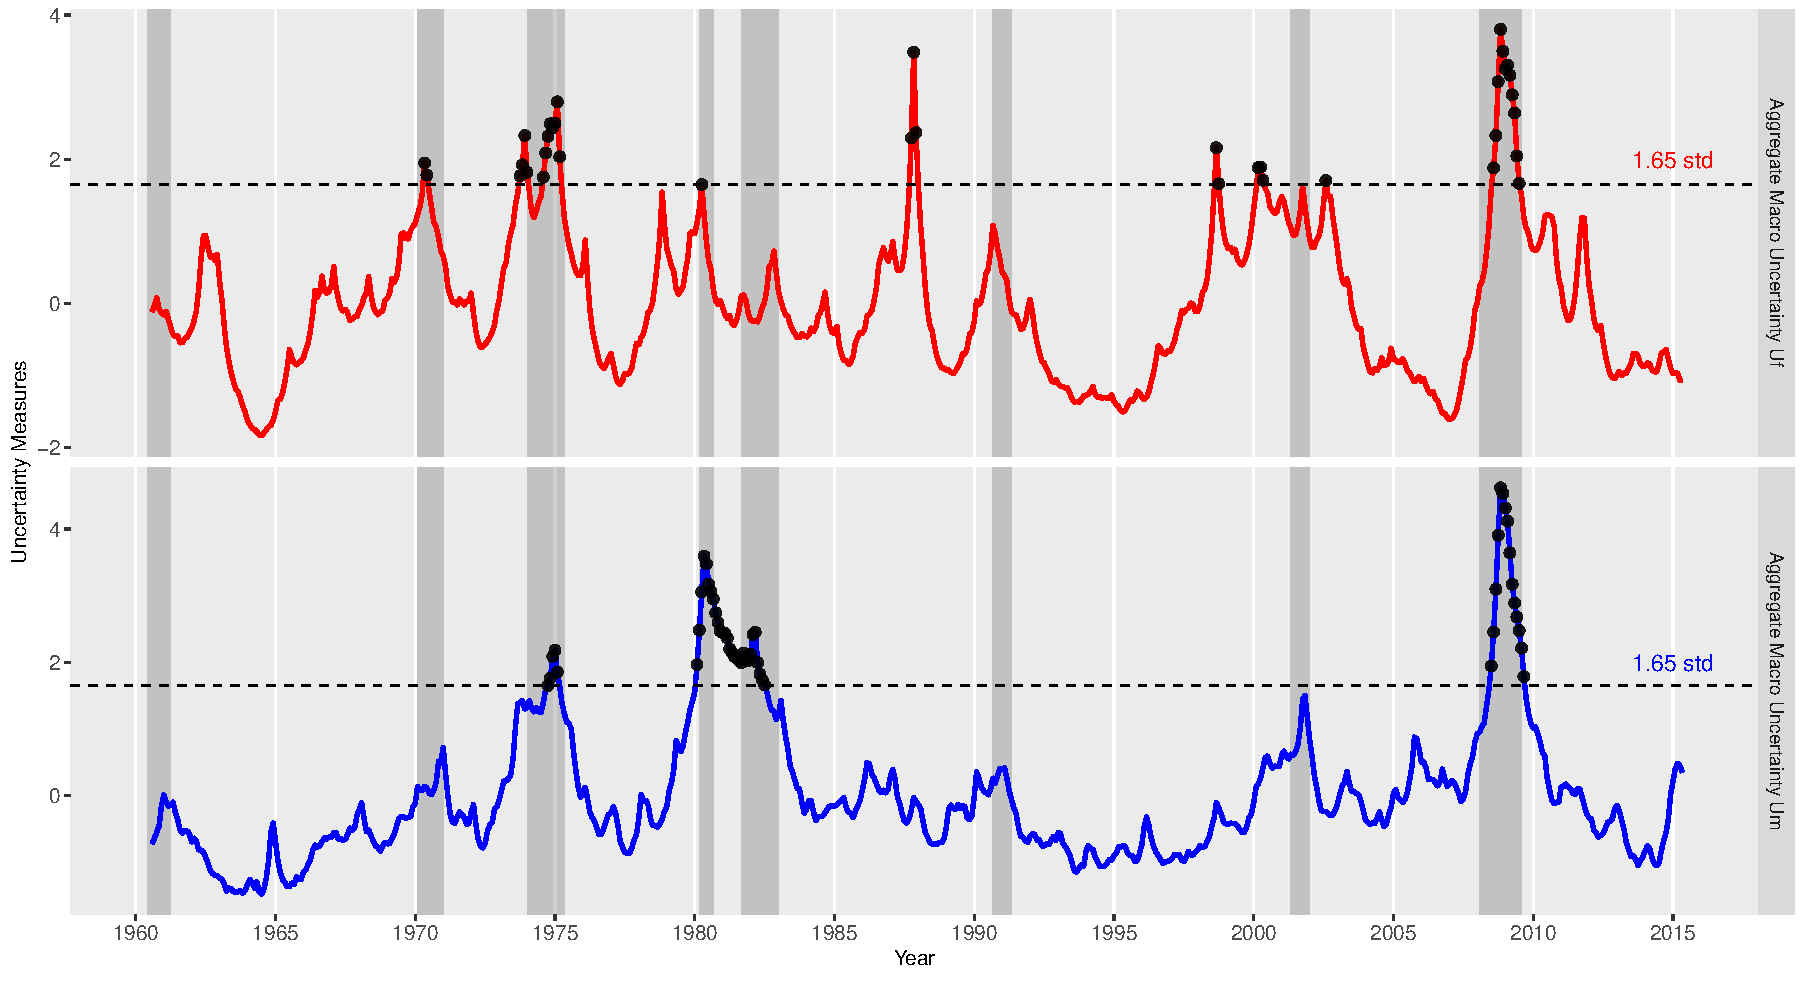
\includegraphics[trim=0cm -2cm 0cm -0.5cm, clip, height=0.6\textwidth, width=1\textwidth]{LMN_Shocks_plot_combined.pdf}}
      \caption[Macro and Financial Uncertainty Over Time.]{Macro and Financial Uncertainty Over Time.
      \textit{Note:} Panels plot the time series of macro uncertainty $U_m$ and financial uncertainty $U_f$ expressed in standardized units. Horizontal lines correspond to 1.65 standard deviations above the unconditional mean of each series (here: normalized to zero). Data are monthly and span the period 1960:7-2015:04. Grey shaded areas denote NBER recession dates in the US.}   \label{fig:macroAndfinUncertainty_index}
\end{figure}

\begin{table}[t]
\centering
\caption{Periods of high uncertainty according to macro uncertainty index h=1.  \textit{Note:} Periods of elevated uncertainty are calculated as months where the value of the respective uncertainty time series is above 1.65 standard deviations of the unconditional mean.}
\scalebox{0.8}{
    \begin{tabular}{ccccc}
    \hline
         Start & End & Duration & Maximum Year/Month & Maximum Value \\ \hline
        Aug 1974 & Feb 1975 & 7 months & Dec 1974 & 0.87 \\
        Dec 1979 & Jul 1982 & 31 months & Apr 1980 & 1.00 \\
        Jun 2008 & Aug 2009 & 14 months & Oct 2008 & 1.06 \\
        \hline
        \hline
    \end{tabular}
}
\label{tab:macro_shocks}
\centering
\end{table}

\begin{table}[t]
\centering
\caption{Periods of high uncertainty according to financial uncertainty index. \textit{Note:} Periods of elevated uncertainty are calculated as months where the value of the respective uncertainty time series is above 1.65 standard deviations of the unconditional mean.}
\scalebox{0.8}{
    \begin{tabular}{ccccc}
    \hline
         Start & End & Duration & Maximum Year/Month & Maximum Value \\ \hline
        Apr 1970 & May 1970 & 1 months & Apr 1970 & 1.23 \\
        Sep 1973 & Dec 1973 & 4 months & Nov 1973 & 1.30 \\
        Jul 1974 & Feb 1975 & 7 months & Jan 1975 & 1.38 \\
        Mar 1980 & Mar 1980 & 1 months & Mar 1980 & 1.18 \\
        Sep 1987 & Nov 1987 & 2 months & Oct 1987 & 1.49 \\
        Aug 1998 & Sep 1998 & 2 months & Aug 1998 & 1.27 \\
        Feb 2000 & Apr 2000 & 3 months & Mar 2000 & 1.22 \\
        Jul 2002 & Jul 2002 & 1 months & Jul 2002 & 1.19 \\
        Jul 2008 & Jun 2009 & 12 months & Oct 2008 & 1.55 \\
        \hline
        \hline
    \end{tabular}
}
\label{tab:fin_shocks}
\centering
\end{table}


The econometric approach then consists of three parts:
\begin{enumerate}[i]
	\item estimation of the forecastable component (conditional expectation) $\mathbb{E}[y_{jt+h}|I_t]$: this is achieved by, first, running a factor analysis on a large set of predictors (134 macro and 148 financial time series, respectively) $\{X_{it}\}, i = 1, 2, \dots, N$ whose linear span/hull comes as close as possible to $I_t$; second, making use of the formed factors, $\mathbb{E}[y_{jt+h}|I_t]$ is then approximated by means of a diffusion index forecasting model ideal for data-rich environments (the diffusion indices can then be treated as known in the subsequent steps)
	\item with the definition of the $h$-step-ahead forecast error as $V_{jt+h}^y \equiv y_{jt+h} - \mathbb{E}[y_{jt+h}|I_t]$, \citet{juradoetal:15} estimate the conditional volatility of this forecast error, i.e., $\mathbb{E}[(y_{jt+h} - \mathbb{E}[y_{jt+h}|I_t])^2|I_t]$ at time $t$ by specifying a parametric stochastic volatility model for both the one-step-ahead prediction errors in $y_{jt}$ and the analogous forecast errors for the factors (from step i above); \\
	these volatility estimates are then used to recursively compute the values of $\mathbb{E}[(V_{t+h}^y|I_t]$ for $h > 1$. 
	\item in the last step, the \textit{macroeconomic uncertainty} index $U_t^y(h)$ is constructed from the individual uncertainty measures $U_{jt}^y(h)$ where the base-case is the equally-weighted average of individual uncertainties
\end{enumerate}

The above approach is applied to 134 mostly macroeconomic time series (taken from \citet{mccrackenandng:16}) for $U_{Mt}$ and to an updated monthly version of 148 financial time series for $U_{Ft}$. Both datasets have been previously used in \citet{ludvigsonandng:07} and \citet{juradoetal:15}. The 134 macro series cover a broad set of macroeconomic time series where the majority are real activity measures like real output and income, employment and hours, etc including a few bond and stock market indices and foreign exchange measures. The 148 purely financial time series  include data from the bond market, stock market portfolio returns and commodity markets. Further details about the exact time-series that are used for the algorithm can be found in \citet{ludvigsonetal:18}.

Their resulting estimated measures of time-varying macro- und financial uncertainty are plotted in Figure~\ref{fig:macroAndfinUncertainty_index}. The macro financial index $U_{Mt}$ reveals 'only' three big episodes of uncertainty: the months during the recessions from 1973-1974 and 1981-1982 and the months during the Great Recession of 2007-2009 (being the most striking episode of heightened uncertainty, followed by the 1981-1982 recession as a close second).\footnote{See Table~\ref{tab:macro_shocks} for the exact dates including the maximum value for the index for each identified episode of high uncertainty.}\footnote{\citet{juradoetal:15} report that a closer look at the estimates reveals that the three series with the highest uncertainty are a producer price index for intermediate materials, a commodity spot price index, and employment in mining between 1973:11 and 1975:3, the Fed funds rate, employment in mining, and the three months commercial paper rate for the 1980:1 and 1982:11 episode and the monetary base, non-borrowed reserves and total reserves between 2007:12 and 2009:6. \citet{juradoetal:15} conclude these results to be consistent with the historical account.} In comparison to $U_{Mt}$, the measure for $U_{Ft}$ shows spikes in times where also $U_{Mt}$ is high but overall is more volatile and spikes more frequently outside of recessions (most notably in October 1987). The exact dates of elevated uncertainty including the maximum value for the index for each identified episode of high uncertainty are reported in Table~\ref{tab:fin_shocks} where the most extreme values are reported in 1987 and 2008.

As shown in Table~\ref{tab:summary_stats1} in Section~\ref{sec:uncertaintymeasuresandstylizedfacts}, the two measures are countercyclical with respect to business cycles (i.e. $ip_t$) with $U_{Mt}$ showing a stronger counter-cyclicality. Overall, as \citet{ludvigsonetal:18} note, the two indicators have comovements but also independent variation (with a correlation coefficient of 0.58). HANS FRAGEN, WAS DIE FORMULIERUNG VON LUDVIGSON ET AL AN DIESER STELLE BEDEUTET: "However, this unconditional correlation cannot be given a structural interpretation. To the extent that our uncertainty variables measure expectations about future volatility, the heightened uncertainty measures can respond endogeneously to events that are expected to happen, but they can also be exogenous changes to expected volatility. We use a VAR to capture the predictable variations, and then identify uncertainty shocks from the VAR residuals using the restrictions described above."







\chapter{Results}
\label{Results}

The complete set of analyses and computations/algorithms for the generation of the results presented in Section~\ref{Results} were conducted in R and follow \citet{ludvigsonetal:18}. Section~\ref{sec:uncertaintyShocks} starts with a preliminary analyses of the behavior of the shocks that are left in the identified set (i.e., passed all shock-restrictions) both for the entire set and, particularly, for the $maxG$-solution and Section~\ref{sec:ImpulseResponseAnalysis} displays and discusses the impulse response analysis. Because there is yet no generally agreed upon method for computing confidence intervals for shock-restricted SVARs in the literature, Section~\ref{sec:EstimatorProperties} relies on bootstrapping/Monte-Carlo following the suggestion of \citet{ludvigsonetal:19} to be able to perform inference in this frequentist setting and, lastly, Section~\ref{sec:FEVD} builds on the IFR-analysis by reporting the results for the forecast error variance decomposition computed over the solutions in the identified set.


\section{Analysis of Recovered Shocks}
\label{sec:uncertaintyShocks}

Before jumping to the resulting impulse responses of the baseline system $\vect{y}_t = (U_{Mt}, IPM_{t}, U_{Ft})$ in Section \ref{sec:ImpulseResponseAnalysis}, Section~\ref{sec:uncertaintyShocks} discusses the SVAR's recovered shocks which are rarely analysed although they are a central objective of SVAR analysis (as formulated by \citealp{ludvigsonetal:17}). These shocks exhibit a few noteworthy features.\\


\begin{figure}[!h]
   \centering
   \setlength\fboxsep{0pt}
   \setlength\fboxrule{0pt}
   \fbox{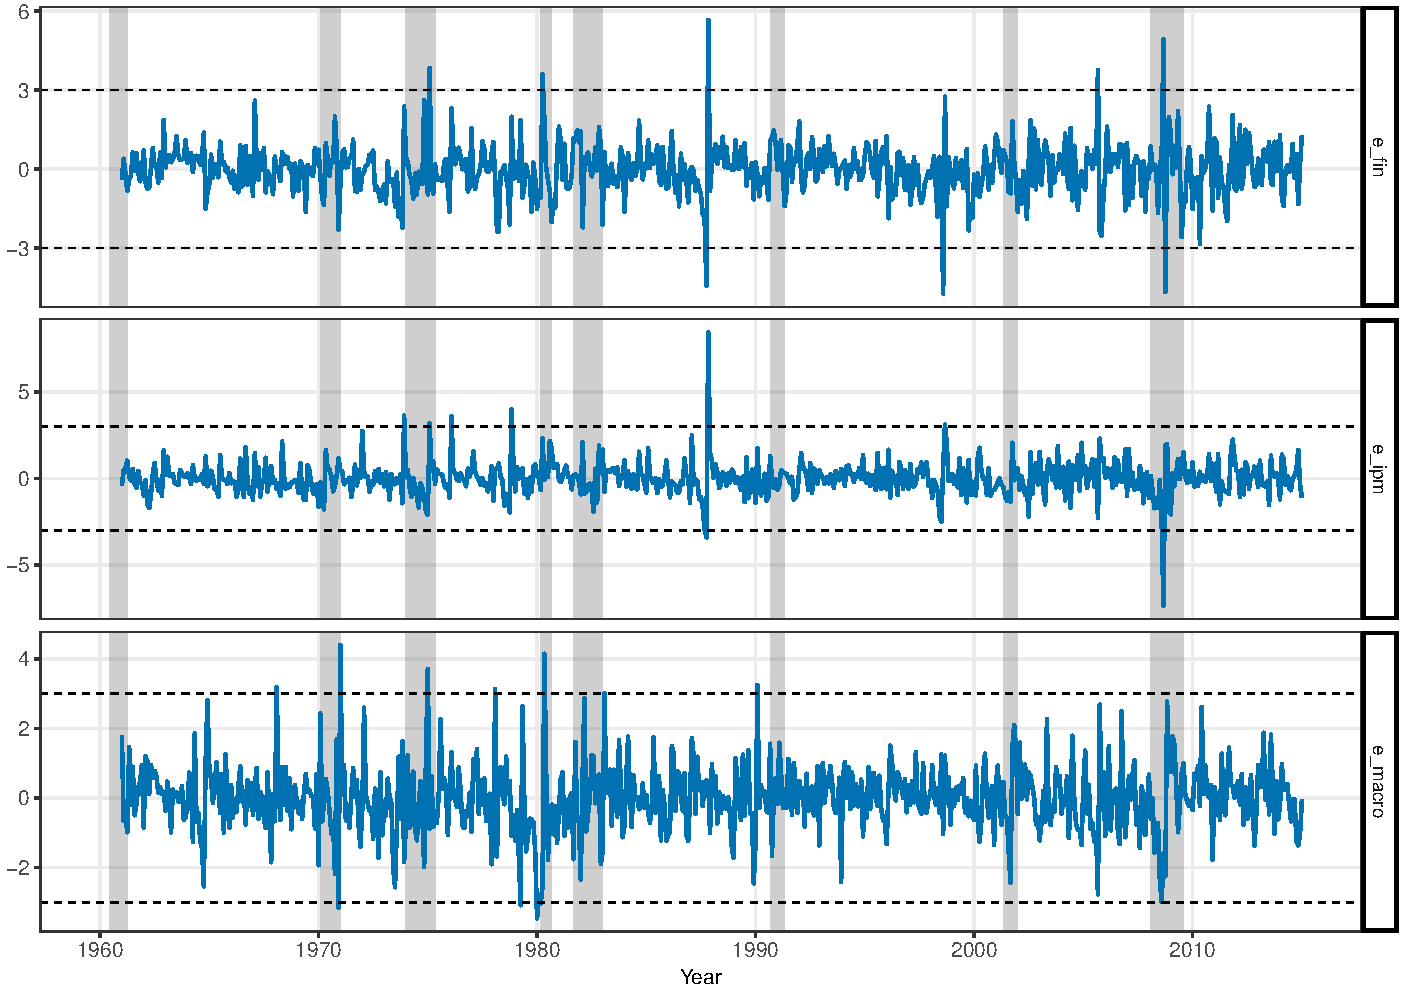
\includegraphics[trim=0.0cm -2.0cm -0.0cm -00cm, width=1\textwidth]{time_series_epsilon_t_maxG.pdf}}
      \caption[Standardized Structural Shocks from SVAR ($U_{Macro}, IPM, U_{Fin}$).]{Standardized Structural Shocks from SVAR ($U_{Macro}, IPM, U_{Fin}$).\\
      \textit{Note:}  The horizontal line corresponds to 3 standard deviations above/below the unconditional mean of each series. The shocks $\vect{\epsilon}_t = \vect{A}_0\vect{u}_t$ for maxG solution are reported, where $\vect{u}_t$ holds the residuals from VAR(6) of ($U_{Macro}, IPM, U_{Fin}$). The selected bounds are $\overline{\lambda}_1 = -0.05$, $\overline{\lambda}_2 = 2$, $\overline{\lambda}_3 = 0.18$, $\overline{k}_1 = 4$, $\overline{k}_2 = 4$, $\overline{k}_3 = 2$. Grey shaded areas denote NBER recession dates in the US}   \label{fig:ludvigsonetal_timeseries_e_shocks}
\end{figure}

Figure~\ref{fig:ludvigsonetal_timeseries_e_shocks} shows that the extracted shocks display pronounced departures from normality. For $e_{lip}$ the largest positive shocks are recorded in 1975:01 and 1971:01, while the largest negative shock is recorded in 1980:04 and 1979:04. For the post-1983-period a moderation in the volatility of the shocks is noteworthy. The two largest positive shocks of $e_{M}$ are in 1970:12 and 2008:10, while for $e_{F}$ they occur in 2008:09 and 1987:10. The time series for $e_{F}$ shows the 1987 stock market crash with a very large spike upward in 1987:10, followed by an even larger downward-spike showing the market's quick recovery. For \citet{ludvigsonetal:18} it is notable that several spikes for both of the two types of uncertainty do not coincide with elevated values for $e_{lip}$ and vice versa.




\begin{figure}[!h]
   \centering
   \setlength\fboxsep{0pt}
   \setlength\fboxrule{0pt}
   \fbox{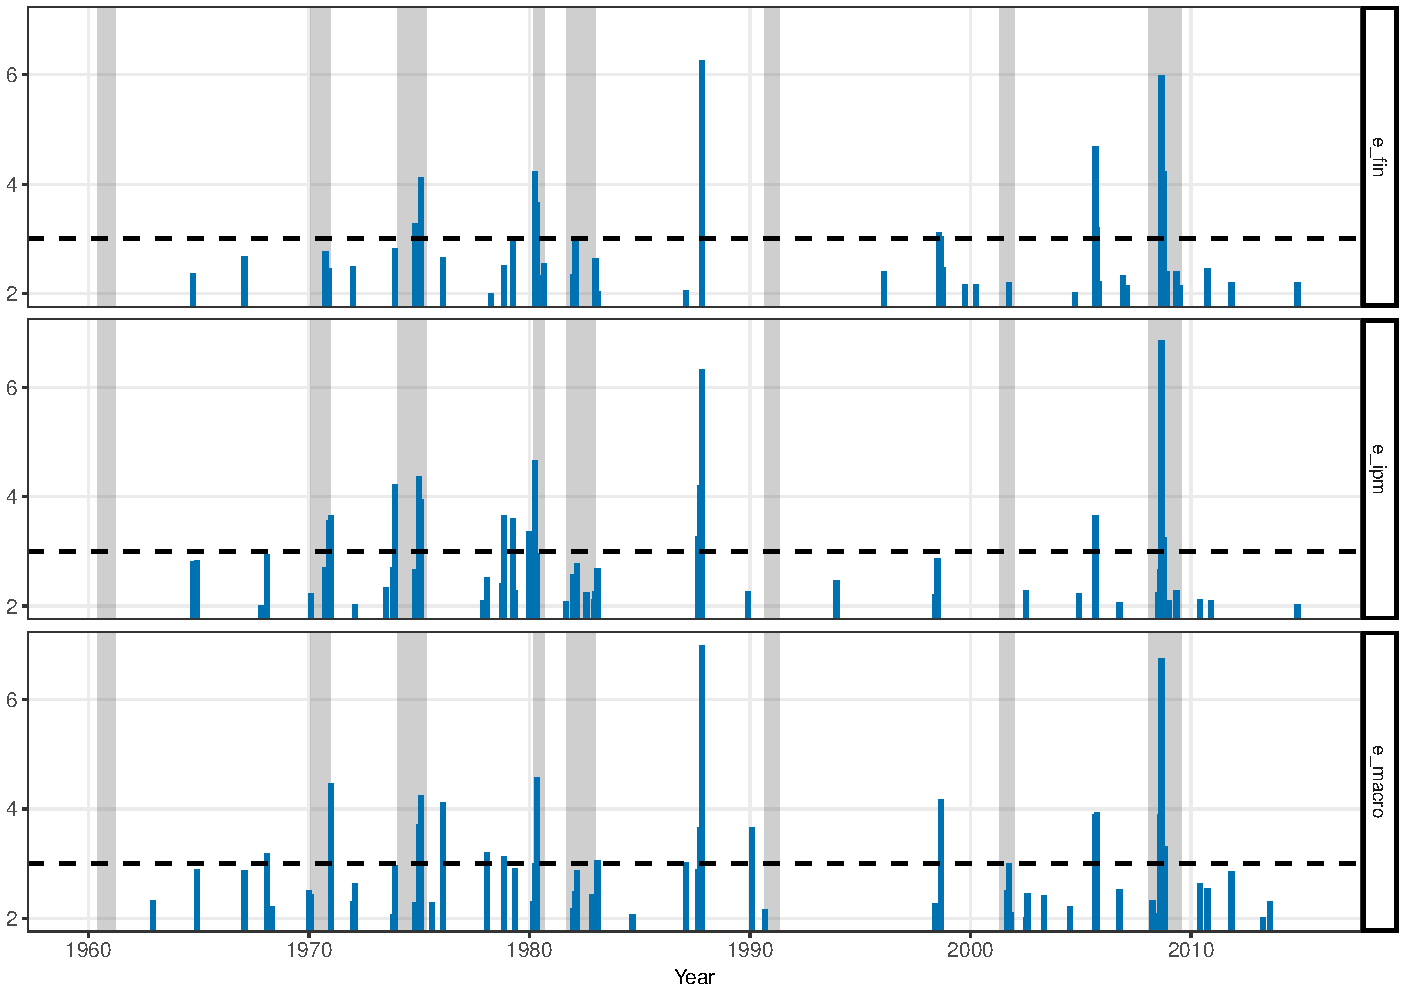
\includegraphics[trim=0.0cm -2.0cm -0.0cm -1cm, width=1\textwidth]{time_series_epsilon_t_largeShocks.pdf}}
      \caption[Large Shocks derived from SVAR ($U_{Macro}, IPM, U_{Fin}$).]{Large Shocks derived from SVAR ($U_{Macro}, IPM, U_{Fin}$).\\
      \textit{Note:}  The figure shows all shocks in the identified set that are at least 2 standard deviations above the unconditional mean for $\epsilon_{Macro}$ and $\epsilon_{Fin}$ and at least 2 standard deviations below the mean for $\epsilon_{ipm}$. For the middle pane ($\epsilon_{ipm}$) the sign of the shocks were flipped (so that negative shocks exceeding 2 standard deviations also point upwards). The horizontal line corresponds to 3 standard deviations. The selected bounds are $\overline{\lambda}_1 = -0.05$, $\overline{\lambda}_2 = 2$, $\overline{\lambda}_3 = 0.18$, $\overline{k}_1 = 4$, $\overline{k}_2 = 4$, $\overline{k}_3 = 2$. Grey shaded areas denote NBER recession dates in the US}   \label{fig:ludvigsonetal_timeseries_e_largeshocks}
\end{figure}

Focussing on large ``adverse'' shocks (large positive uncertainty shocks and large negative real activity shocks recovered by the SVAR-model), Figure~\ref{fig:ludvigsonetal_timeseries_e_largeshocks} shows the date and size of shocks to $e_M$ and $e_F$ that are at least two standard deviations above the mean and negative shocks to $e_{lip}$ that exceed two standard deviations. Contrary to Figure~\ref{fig:ludvigsonetal_timeseries_e_shocks} that only showed the time series for the maxG-solution, Figure~\ref{fig:ludvigsonetal_timeseries_e_largeshocks} shows the resulting large shocks for all solutions that ended up in the identified set. As pointed out be \citet{ludvigsonetal:18}, the top panel which shows large financial uncertainty shocks exhibits the largest spikes in 1987 and 2008. An inspection of large negative shocks for $e_{lip}$ shows that the majority of negative real activity shocks align with recessions or are associated with either financial or macro uncertainty. The negative real activity shock in 2005 slightly stands out but according to \citet{ludvigsonetal:18} could be interpreted as a looming sign of the Great Recession. In their analysis of the 10 housing series that constitute the 134 macro time series, \citet{ludvigsonetal:18} report an onsetting sharp decline as of September 2005. Lastly, the bottom panel of Figure~\ref{fig:ludvigsonetal_timeseries_e_largeshocks} shows that the uncertainty shocks for $e_M$ are a bit more scattered an either coincide or appear with a slight delay after big shocks to real activity or financial uncertainty. The picture for $e_M$ also confirms the period of the Great Moderation as of 1983. Interestingly, around the turn of the millennium non of the series exhibits any larger spikes.\\

Overall, the analysis of the model's residuals confirms the identification scheme to having selected reasonable solutions. And while the solutions clearly adhere to e.g. the event constraints for the 1987 crash or the 2007-09 financial crisis, other large shocks are not ruled which can clearly be seen in Figure~\ref{fig:ludvigsonetal_timeseries_e_largeshocks} where also for $e_M$ and $e_{lip}$, many large adverse shocks fall into these periods.





\section[Impulse Response Analysis]{Impulse Response Analysis}
\label{sec:ImpulseResponseAnalysis}

\begin{figure}[!h]
   \centering
   \setlength\fboxsep{0pt}
   \setlength\fboxrule{0pt}
   \fbox{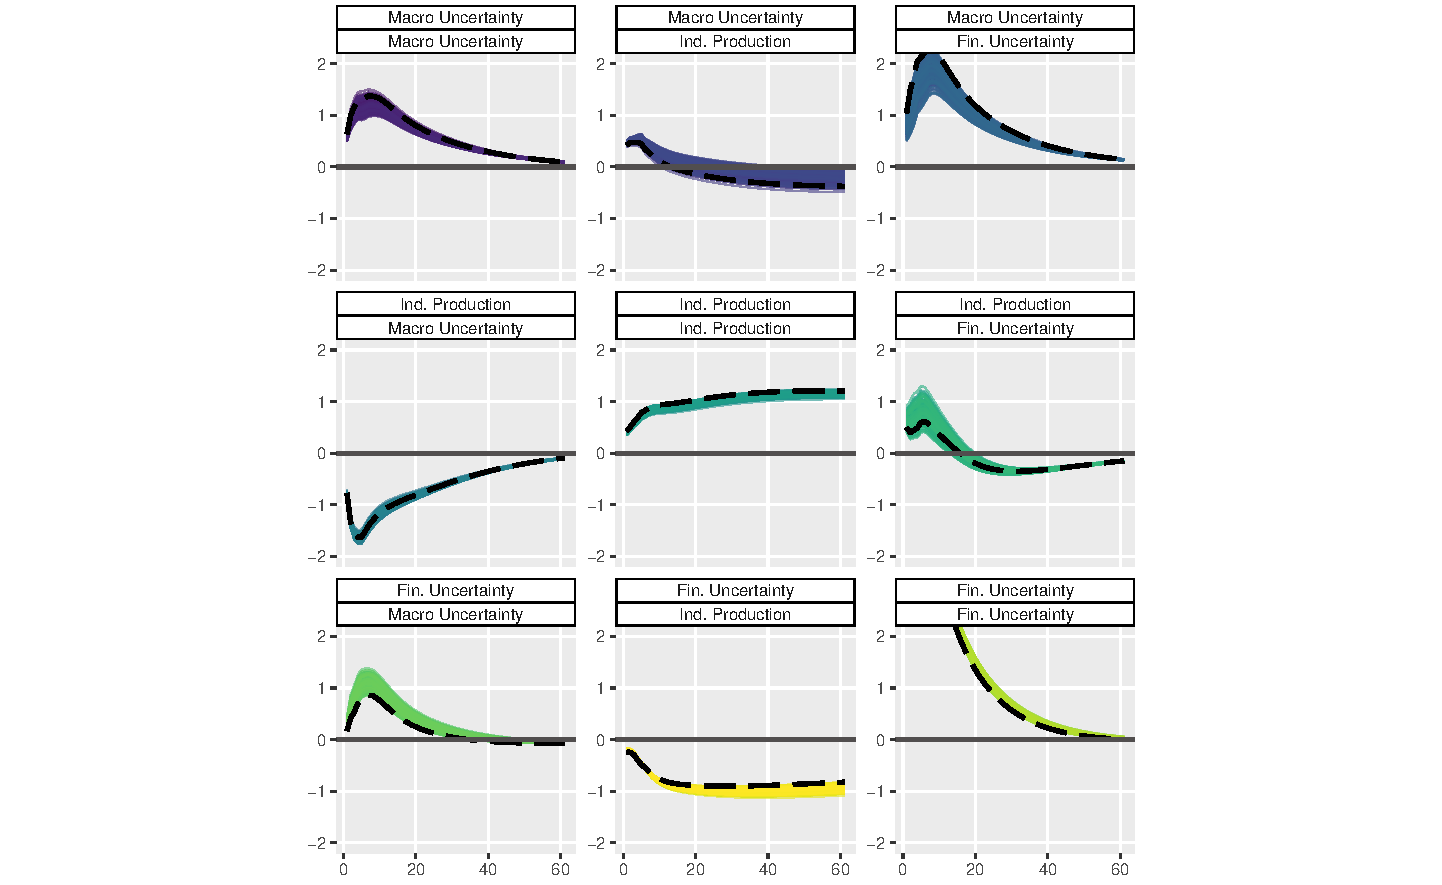
\includegraphics[trim=8cm -1.0cm -6cm -0.5cm, width=1.9\textwidth]{impulse_responses_all_SVAR.pdf}}
      \caption[Impulse Respones from SVAR ($U_{Macro}, IPM, U_{Fin}$).]{Impulse Respones from SVAR ($U_{Macro}, IPM, U_{Fin}$).\\
      \textit{Note:}  The dashed lines are the maxG solutions. The shaded areas represent sets of solutions that satisfy the correlation and event constraints. The selected bounds are $\overline{\lambda}_1 = -0.05$, $\overline{\lambda}_2 = 2$, $\overline{\lambda}_3 = 0.18$, $\overline{k}_1 = 4$, $\overline{k}_2 = 4$, $\overline{k}_3 = 2$. With respect to the labeling, in each panel the bottom label stands for the response of the respective variable to the shock in the top label (the impulse).}   \label{fig:impulse.responses_all.SVAR}
\end{figure}

Having run the algorithm as described in Section~\ref{fig:impulse.responses_all.SVAR}, Figure~\ref{fig:impulse.responses_all.SVAR} shows the set of trajectories of the impulse response functions produced by the impact matrices $A_0$ that passed the set of constraints. Hence, the set of trajectories present the solutions in the identified set that shows the response of each variable to a 1 standard deviation increase for each of the respective structural shocks and how they are transmitted through the SVAR-system. As stated previously, the constraints eliminate almost 99\% of all possible resulting $A_0$-matrices. For our implementation of the algorithm, exactly xxxxx solutions survived the 1.5 million rotations and ultimately ended up in the solution-set. The impulse responses are computed for 60 steps ahead. For the combination of labels in Figure~\ref{fig:impulse.responses_all.SVAR}, the top label always stands for the respective shock, while the second label stands for the response of the respective variable \textit{to} the respective shock. Hence, the IRF in the second row on the left shows the reaction of macro uncertainty to a shock in $e_{lip}$. The thick dotted line represents the maxG-solution which was defined in Section~\ref{sec:modelSetup}. In our replication exercise, the resulting trajectories match the ones' of the paper of \citet{ludvigsonetal:18} pretty closely. 



For sake of comparison, Figure~\ref{fig:impulse.responses_all.SVAR_UNCONSTR} in the Appendix~\ref{sec:additionalFigures} shows the influence of the respective constraints and how either of the two constraints (event \textit{or} correlation constraint) individually still leave a range of possible solutions to the structural shocks. It is the interplay between both shock-constraints that results in largely conclusive answers for the SVAR-system. 




As pointed out by \citet{ludvigsonetal:18}, the impulse response analysis exhibits the following features: First, looking at the bottom row and the second column shows that positive shocks to financial uncertainty $e_F$ lead to a persistent decline in real activity, while they also cause a sharp increase in $U_{Mt}$. For the former case (reaction of industrial production to a $e_F$-shock), the solution-set is ``[...] bounded well away from zero as the horizon increases'' \citep[p. 19]{ludvigsonetal:18}. With these results, the authors find support for the hypothesis of financial uncertainty being an exogenous impulse leading to a decline in real activity. This Contrary to this conclusion, the model gives little support for the impulse going vice versa, i.e., that negative shocks to the real economy induce a heightened and protracted financial uncertainty. Instead, the panel in the second row, third column shows an initial increase of financial uncertainty to a \textit{positive} production-shock. Put differently, a negative production shock \textit{decreases} financial uncertainty at least initially.




Looking at macro uncertainty, \citet{ludvigsonetal:18} find that positive shocks to real activity induce a sharp decline in macro uncertainty $U_{Mt}$. Put differently, a \textit{negative} shock to industrial production would induce a pronounced and protracted \textit{increase} in macro uncertainty as confirmed by the entirety of solutions in the identified set (which is also well away from zero). 

Lastly, interestingly, the SVAR-system (at least for the majority of the solution set as well as the maxG-solution) results in an \textit{increase} in production in response to a macro uncertainty shock $e_{M}$ which \citet{ludvigsonetal:18} see to be consistent with the growth options theory (first row, second column). For the majority of solutions this effect even persists for the long run. Independently of the duration of this effect, the results do not support the empirical evidence of many other empirical applications that point at shocks to macro uncertainty reducing real activity. Instead, as the discussion in the previous paragraph showed, the effect seems to go from real activity shocks to an increase in macro uncertainty and hence weaken the often stated causal nexus between macro uncertainty being a compounding factor in recessions. 

In summary, the model suggests that higher macroeconomic uncertainty is an endogenous response to shocks to aggregate output while \textit{financial uncertainty} can be seen as a likely source for protracted declines in aggregate output.\footnote{\citet{ludvigsonetal:18} also run their algorithms for a pre-crisis sample for which they report less conclusive answers. In their conclusion this result shows that the 2007-2009 financial crisis was an ``[...] important rare event that can help distinguish the transmission of financial versus real uncertainty shocks'' \citet[p. 25]{ludvigsonetal:18}. We have not repeated this exercise here.}


\section{Inference for IRFs: Bootstrapping/Monte-Carlo}
\label{sec:EstimatorProperties}
As discussed in \citet{ludvigsonetal:18}, while for point-identified models inference can be done both via frequentist confidence intervals or Bayesian credible regions, for \textit{set-identified} SVARs ``no consistent point estimate is available'' \citep{ludvigsonetal:18}. While they mention approaches that have been suggested in the literature (\citet{granzieraetal:18} for sign-restricted SVARs that only impose restrictions on one set of impulse response function using the Bonferroni approach or \citet{gafarovetal:15} that collect the reduced-form model in a $1-\alpha$ Wald ellipsoid which is conservative) and with reference to \citet{lutkepohlkilian:17} who show that existing frequentist confidence sets for set-identified models tend to be too large, they conclude that ``[i]t is fair to say that there exists [yet] no generally agreed upon method for conducting inference in set-identified SVARs, let alone one proven to have correct frequentist coverage properties for shock-restricted SVARs of the type considered'' \citep[p. 10]{ludvigsonetal:17}.

To take into account the sampling error and for studying the properties of the estimator, \citet{ludvigsonetal:18} bootstrap from the shocks of the $\vect{\epsilon}_t(\vect{A_0}^{maxG})$ - solution for their baseline-system from Section~\ref{Results}. 

\section[Invalidity of Recursive Identification Schemes]{Invalidity of Recursive Identification Schemes}
\label{sec:ValidityRecursiveSchemes}
\citet{ludvigsonetal:18} argue that recursive schemes in VAR-settings are ill-equipped to properly study the dynamic effects. Accordingly, their suggested and estimated model from Section~\ref{sec:modelSetup} can be tested to see whether it supports a recursive structure because a-priori it does not rule out such a structure. 

\section[Forecast Error Variance Decomposition]{Forecast Error Variance Decomposition}
\label{sec:FEVD}

\begin{table}[!h]
\tiny
\centering
\caption[Forecast Error Variance Decomposition from SVAR $(U_{Mt}, IPM_{t}, U_{Ft})$ where $U_{Mt}$.]{Forecast Error Variance Decomposition SVAR $(U_{Mt}, IPM_{t}, U_{Ft})$ where $U_{Mt}$.\\
\textit{Note:} Each panel shows the fraction of the $h$-step-ahead forecast-error variance of the variable given in the panel title that is explained by the shock named in the column heading. The row denoted "$h = h_max$" reports the maximum fraction of forecast error variance explained across all VAR forecast horizons $h$. The numbers in brackets represent the ranges for these numbers across all solutions in the identified set. The data are monthly and span the period 1960:07-2015:04.}
\scalebox{1}{  % blows up or reduces the table in its entirety
\renewcommand{\arraystretch}{1.2} % stretches vertically
\resizebox{\textwidth}{!}{%
    \begin{tabular}{l *{4}{d{-1}} }
        \toprule
        %below multicolumn is necessary so that the effect of dcolumn is not also applied on the column headers!
	&  \multicolumn{3}{c}{Fraction variation in $U_m$} \\
         \midrule
         \multicolumn{1}{l}{$h$}  &  \multicolumn{1}{r}{$U_m$ Shock} &  \multicolumn{1}{r}{$ip$ Shock} &  \multicolumn{1}{r}{$U_F$ Shock}\\ 
        1 & [0.00, 0.51] & [0.45, 0.80] & [0.04, 0.29] \\
        12 & [0.01, 0.47] & [0.37, 0.62] & [0.16, 0.49] \\
        $\infty$ & [0.01, 0.51] & [0.36, 0.66] & [0.13, 0.42] \\
        \midrule
        	&  \multicolumn{3}{c}{Fraction variation in $ip$} \\
         \midrule
         \multicolumn{1}{l}{$h$}  &  \multicolumn{1}{r}{$U_m$ Shock} &  \multicolumn{1}{r}{$ip$ Shock} &  \multicolumn{1}{r}{$U_F$ Shock}\\ 
        1 & [0.33, 0.96] & [0.00, 0.62] & [0.01, 0.11] \\
        12 & [0.07, 0.60] & [0.07, 0.71] & [0.20, 0.41] \\
        $\infty$ & [0.02, 0.20] & [0.24, 0.69] & [0.28, 0.60] \\
        \midrule
        	&  \multicolumn{3}{c}{Fraction variation in $U_f$} \\
         \midrule
         \multicolumn{1}{l}{$h$}  &  \multicolumn{1}{r}{$U_m$ Shock} &  \multicolumn{1}{r}{$ip$ Shock} &  \multicolumn{1}{r}{$U_F$ Shock}\\ 
        1 & [0.00, 0.12] & [0.01, 0.10] & [0.82, 0.97] \\
        12 & [0.00, 0.01] & [0.00, 0.04] & [0.84, 0.96] \\
        $\infty$ & [0.00, 0.00] & [0.02, 0.05] & [0.81, 0.92] \\
        \bottomrule
    \end{tabular}
    }
}
\label{tab:FEVD_all}
\end{table}

As formulated in \citet{lutkepohlkilian:17}, another frequently studied property of (S)VAR models is how much of the forecast error variance (alternatively also called prediction mean squared error; MSPE) of a time series variable is accounted for by each structural shock. Based on the derivations in Section~\ref{sec:FEVDTheory} and in line with \citet{ludvigsonetal:18}, Table~\ref{tab:FEVD_all} below reports the computed fraction of the respective $h$-step-ahead forecast error variances which for each of the system's variable can be attributed to the respective shocks $\epsilon_{Mt}$, $\epsilon_{ip}$ and $\epsilon_{Ft}$ for the forecast horizons $h=1$, $h=12$ and $h=\infty$ as well as $h_{max}$ which denotes the forecast horizon where the respective fraction is maximized.









Following \citet{ludvigsonetal:18}, the results in Table~\ref{tab:FEVD_all} report \textit{ranges} for the proportions of the forecast error variances because the computations are performed for every solution in the identified set. The results show that shocks in real activity have pronounced (negative) effects on macroeconomic uncertainty (top panel) while they exert minimal effects on financial uncertainty (bottom panel). \citet{ludvigsonetal:18} state that, surprisingly, shocks to macro uncertainty explain a large proportion of industrial production (and in Section~\ref{sec:ImpulseResponseAnalysis} suggested that they increase real activity in the short run).

Contrary to macro uncertainty or real activity, shocks to financial uncertainty exhibit the largest impact on themselves while they also shock a large negative effect on production for longer horizons. From this observation \citet[p. 28]{ludvigsonetal:19} conclude that $U_{Ft}$ suggest to be ``[...] the most important exogenous impulse in the system.''



%\section[Variance Decomposition]{Variance Decomposition}
%\label{sec:VarianceDecomposition}


%\chapter{Model Extension/Alternative Estimations}
%\label{sec:ModelExtension}
%In comparison to the baseline-SVAR-system of \citet{ludvigsonetal:18}, here we consider an additional system that uses the 'Bloom-shock' (see \citealp{bloom:09}) in place of $U_{Ft}$. \citet{ludvigsonetal:18} themselves declare that their approach of analyzing shocks during selected historical episodes to identify solutions is equivalent to ``[...] creating dummy variables from the timing of specific events, and then putting restrictions on their correlation with the identified shocks'' \citep{ludvigsonetal:18}. Since \citet{ludvigsonetal:18} did not include this approach as an alternative into their robustness checks, we replace their variable for financial uncertainty $U_F$ with the Bloom-shocks (see Appendix~\ref{sec:} for the timing of the respective shocks). 


%\paragraph{Robustness Checks: Alternative Uncertainty Measures}
%This part provides results from a large number of robustness exercises designed to check the sensitivity of our results to various assumptions. (this sentence is formulated like this by \citet{juradoetal:15}).




%\newpage
\chapter{Conclusion}
\label{Conclusion}
Frequently used VARs with recursive schemes in the uncertainty literature might empirically not be well grounded to capture the underlying data's DGP and the system's dynamics by ruling out simultaneous feedback between the variables. In addition, those models usually do not distinguish \textit{types} of uncertainty and using individual proxies one at a time suggest that uncertainty largely has a depressing effect on business cycles.

Within the class of SVAR models that also allow for contemporaneous relationships, economically grounded assumptions for point identification often seem too restrictive to defend which is why alternative identification schemes that \textit{set-identify} \citep{granzieraetal:18} SVARs seem like a promising approach. Besides sign-restrictions one strand of the literature which is being pushed by \citet{ludvigsonetal:17}, among others, goes beyond classical sign restrictions and concentrates on the model's recovered \textit{shocks} that might reveal valuable information for sensible inequality restrictions to shrink an SVAR's infinitely many solutions to a manageable solution set even without point identification. 

While in the presented application of the shock-restricted SVAR-approach of \citet{ludvigsonetal:18} the authors have formulated a-priori shock-restrictions, \citet{ludvigsonetal:17} formulate that writing an SVAR first as a VAR which provides $n(n+1)/2$ restrictions from the covariance structure and subsequent analysis of the unrestricted model's residuals might prove useful to support evidence for the confirmation of historically relevant episodes even \textit{before} any identifying restrictions are imposed.

With respect to the particular application and the central question related to the role of uncertainty in business cycles, the novel approach of \citet{ludvigsonetal:18} questions frequently cited results of the uncertainty-literature to date: the results of the baseline 3-variable SVAR(6)-system indicate that, first, the uncertainty literature should distinguish between macroeconomic and financial uncertainty and their different roles in business cycles and, second, that higher macroeconomic uncertainty is an endogenous \textit{response} to shocks to aggregate output while financial uncertainty can be seen as a likely source for protracted declines in aggregate output. While these initial results are certainly a first start, the above conclusions should serve as a first indication that empirical applications in the uncertainty literature have to be cautious with overly restrictive modeling assumptions that might result in precipitous conclusions.\footnote{Another problem for VAR-system are omitted variables (which are assumed to be in the innovations). If important variables are omitted from the system, this may lead to major distortions in the impulse responses and makes them worthless for structural interpretations (see e.g. \citet{lutkepohl:05}).} \\

From a statistical perspective, \citet{ludvigsonetal:18} themselves point at the challenge of proper inference within the class of \textit{set-identified} models in a frequentist view. While they mention approaches that have been suggested in the literature (\citet{granzieraetal:18} for sign-restricted SVARs that only impose restrictions on one set of impulse response function using the Bonferroni approach or \citet{gafarovetal:15} that collect the reduced-form model in a $1-\alpha$ Wald ellipsoid which is conservative), they conclude that ``[i]t is fair to say that there exists [yet] no generally agreed upon method for conducting inference in set-identified SVARs, let alone one proven to have correct frequentist coverage properties for shock-restricted SVARs of the type considered'' \citep[p. 10]{ludvigsonetal:17}. \\

With regard to the particular \textit{type} it seems generally agreed that uncertainty as a latent and generally unobservable stochastic process seems to be multilayered/manifold. Hence, distinguishing between financial and macroeconomic uncertainty in empirical models seems to be the minimum amount of sophistication. One aspect that we haven't touched upon, however, are aspects related to \textit{policy-induced} uncertainty. This relates particularly to questions of how policies can help overcoming a recession and set counter-cyclical measures once an economy has arrived at the bottom. E.g. \citet[p. 41]{bloometal:13} and \citet{IMF:12} write that while ``[i]t is difficult for policymakers to overcome the intrinsic uncertainty economies typically face over the business cycle'', uncertainty about economic policy seems like an exacerbating factor. Hence, we propose to include economic policy uncertainty as a third layer of uncertainty into future structural models since it seems to play another role which should be distinctively separated from macroeconomic and financial uncertainty. \\

Lastly, at the time of writing this thesis the world is halting in the wake of the Covid-19 pandemic which from a global health crisis simultaneously turned into (most likely) the most severe economic decline since the Great Depression due to the necessary lockdown measures applied by governments throughout the world. In context of our uncertainty-taxonomy introduced in Section~\ref{introduction} it is difficult to decide for a classification since on the one hand this external shock might be described as the 'highly improbable' in the spirit of \citet{taleb:08} or 'strong uncertainty' (due to the absence of the ability to form ``[...] a unique, additive and reliable probability distribution'' of future events \citep[p. 622/623]{dequech:14}). On the other hand, there are also opinions arguing that the pandemic was just a trigger for developments in a system where imbalances and uncertainty was already looming. Irrespective of this classification, \citet{ludvigsonetal:20} speak of a \textit{costly disaster} and argue that while in typical economic models there is some room for ``conventional'' disasters \citep[p. 2]{ludvigsonetal:20} which are short-lived and local in nature, the impact of Covid-19 is regarded as a ``multi-period shock that simultaneously disrupts supply, demand, and productivity, [and] is almost perfectly synchronized within and across countries, and wherein health, social, and economic consequences are cataclysmic not just for the foreseeable few weeks after the crisis, but potentially for a long time period'' \citet[p. 2]{ludvigsonetal:20}. Because the likely impact of the pandemic will outshine every costly disaster in the post-war period, we expect that its aftermath will certainly profoundly influence the landscape of uncertainty-modeling in the future.



%%%%%%%%%%%%%%%%%AB HIER ENDET DER INHALT DER ARBEIT%%%%%%%%%%%%%%%%%%%
%%%%%%%%%%%%%%%%%AB HIER ENDET DER INHALT DER ARBEIT%%%%%%%%%%%%%%%%%%%
%%%%%%%%%%%%%%%%%AB HIER ENDET DER INHALT DER ARBEIT%%%%%%%%%%%%%%%%%%%
\newpage
\appendix


\chapter{Appendix}
\label{VARAndLocalProjection}
%\section{IRFs in a VAR-Setting}
%\section{IRFs and Local Projections}

\section{Additional Tables}
\label{sec:additionalTables}

\section{Additional Figures}
\label{sec:additionalFigures}
\begin{figure}[!ht]
   \centering
   \setlength\fboxsep{0pt}
   \setlength\fboxrule{0pt}
   \fbox{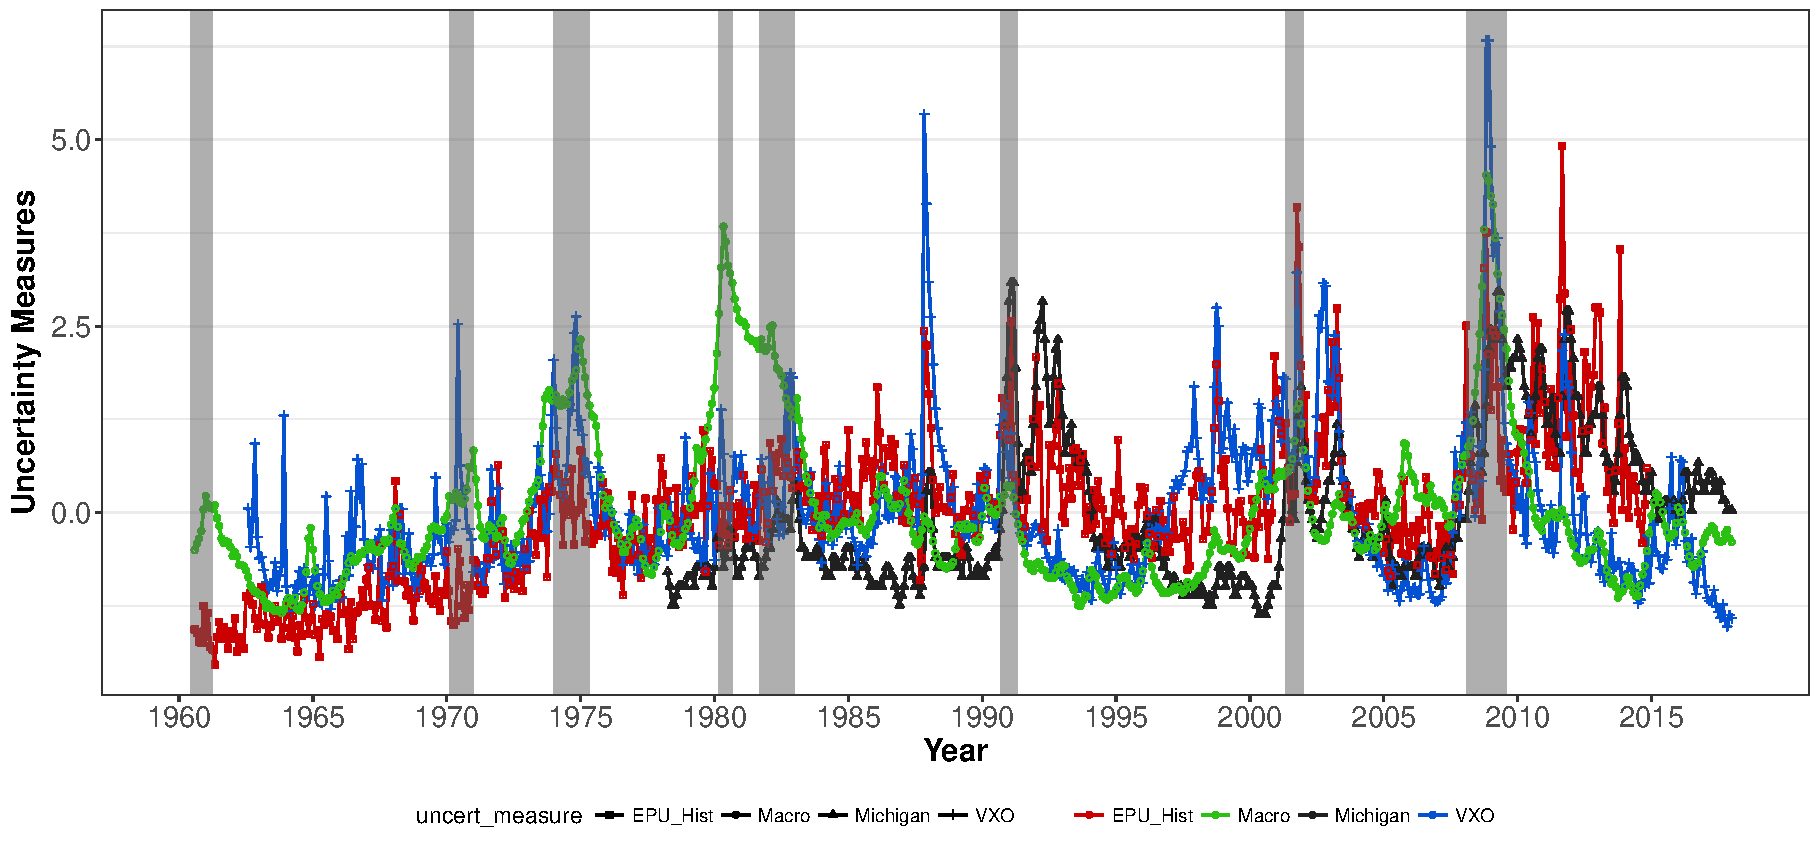
\includegraphics[trim=1cm -1.5cm 0.8cm -0cm, width=0.95\textwidth]{comparison_plot_combined.pdf}}
      \caption[Comparison of uncertainty measures.]{Comparison of uncertainty measures (facetted).
      \textit{Note:} Shaded areas denote NBER recession dates. Data frequencies are monthly. The macro uncertainty series starts in July 1960, the EPU in January 1960 and the VXO in July 1962.}   \label{fig:comparison_plot_combined}
\end{figure}



\begin{figure}[!h]
   \centering
   \setlength\fboxsep{0pt}
   \setlength\fboxrule{0pt}
     \fbox{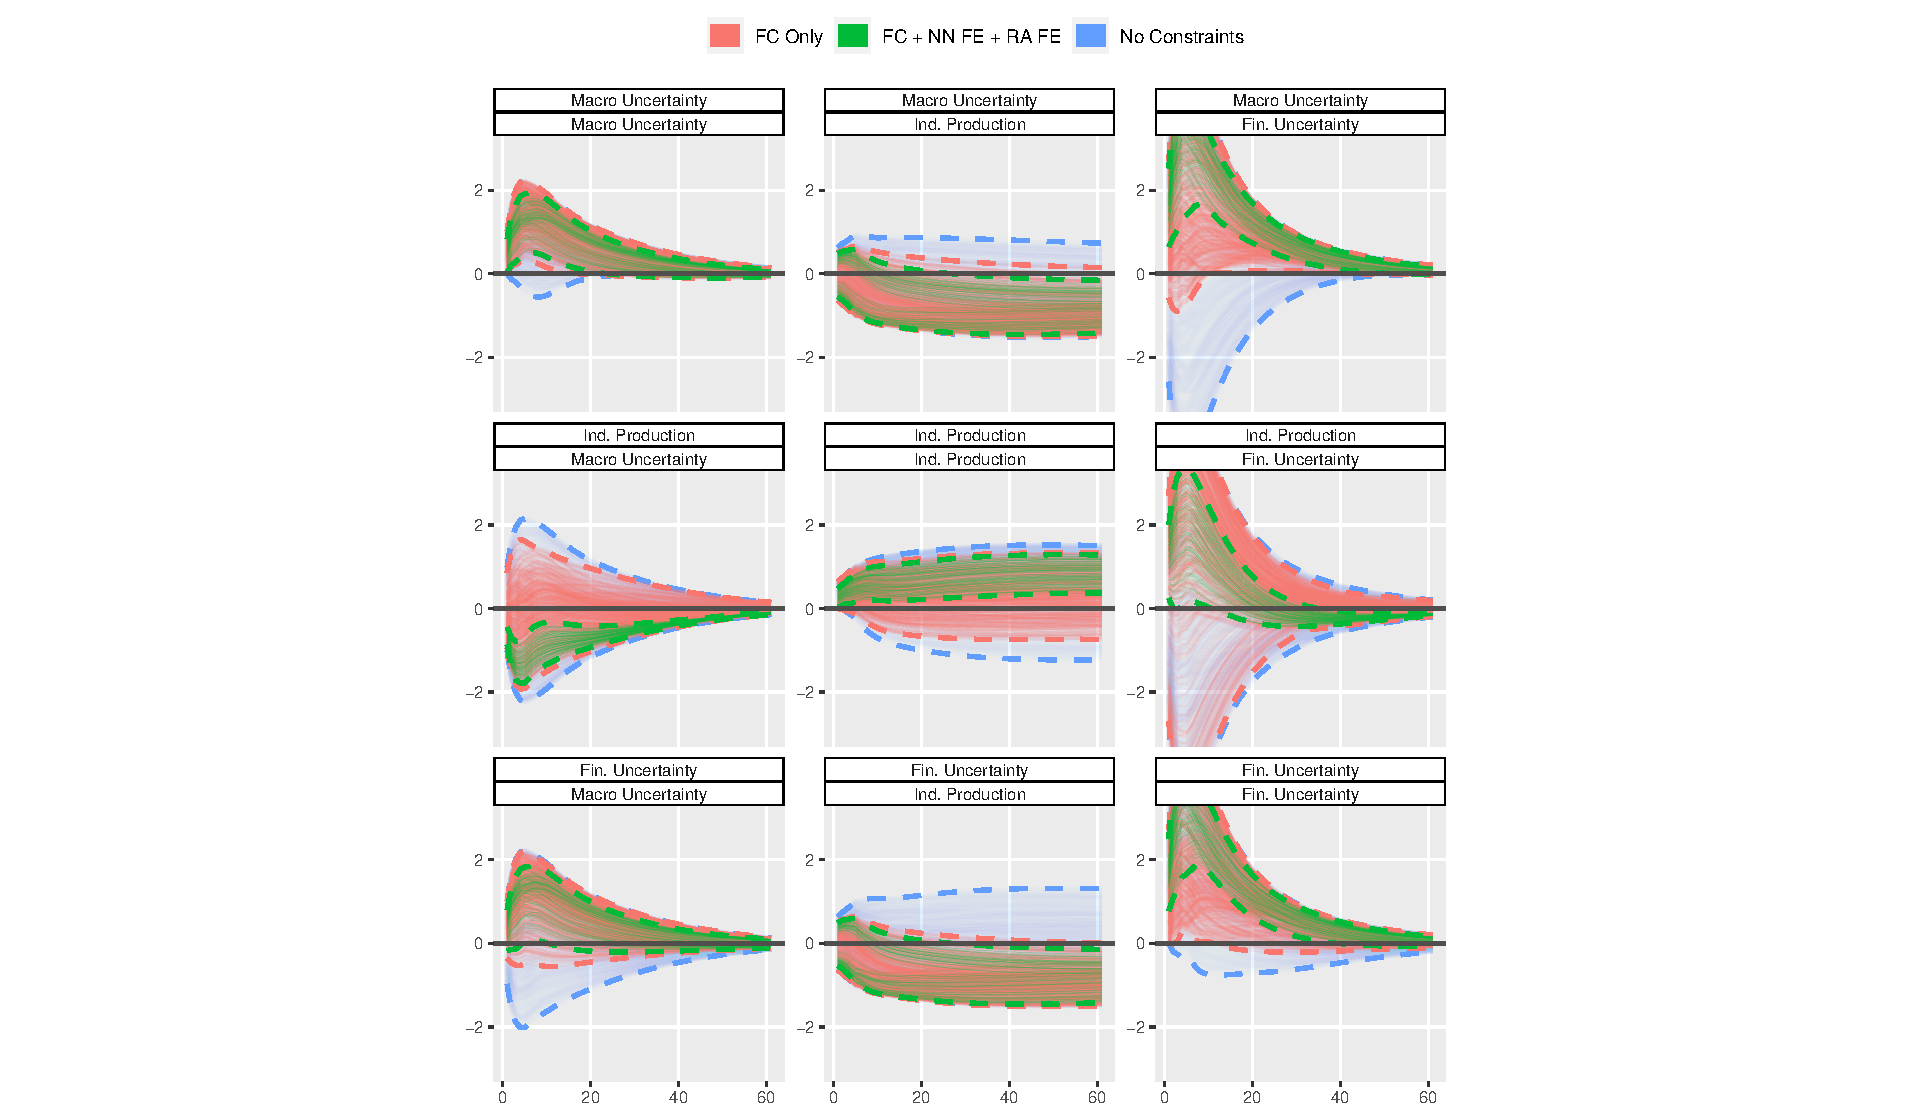
\includegraphics[trim=8cm -1.0cm -6cm -1cm, width=1.9\textwidth, clip]{impulse_responses_all_SVAR_unconstr_constr.pdf}}
      \caption[Impulse Respones from SVAR ($U_{Macro}, IPM, U_{Fin}$).]{Impulse Respones from SVAR ($U_{Macro}, IPM, U_{Fin}$).\\
      \textit{Note:} The set of solutions under 'No Constraints' are derived from switching off both of the constraints as introduced by \citet{ludvigsonetal:18}. 'Correlation Constraints Only' and 'Event Constraints Only' correspondingly show the set of solutions when only one of the two constraints are turned on. 'All Constraints' displays the \textit{identified set} and equals the solutions as shown in Figure~\ref{fig:impulse.responses_all.SVAR} which satisfy the correlation and event constraints. The selected bounds are $\overline{\lambda}_1 = -0.05$, $\overline{\lambda}_2 = 2$, $\overline{\lambda}_3 = 0.18$, $\overline{k}_1 = 4$, $\overline{k}_2 = 4$, $\overline{k}_3 = 2$. With respect to the labeling, in each panel the bottom label stands for the response of the respective variable to the shock in the top label (the impulse).}   \label{fig:impulse.responses_all.SVAR_UNCONSTR}
\end{figure}


\section{Additional (S)VAR Results}




\chapter{Appendix}
\label{DataAndCode}
\section{Data: Sources and Description}
\label{sec:dataAppendix}
Table~\ref{tab:data_sources} lists all data and their sources that appear in the main text.
\vspace*{350px}

\begin{table}[!h]
\caption[Data Sources.]{Data Sources.\\
\textit{Note:} Federal Reserve Economic Data (FRED); Chicago Board Options Exchange (CBOE); Michigan Survey of Consumers (MSoC); }
\renewcommand{\arraystretch}{1.5}
\resizebox{\textwidth}{!}{%
\centering % used for centering table
% note: the letter 'p' helps to vertically align all rows (even if one row has more text than others!)
\begin{tabular}{L{2.7cm}p{5.4cm}p{2.5cm}p{3.4cm}L{2.5cm}} % centered columns (4 columns)
\toprule
         Variable & Name &  Source & Code & Period \\ 
         \midrule
        $\text{IP}_t$ & Industrial Production Index (Monthly, Seasonally Adjusted) & FRED & INDPRO & 1962M07- \\
        $\text{EMPM}_t$ & All Employees: Manufacturing (Monthly, Seasonally Adjusted) & FRED & MANEMP & 1962M07- \\
                $\text{HOURS}_t$ & Average Weekly Hours of Production and Nonsupervisory Employees: Manufacturing (Monthly, Seasonally Adjusted) & FRED & AWHMAN & 1962M07- \\
         $\text{CPI}_t$ & Consumer Price Index for All Urban Consumers: All Items (Monthly, Seasonally Adjusted) & FRED & CPIAUSCSL & 1962M07- \\
 	$\text{NO capital}_t$ & Value of Manufacturers' New Orders for Capital Goods: Nondefense Capital Goods Industries (Monthly, Seasonally Adjusted) & IHS & M_178554409  & 1962M07- \\
 	$\text{NO cons}_t$ & Value of Manufacturers' New Orders for Capital Goods: Nondefense Capital Goods Industries (Monthly, Seasonally Adjusted) & IHS & M_14385863 & 1962M07- \\
         $\text{WAGE}_t$ & Average Hourly Earnings of Production and Nonsupervisory Employees: Manufacturing (Monthly, Seasonally Adjusted) & FRED & AHEMAN & 1962M07- \\
           $\text{M2}_t$ & M" Money Stock (Monthly, Seasonally Adjusted) & FRED & M2SL & 1962M07- \\
         $\text{FFR}_t$ & Effective Federal Funds Rate & FRED & FEDFUNDS & 1962M07- \\
         $\text{S\&P500}_t$ & S\&P's Common Stock Price Index: Composite (Monthly) & YAHOO Finance & S\&P 500 (^GSPC) & 1962M07- \\
         $\text{VXO}_t$ & Cboe S\&P 100 Volatility Index - VXO & CBOE & VXO & 1986M01- \\
         $\text{Michigan}_t$ & Consumer Uncertainty (Michigan Survey of Consumers) & MSoC & veh_fb_unc & 1978M03- \\
 	$\text{Macro1/3/12}_t$ & Macro Uncertainty Index & \citet{juradoetal:15}\footnote{Downloaded from \url{https://www.sydneyludvigson.com/data-and-appendixes}.} &  & 1962M07- \\
	$\text{EPU}_t$ & Economic Policy Uncertainty Index & \citet{bakeretal:15}\footnote{Downloaded from \url{http://www.policyuncertainty.com/}.} & News Based Policy Uncert Index & 1962M07- \\
	$\text{EPU Historical}_t$ & Economic Policy Uncertainty Index & \citet{bakeretal:15}\footnote{Downloaded from \url{http://www.policyuncertainty.com/}.} & News-Based Historical Economic Policy Uncertainty & 1962M07- \\
        \bottomrule
\end{tabular}
}
\label{tab:data_sources} % is used to refer this table in the text
\end{table}


\section[VAR-Equations and Identification Schemes]{VAR-Equations and Identification Schemes\footnote{Our notation 'VAR($p$) - $v$' denotes the number of lags $p$ and the number of variables included $v$.}}
\label{sec:VAREquations}
\subsubsection{Monthly VAR(12)-8 following \citet{bloom:09}}
The estimations include 12 lags and use monthly data from 06/1962-06/2008 (which excludes most of the Credit Crunch) and include (in that order; see also top-panel of \ref{eq:VAR8}): log(S\&P500 stock market index), an uncertainty measure (either the raw stock market volatility series that Bloom constructs through sticking actual realized stock market volatility and the CBOE's VXO-data, available as of 1986, together or various indicator variables like the 'Bloom-shock' or indicators capturing months with maximum volatility, or months capturing the first time that volatility exceeded a certain threshold; for further modifications see \citealp{bloom:09}), Federal Funds Rate, log(average hourly earnings), log(consumer price index), hours worked, log(employment), log(industrial production). Contrary to the description in \citet{bloom:09}, the STATA-code of Bloom shows that all variables except the stock market volatility series as a proxy for uncertainty are HP-detrended. Bloom's results are robust to various alternative approaches including variables ordering, variable inclusion, shock definitions, shock timing, and detrending.\\

The VARs are estimated via a recursive scheme (i.e, cholesky decomposition) based on the assumption that shocks instantaneously influence the stock market (levels and volatility), then move on to prices (wages, the consumer price index (CPI), and interest rates), and finally eventually affect quantities (hours, employment and output). In particular, \citet{bloom:09}'s rationale for including the stock-market levels as the first variable in the ordering is to ensure that the impact of stock-market levels is already controlled for when looking at the impact of volatility shocks (see \citealp[p. 630]{bloom:09}). Further, \citet{bloom:09} detrends all variables that enter the VARs using the HP-filter (\citealp{hodrickandprescott:97}) apart from the uncertainty measure(s).\footnote{In vector~\ref{eq:VAR8} all variables that enter the VAR detrended are marked with a $c$-prefix to indicate that the variable denotes the remaining cycle-component after removal of the trend.}

\citet{juradoetal:15} replicate \citet{bloom:09}'s VARs in their contribution, renounce to detrend the variables however, arguing that the HP filter uses information over the entire sample which makes it difficult to interpret the timing of an observation (hence, their specification is equal to the lower part of \ref{eq:VAR8}) and report results using \citet{bloom:09}'s original detrended variables in their Appendix.

\begin{equation} \label{eq:VAR8}
\begin{split}
\vect{y_t} &  = 
 \begin{bmatrix} 
 		y_{1t} \\
		y_{2t} \\
		y_{3t} \\
		y_{4t} \\
		y_{5t} \\
		y_{6t} \\
		y_{7t} \\
		y_{8t} 
	      \end{bmatrix} = 
 \begin{bmatrix} \text{c-log(S\&P500 Index)} \\ 
				      \textit{uncertainty measure}\\ 
				      \text{c-federal funds rate}\\
				      \text{c-log(wages)}\\
				      \text{c-log(CPI)}\\
				      \text{c-hours}\\
				      \text{c-log(employment)}\\
				      \text{c-log(industrial production)}
	      \end{bmatrix}\\\\
\vect{y_t} & = 
 \begin{bmatrix} 
 		y_{1t} \\
		y_{2t} \\
		y_{3t} \\
		y_{4t} \\
		y_{5t} \\
		y_{6t} \\
		y_{7t} \\
		y_{8t} 
	      \end{bmatrix} = 	      
	      \begin{bmatrix} \text{log(S\&P500 Index)} \\ 
				      \textit{uncertainty measure}\\ 
				      \text{federal funds rate}\\
				      \text{log(wages)}\\
				      \text{log(CPI)}\\
				      \text{hours}\\
				      \text{log(employment)}\\
				      \text{log(industrial production)}
	      \end{bmatrix}
\end{split}
\end{equation}



\subsubsection{Monthly VAR(12)-11 following \citet{juradoetal:15}}
\begin{equation} \label{eq:VAR19}
\begin{split}
\vect{y_t} & = 
 \begin{bmatrix} 
 		y_{1t} \\
		y_{2t} \\
		y_{3t} \\
		y_{4t} \\
		y_{5t} \\
		y_{6t} \\
		y_{7t} \\
		y_{8t} \\
		y_{9t} \\
		y_{10t} \\
		y_{11t}
	      \end{bmatrix} = 	      
	      \begin{bmatrix} \text{log($\text{IP}_t$)} \\ 
				      \text{log($\text{EMPM}_t$)}\\ 
				      \text{log(real consumption)}\\
				      \text{log($\text{PCE deflator}_t$)}\\
				      \text{log($\text{NO}_t$ $=$ $\text{NO capital}_t$ $+$ $\text{NO cons}_t$)}\\
				      \text{log($\text{WAGE}_t$)}\\
				      \text{log($\text{HOURS}_t$)}\\
				      \text{$\text{FFR}_t$} \\
				      \text{log($\text{S\&P500}_t$)} \\
				      \text{growth rate of $\text{M2}_t$} \\
				      \text{\textit{uncertainty (various measures)}}
	      \end{bmatrix}
\end{split}
\end{equation}

\subsubsection{Quarterly VAR(4)-8 following \citet{gilchristetal:14}}
The VARs are estimated via a standard recursive ordering technique over the 1963:Q3-2012:Q3 period using four lags of each endogenous variable. Both identification schemes employ a standard recursive ordering technique.\\

\textbf{Identification Scheme I:}
Innovations in uncertainty are assumed to have an immediate impact on credit spreads and short-term interest rates, but affect economic activity and prices with a lag. Both, shocks to uncertainty and credit spreads (financial shock) are analyzed.
\begin{equation} \label{eq:VAR20}
\begin{split}
\vect{y_t} & = 
 \begin{bmatrix} 
 		y_{1t} \\
		y_{2t} \\
		y_{3t} \\
		y_{4t} \\
		y_{5t} \\
		y_{6t} \\
		y_{7t} \\
		y_{8t} 
	      \end{bmatrix} = 	      
	      \begin{bmatrix} \text{log(real business fixed investment)} \\ 
				      \text{log(real personal consumption expenditure on durable goods)}\\ 
				      \text{log(real PCE on nondurable goods and services)}\\
				      \text{log(real GDP)}\\ 
				      \text{log(GDP deflator)}\\
				      \text{\textit{proxy for uncertainty at aggregate level}}\\
				      \text{10-year BBB-Treasury credit spread}\\
				      \text{nominal effective federal funds rate}
	      \end{bmatrix}
\end{split}
\end{equation}	

\textbf{Identification Scheme II:}      
Identification Scheme II reverses the causal ordering of the uncertainty proxy and of the variable for the 10-year BBB-Treasury credit spread to analyze the implications of uncertainty shocks conditional on the information contained in the current level of credit spreads.
\begin{equation} \label{eq:VAR21}
\begin{split}
\vect{y_t} & = 
 \begin{bmatrix} 
 		y_{1t} \\
		y_{2t} \\
		y_{3t} \\
		y_{4t} \\
		y_{5t} \\
		y_{6t} \\
		y_{7t} \\
		y_{8t} 
	      \end{bmatrix} = 	      
	      \begin{bmatrix} \text{log(real business fixed investment)} \\ 
				      \text{log(real personal consumption expenditure on durable goods)}\\ 
				      \text{log(real PCE on nondurable goods and services)}\\
				      \text{log(real GDP)}\\ 
				      \text{log(GDP deflator)}\\
				      \text{10-year BBB-Treasury credit spread}\\
				      \text{\textit{proxy for uncertainty at aggregate level}} \\
				      \text{nominal effective federal funds rate}
	      \end{bmatrix}
\end{split}
\end{equation}

\subsubsection{Quarterly VAR(4)-8 following \citet{basuandbundick:17}}
\citet{basuandbundick:17} include the VXO as a measure of uncertainty, gross domestic product (GDP), consumption, investment, hours worked, the GDP deflator, the M2 money stock, and a measure of the monetary policy stance (in that order) over the 1986-2014 sample period including four lags. All variable apart from the monetary policy measure enter the VAR in log levels. Identifying the uncertainty-shock using a Cholesky decomposition with the VXO ordered first, the authors assume that uncertainty shocks can affect output and its components immediately but that other variables' shocks, however, do not influence the VXO on impact. 
\begin{equation} \label{eq:VAR22}
\begin{split}
\vect{y_t} & = 
 \begin{bmatrix} 
 		y_{1t} \\
		y_{2t} \\
		y_{3t} \\
		y_{4t} \\
		y_{5t} \\
		y_{6t} \\
		y_{7t} \\
		y_{8t} 
	      \end{bmatrix} = 	      
	      \begin{bmatrix} \text{\textit{log(uncertainty (VXO))}} \\ 
				      \text{log(GDP)}\\ 
				      \text{log(consumption)}\\
				      \text{log(investment)}\\ 
				      \text{log(jours worked}\\
				      \text{log(GDP deflator)}\\
				      \text{log(M2 money stock)} \\
				      \text{measure of monetary policy stance}
	      \end{bmatrix}
\end{split}
\end{equation}




\subsubsection{Monthly VAR(?)-4 following \citet{leducandliu:16}}
The four-variable BVAR on US data consists of a measure of uncertainty, the unemployment rate, the CPI year-on-year inflation rate and a short-term interest rate (as represented by the three-month Treasury bills rate). As a measure of uncertainty, \citet{leducandliu:16} use both, the VIX/VXO and data from the Michigan survey (consumers' perceived uncertainty constructed from the Thomson Reuters/University of Michigan Surveys of Consumers). Their rationale for using a consumer uncertainty measure is that, by construction of the survey, interviewees do not have (complete) information of the current month's macroeconomic data. Hence, it is assumed that survey participants will condition their answers on all previous realizations of macroeconomic indicators except time $t$. With their identification strategy \citet[p. 23]{leducandliu:16} assume that their ``[...] measured uncertainty contains \textit{some}\footnote{Author's italics.} exogenous component and does not reflect endogenous responses of other macroeconomic variables. In the model including the VIX/VXO, the sample ranges from 01:1986-10:2013, in the models with the consumer uncertainty measure from 01:1978-10:2013. Further, placing the uncertainty measure first in their Choleski ordering hence implies that on impact of a shock only unemployment, inflation and the nominal interest rate are allowed to respond.
\begin{equation} \label{eq:VAR22}
\begin{split}
\vect{y_t} & = 
 \begin{bmatrix} 
 		y_{1t} \\
		y_{2t} \\
		y_{3t} \\
		y_{4t}
	      \end{bmatrix} = 	      
	      \begin{bmatrix} \text{\textit{measure of uncertainty}} \\ 
				      \text{unemployment rate}\\ 
				      \text{inflation rate (CPI)}\\
				      \text{three-month Treasury bills rate}
	      \end{bmatrix}
\end{split}
\end{equation}

%\newgeometry{left=25mm, right=25mm, top=30mm, bottom=30mm}
%the below code is to adjust the header ruler after the
%newgeometry!
%\fancyhfoffset[E,O]{0pt}
%\section{Code}
%\label{sec:rcode}

%\subsection{SVAR-Framework of \citet{ludvigsonetal:18}}
%\label{sec:codeSVAR_LMN}
%\begin{Verbatim}[fontsize=\small]
%halloe
%\end{Verbatim} 

%\begin{verbatim}
%halloe
%\end{verbatim} 

%\begingroup
%\fontsize{9pt}{12pt}\selectfont
%\begin{verbatim}  
%##The Code will go here.
%
%
%
%
%\end{verbatim}  
%\endgroup


\restoregeometry

%%%%%%%%%%%%%%%%%%%%%%%%%BIBLIOGRAPHY%%%%%%%%%%%%%%%%%%%%%%%%%%%%
%%%%%%%%%%%%%%%%%%%%%%%%%BIBLIOGRAPHY%%%%%%%%%%%%%%%%%%%%%%%%%%%%
%%%%%%%%%%%%%%%%%%%%%%%%%BIBLIOGRAPHY%%%%%%%%%%%%%%%%%%%%%%%%%%%%

\nocite{*}
\clearpage
\thispagestyle{empty}
\bibliographystyle{agsm}
%bibliographystyle{agsm} bewirkt, dass KEINE Beistriche zwischen den Jahreszahlen sind. Dafür aber
%Gänsefüßchen beim Titel der Werke!
\bibliography{mybiblio}





%%%%%%%%%%%%%%%%%%%%%%EIDESSTATTLICHE ERKLÄRUNG%%%%%%%%%%%%%%%%%%%%%%
\clearpage
\thispagestyle{empty}
\null\vspace{46pt}
\paragraph{\large{Declaration of Authorship}}
\vspace{43pt}
I hereby declare that I prepared this master's thesis independently and that the thoughts taken
directly or indirectly from other sources are acknowledged as references accordingly. \\
\\
The work contained in this thesis has neither been previously submitted to any other examination authority nor published in any other form which has led to the award of a degree.\\[10mm]

    Innsbruck, \makebox[1.8in][l]{\hrulefill} \qquad \makebox[2.6in]{\hrulefill}\\
    \makebox[2.95in][l]      \hfill\makebox[2.0in][l]{(Signature: Marcel Kropp)}

\clearpage
\thispagestyle{empty}
\null\vspace{46pt}
\paragraph{\large{Eidesstattliche Erklärung}}
\vspace{43pt}
Ich erkläre hiermit an Eides Statt, dass ich dir vorliegende Masterarbeit selbständig angefertig habe. Die aus fremden Quellen direkt oder indirekt übernommenen Gedanken sind als solche kenntlich gemacht. \\
\\
Die Arbeit wurde bisher weder in gleicher noch in ähnlicher Form einer anderen Prüfungsbehörde vorgelegt und auch noch nicht veröffentlicht.\\[10mm]

    Innsbruck, \makebox[1.8in][l]{\hrulefill} \qquad \makebox[2.6in]{\hrulefill}\\
    \makebox[2.95in][l]      \hfill\makebox[2.0in][l]{(Unterschrift: Marcel Kropp)}


%%%%%%%%%%%%%%%%%%%%%%EIDESSTATTLICHE ERKLÄRUNG%%%%%%%%%%%%%%%%%%%%%%

\end{document}
%%%%%%%%%%%%%%%%%%%%%%END OF THE DOCUMENT%%%%%%%%%%%%%%%%%%%%%%%%%%
%%%%%%%%%%%%%%%%%%%%%%END OF THE DOCUMENT%%%%%%%%%%%%%%%%%%%%%%%%%%
%%%%%%%%%%%%%%%%%%%%%%END OF THE DOCUMENT%%%%%%%%%%%%%%%%%%%%%%%%%%